\documentclass[a4paper]{article}
%\pagestyle{page}
\usepackage{graphicx}
\usepackage{html}
\usepackage{ifpdf}
\usepackage{fancyhdr}
\newcommand{\oofem}{\htmladdnormallink{OOFEM}{http://www.oofem.org}\ }
\newcommand{\bp}{\htmladdnormallink{Bo\v{r}ek Patz\'{a}k}{http://mech.fsv.cvut.cz/~bp/bp.html}}

\oddsidemargin -10mm
\evensidemargin -10mm
\textwidth 180mm
\parindent 0mm

\renewcommand{\topfraction}{0.99}	% 99% of page top can be a float
\renewcommand{\bottomfraction}{0.99}	% 99% of page bottom can be a float
\renewcommand{\textfraction}{0.01}	% only 1% of page must to be the text
\renewcommand{\floatpagefraction}{0.99} % 99% of whole page can be a float
\setcounter{totalnumber}{5} %maximum floating objects on one page

\newcommand{\class}[1]{{\bf #1}}
\newcommand{\service}[1]{{\em #1}}
\newcommand{\attribute}[1]{#1}
\newcommand{\file}[1]{``#1''}
\newcommand{\refman}{\oofem library reference manual}

\newcommand{\mbf}[1]{\mbox{\boldmath$#1$}}
\font\mbff=cmbsy10\def\mbfx#1{\hbox{\mbff#1}}%\let\mbf\Mbff
\newcommand{\del}[2]{\mbox{$\displaystyle\frac{#1}{#2}$}}

\headheight 15pt
\pagestyle{fancy}{
\fancyhf{}
\fancyhead[L]{\slshape \leftmark}
\fancyhead[R]{\thepage}
}

\begin{document}
%begin{latexonly}
\title{
\ifpdf
\oofemlnk{\centerline{
\includegraphics[width=0.7\textwidth]{oofem-logo-contour.pdf}}}
\else
\oofemlnk{\centerline{
\includegraphics[width=0.7\textwidth]{oofem-logo-contour.eps}}}
\fi
Programmers's manual}
\author{\bp \\ \\
Czech Technical University\\
Faculty of Civil Engineering\\
Department of Structural Mechanics\\
Th\'akurova 7, 166 29 Prague, Czech Republic
}
\maketitle
%end{latexonly}
\begin{htmlonly}
\begin{center}
\oofemlnk{\centerline{
\includegraphics[width=0.7\textwidth]{oofem-logo-contour.eps}}}
{\Large Programmers's manual}\\ \\
{\bp \\ 
Czech Technical University\\
Faculty of Civil Engineering\\
Department of Structural Mechanics\\
Th\'akurova 7, 166 29 Prague, Czech Republic
}
\end{htmlonly}

\latex{\clearpage}
\html{\newline\newline\htmlrule\newline}
\begin{center}
{\large \bf LEGAL NOTICE}
\end{center}\vspace*{1cm}
\centerline{Copyright (C) 2000 Bo\v{r}ek Patz\'{a}k}\vspace{1cm}
\begin{center}
{\bf This notice must be preserved on all partial or complete copies
of this manual. All modifications to this manual, translations or
derivative work based on this manual must be first approved in writing
by the author. If part of this manual is distributed, a notice how to
obtain the full version must be included.}\\

\begin{verbatim}
    The OOFEM is free software; you can redistribute it and/or modify
    it under the terms of the GNU General Public License as published by
    the Free Software Foundation; either version 2 of the License, or
    (at your option) any later version.

    This program is distributed in the hope that it will be useful,
    but WITHOUT ANY WARRANTY; without even the implied warranty of
    MERCHANTABILITY or FITNESS FOR A PARTICULAR PURPOSE.  See the
    GNU General Public License for more details.

    You should have received a copy of the GNU General Public License
    along with this program; if not, write to the Free Software
    Foundation, Inc., 675 Mass Ave, Cambridge, MA 02139, USA.                                                               
\end{verbatim}

{\bf The author is not liable for any damages, direct or indirect,\\
resulting from the use of the information provided in this work.}
\end{center}
\clearpage
\tableofcontents
\clearpage

\section{Introduction}

The aim of OOFEM project is to develop efficient and robust tool for
FEM computations as well as to provide modular and extensible
environment for future development.

The aim of this document is to provide the introduction to the OOFEM
principles and internal structure. However, it is not intended to
contain the detailed description of the whole package. Interested readers
should follow the \refman\footnote{http://ksm.fsv.cvut.cz/oofem/oofem.html} for more
detailed reference. This hypertext reference
manual is generated automatically from the source code and it
represents always up to date source of information. It contains a class
hierarchy browser, an alphabetical list of all components and a
detailed hypertext description of all library components, including
all classes and their attributes and services.


The OOFEM comes divided into two basic parts - a library and
a distribution. The library (called OOFEMlib) is the core part of the OOFEM, containing
the basic collection of classes. These classes are problem independent
and they provide the common definitions and support to all FEM
problems. The distribution part contains the rest - modules representing the problem dependent
parts. 

The OOFEM package is written in C++ (see, for example \cite{c++}, for reference). This 
document contains many examples and listings of a parts of the source
code. Therefore, the ideal reader should be familiar with C++ programming
language. However, any reader with an object-oriented background should
follow this document, since the examples are written in a form, which is 
easy to read and understand.

\section{General Structure}
%Let us move to the next part of presentation, to the description of
%structure of  OO FEM program.

General structure is shown in Fig.~\ref{genstructfig}.
The key class is \class{EngineeringModel} representing the problem
under consideration. It can contain one or more domains (abstractions
for computational mesh) represented by the \class{Domain} class.
Generally
speaking, it contains the domain description, or if the program runs in
parallel, then it contains the description of the domain associated
with a particular processor or thread of execution. \class{Domain} 
contains and manages lists of degree of freedom managers, elements, boundary
conditions, cross sections, and material models - these describe the geometry
of the problem, its constitutive properties, and applied boundary
conditions. Services for accessing each of these objects are
provided. 
\class{Domain} class \& object provides services for reading input
files and instantiating corresponding components accordingly. 


\begin{figure}[tb]
\begin{htmlonly}
  %\htmlimage{thumbnail=0.9,flip=r270}
  \htmlimage{thumbnail=0.9,flip=r270}
  \centerline{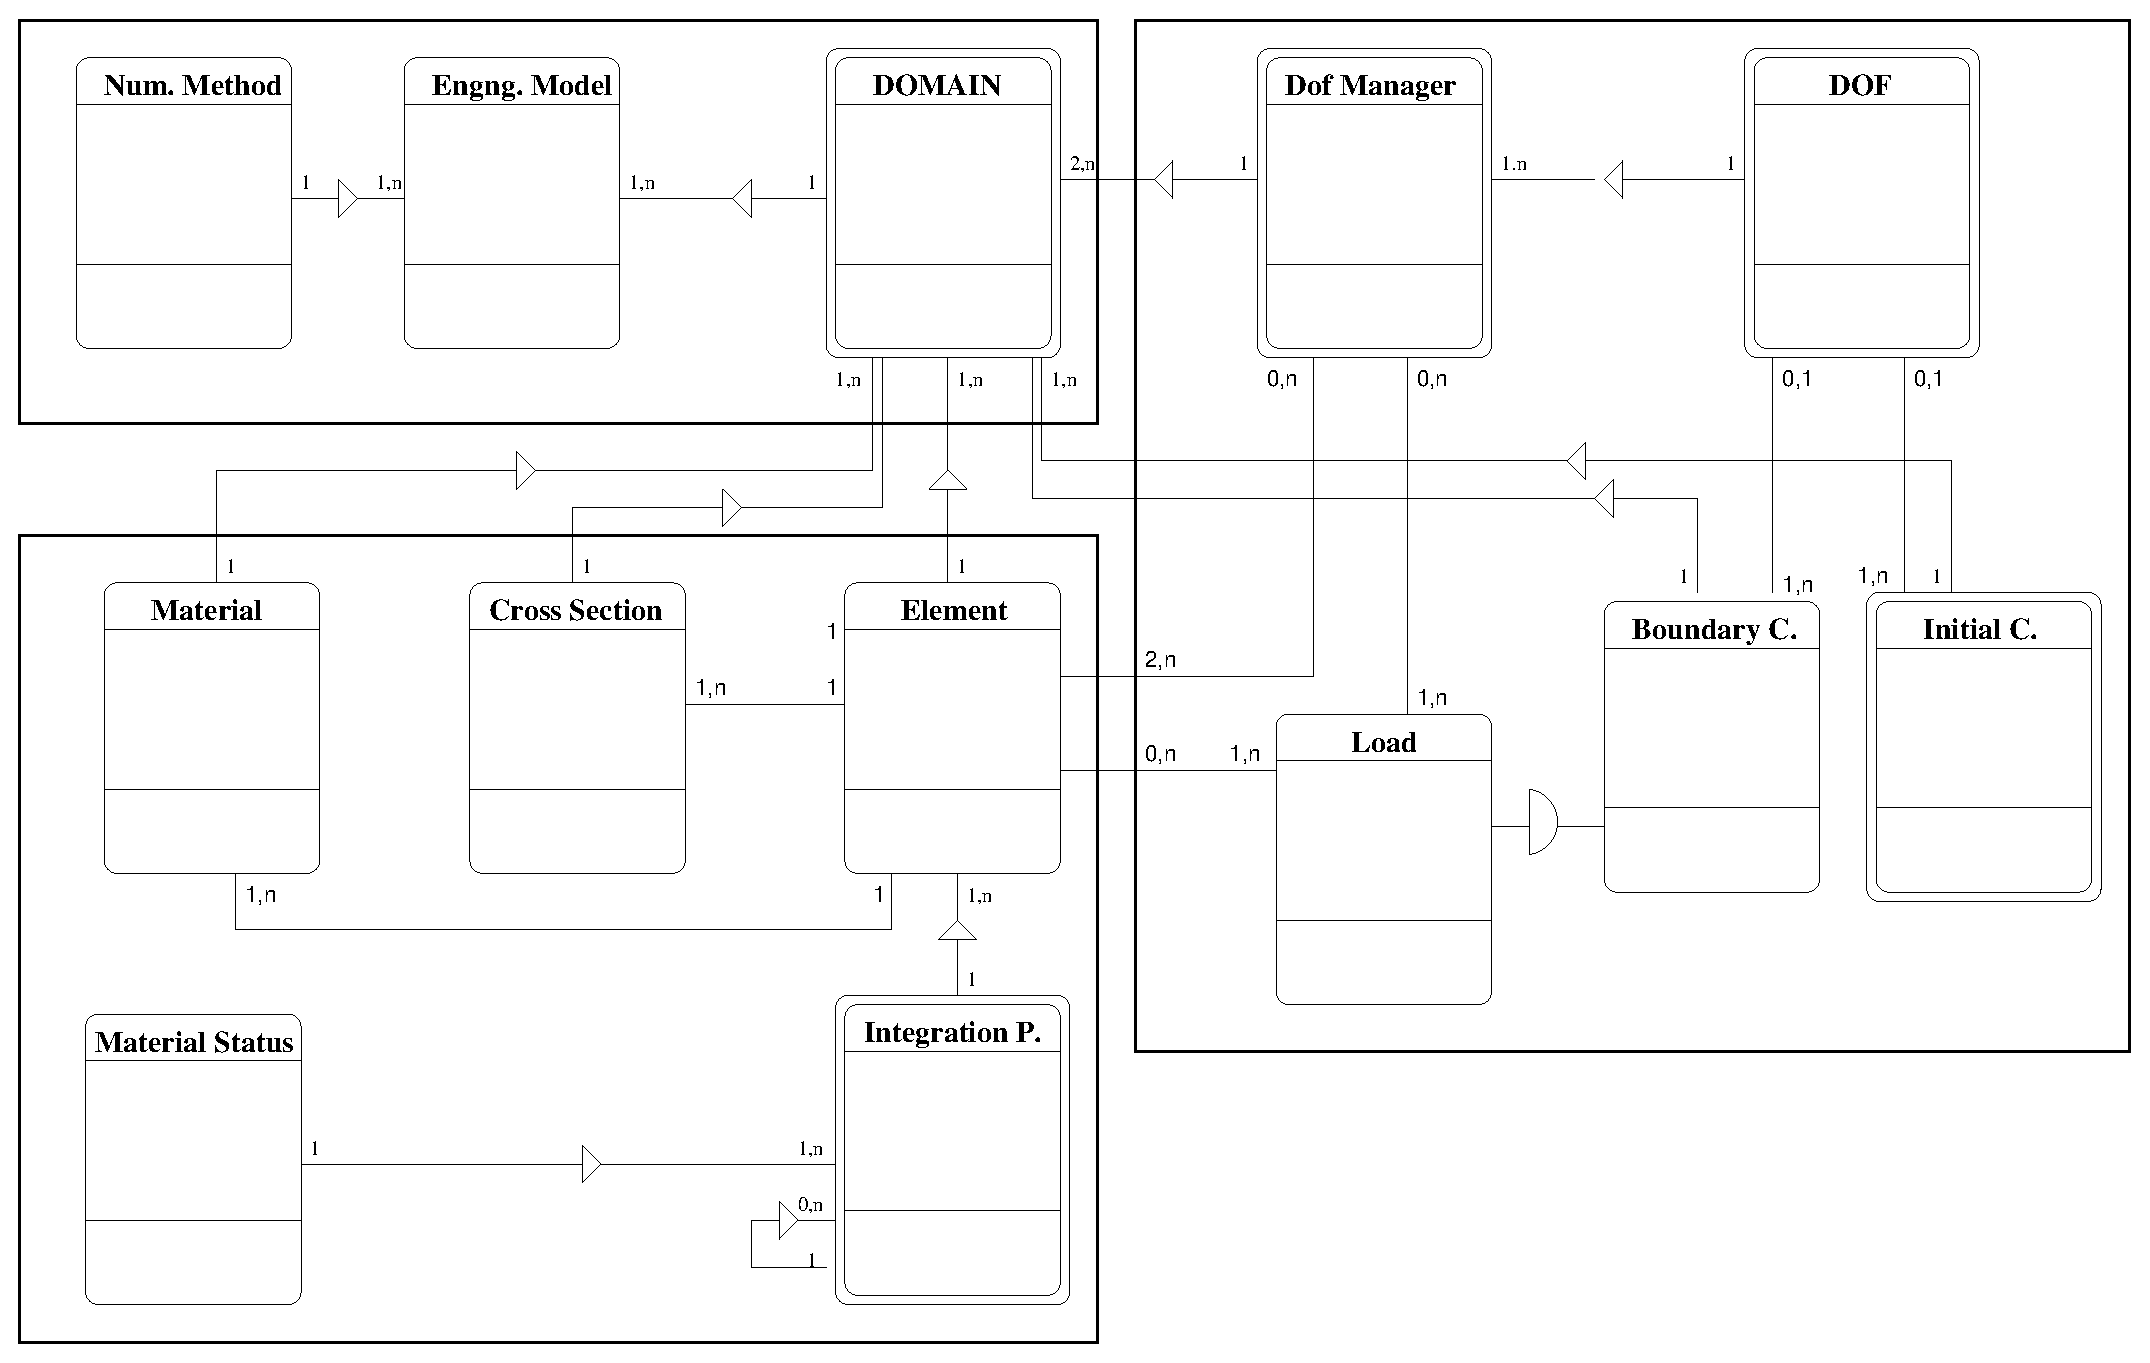
\includegraphics[width=0.7\textwidth]{general.eps}}
\end{htmlonly}
%begin{latexonly}
\ifpdf
\centerline{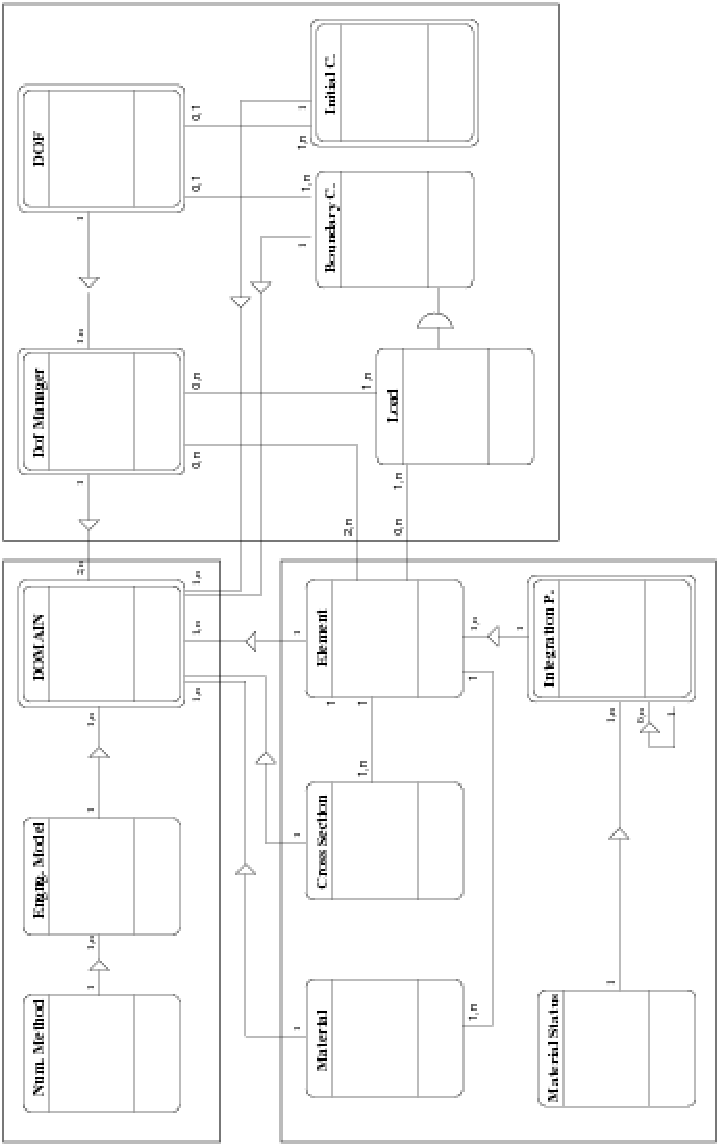
\includegraphics[angle=270,width=0.7\textwidth]{general.pdf}}
\else
\centerline{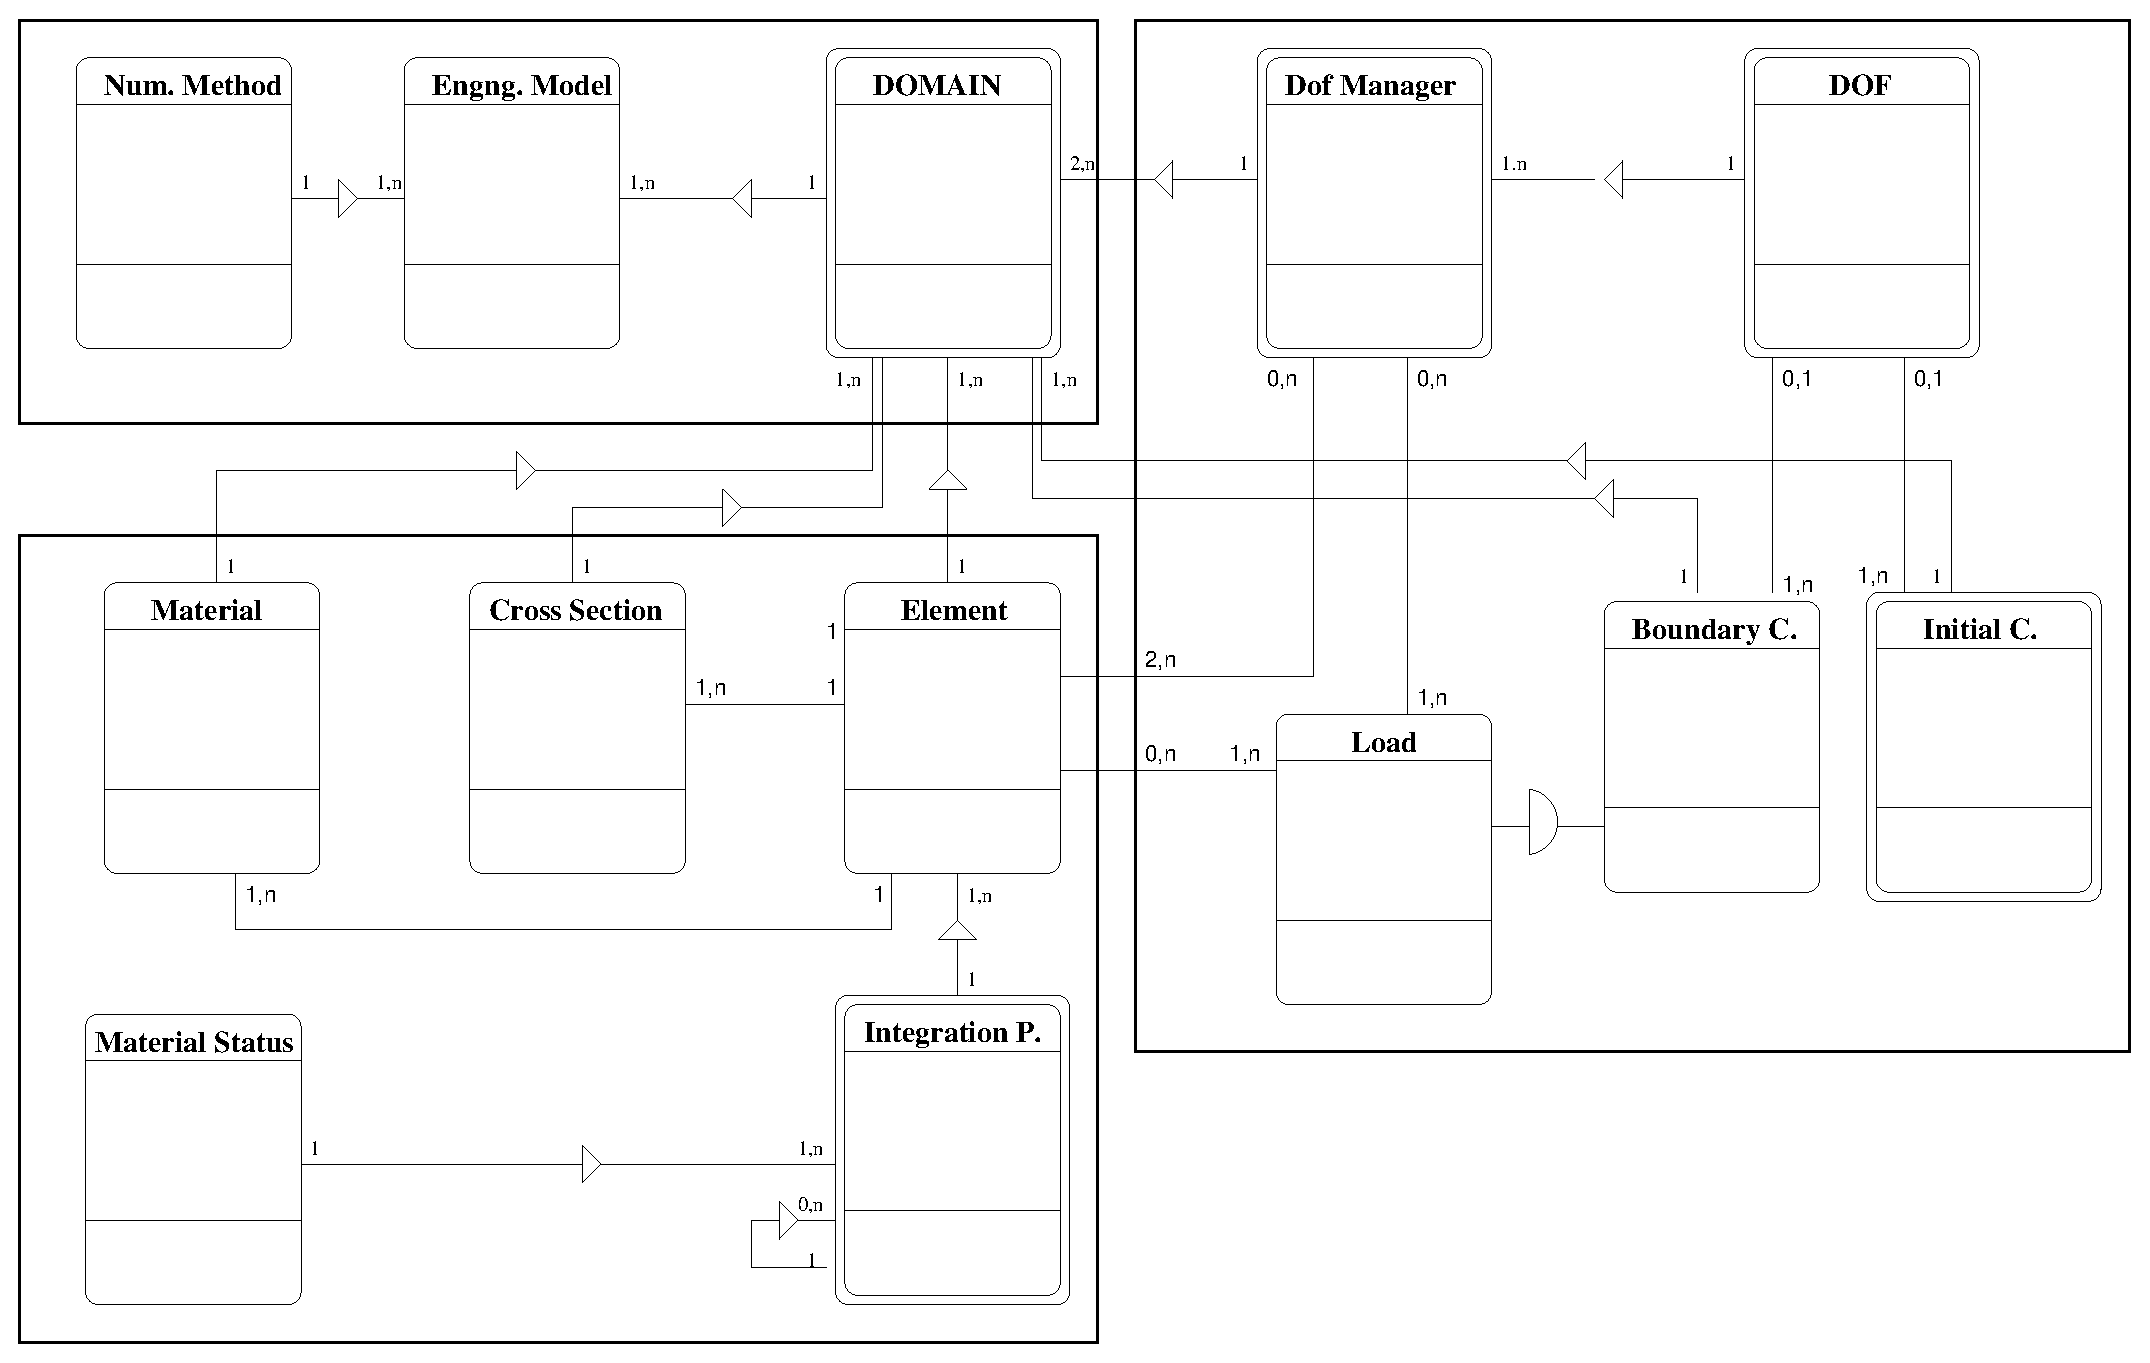
\includegraphics[width=0.7\textwidth]{general.eps}}
\fi
%end{latexonly}
\caption{General Structure.}
\label{genstructfig}
\end{figure}

Engng model and Numerical method interfaces, shown schematically in
top-left frame, will be explained in
Section~\ref{engngNummetsection}. The classes \& objects in the left-bottom frame represent the element,
material model, and cross section abstractions. Because of their
principal importance, a special 
section~\ref{materialEleemntFrame} will be devoted to a detailed
explanation of this frame. 

\class{DOF} is an abstraction for a single degree of freedom (DOF). It maintains
its physical meaning and associated equation number. \class{DOF} is
the attribute of \class{DofManager}. The \class{DofManager} manages the collection
of DOFs. A typical
derived class is class \class{Node}, representing a node in a finite element mesh.
\class{Boundary condition} and \class{Initial condition} are abstractions of boundary and
initial conditions. They are attributes of \class{Domain} and are associated
with one or more \class{DOF}s. The abstract class \class{Load}, derived from base \class{Boundary
condition} class, is an abstraction for load. It is an attribute of \class{Domain}
and can be associated with several dof managers or elements, according to
the type of loading it represents. The class declares the basic services provided by
all derived classes. Derived classes declare specific load type dependent
services and implement all necessary services.



\section {Engineering model --- Numerical Method Frame}
\label{engngNummetsection}

\subsection{Problem representation - Engineering model}
\class{Engng model} is an abstraction for the problem under
consideration. It represents the type of analysis to be performed.
Base class declares and implements the basic general services for assembling
characteristic components and services for starting the solution step and
its termination. Derived classes ``know'' the form of governing
equation and the physical meaning of  particular components. 
They are responsible for forming the governing equation for each solution
step,  usually by summing contributions from particular elements and
nodes.

The solution step may represent either a time step, a load increment, or a load
case. The solution steps are grouped together into so called meta steps. 
The meta step can be thought as a sequence of
solution steps, with the same set of attributes used to drive the behavior of
engng model.
For each meta step, the engng model typically updates  
certain attribute values  according to meta step model  attributes (see
updateAttributes service) and creates the solution steps
accordingly. This allows to switch to a different time increment, 
a different solution control, etc. If no meta step is specified, the engng model
creates a default one for all required solution steps. There are two
services, where engng model attributes are set or updated. The first one,
used for those attributes which do not vary during the solution 
of the problem, are initialized  in \service{instanciateYourself} service.
The second service is \service{updateAttributes}, where the attributes 
(with meta step validity) are updated according to a values valid for the
given meta step.
If no meta step is introduced, a default one is created 
(with the attributes set to the engng model attributes). 
Then there is no difference, whether the attributes are initialized 
in instanciateYourself or in updateAttributes, but
the preferred scheme is to read all attributes in instanciateYourself 
and to left updateAttributes service empty.

The basic EngngModel tasks are following:
\begin{itemize}
\item
Assembling governing equations by summing contributions 
(typically from nodes and elements).
\item
Solving the problem described by governing equation(s) using the instance of
a suitable numerical method. This requires to establish a mapping between numerical method-parameters 
and EngngModel components of governing equation.
EngngModel must map each component of governing
equation(s) (which has physical meaning) to the corresponding numerical component.
This mapping between physical components to independent numerical components 
(understood by the numerical method) is important, because it allows
the numerical method to be used by
many EngngModels with different component meaning and allows to use 
different numerial methods by EngngModel. This is achieved by using
the compulsory numerical component names (see further).
\item
Providing access to the problem solution. Services for returning unknown
values according to their type and mode are provided. These services are used by DOFs to 
access their corresponding unknowns.
\item
Terminating the time step by updating the state of the problem domains (nodes and
elements, including integration points).
\item
Managing the problem domains, meta steps, and problem input/output
streams.
\item
Equation numbering.
\item 
Storing and restoring problem state to/from context file.
\item
Updating the DOF unknown dictionaries if EngngModel supports changes of
static system (see the Dof class 
documentation for detailed explanation). In general, if the static system changes are not supported,
then when the DOFs are asked for unknowns, they use their equation numbers to ask EngngModel
for corresponding unknowns. The unknown values are therefore stored in
the EngngModel and are requested by the DOFs.
On the other hand, when the changes of the static system are supported, the equation numbers of DOFs 
can vary during the solution. Therefore, so called DOF unknown dictionaries are introduced.
All unknowns are stored on the DOF level and the DOFs will use in such case their own dictionaries
instead of requesting the EngngModel. The EngngModel is then fully responsible for updating this
dictionaries for each DOF with all necessary unknowns (see updateDofUnknownsDictionary function).
\end{itemize}

The complete listing of \class{EngngModel} class declaration folows.  

{\small\begin{verbatim}
/* $Header: /home/cvs/bp/oofem/doc/usrman/usrman.tex,v 1.7 2003/04/23 14:19:27 bp Exp $ */


//   ************************
//   *** CLASS ENGNGMODEL ***
//   ************************
class EngngModel 
{

protected:
 /// number of receiver domains
 int ndomains;
  /// List of problem domains
 AList<Domain>*    domainList;
 /// Total number of time steps 
 int       numberOfSteps;
 /// total number of equation in cuurent time step
 int       numberOfEquations;
  /// total number or prescribed equations in current time step
 int       numberOfPrescribedEquations;
  /// number of equations per domain
 IntArray  domainNeqs;
  /// number of prescribed equations per domain
 IntArray  domainPrescribedNeqs;
  /// renumbering flag
 int renumberFlag;
  /// equation numbering completed flag
 int equationNumberingCompleted;
  /// number of meta steps
 int nMetaSteps;
  /// List of problem metasteps
 AList<MetaStep>* metaStepList;
  /// Solution step when IC (initial conditions) apply
 TimeStep* stepWhenIcApply;
 /// Currnet time step
 TimeStep* currentStep ;
 /// Previous time step
 TimeStep* previousStep;
  /// receivers id 
 int      number ;

  /// Path to input stream
 //char*                 dataInputFileName ;
 /// Path to output stream
 char*                   dataOutputFileName ;
 /// Output stream 
 FILE* outputStream;
 /// Input stream 
 //FILE* inputStream;
 /// Domain context output mode
 ContextOutputMode       contextOutputMode;
 int                     contextOutputStep;

  ///Export module manager
  ExportModuleManager* exportModuleManager; 


 /// Domain mode
 problemMode             pMode ;
 /// solution start time
 time_t startTime;
 // initial value of processor time used by program
 // clock_t startClock;

  /// master e-model; if defined receiver is in maintained (slave) mode
  EngngModel* master;
  /// context
  EngngModelContext* context;
 /**
    flag indicating that the receiver runs in parallel.
 */
 int parallelFlag;


public:
 /**
  Constructor. Creates Engng model with number i belonging to domain d.
  */
 EngngModel (int i, EngngModel* _master = NULL) ;    // constructor
  /**
   Constructor. Creates Engng model with number i and input file given by path.
  */
  EngngModel (int i, char* s, EngngModel* _master = NULL);
 /// Destructor.
 virtual ~EngngModel ()  ;      // destructor

  /**
  Service for accessing particular problem domain.
  Generates error if no such domain is defined.
  @param: n pointer to n-th domain is returned
 */
  Domain*     giveDomain (int n);
  /// Returns number of domains in problem.
 int         giveNumberOfDomains () {return ndomains;}
 /** Service for accessing ErrorEstimator corresponding to particular domain */
 virtual ErrorEstimator* giveDomainErrorEstimator (int n) {return NULL;}
 // input / output
 /// Returns input file path.
 //char*              giveInputDataFileName () ;
 /// Returns file descriptor of output file
 FILE*              giveOutputStream () ;
 /** Returns base output file name
     to which extensions, like .out .vtk .osf should be added.
     In current implementation, output file name is simply returned.
     @param path and base file name will be copied into the array pointed to by  dest
     @param not more than n bytes of src  are copied
 */
 char * giveOutputBaseFileName(char *dest, size_t n) 
        {return strncpy (dest, dataOutputFileName, n);}

 //FILE*              giveInputStream () ;
  
 /*
  Returns current time in seconds as returned by time call.
  @return current time in time_t structure.
  */
 //time_t             getTime ();
 /*
  Returns an approximation of processor time used by the program.
  The value returned is the  CPU  time  used  so  far  as  a
  clock_t;  to  get  the  number  of seconds used, divide by
  CLOCKS_PER_SEC. Calls clock ANSI C function.
  The C standard allows for arbitrary values at the start of
  the   program;  take  the  difference  between  the  value
  returned from a call to this method at the start of  the  pro-
  gram and the end to get maximum portability.
  */
 //clock_t            getClock ();
 /**
  Returns domain context output mode.
  */
 ContextOutputMode  giveContextOutputMode () {return contextOutputMode;}
 /**
  Returns domain context output step.
  */
 int                giveContextOutputStep () {return contextOutputStep;}
 /**
  Sets context output mode of receiver.
  @param contextMode domain context mode.
  */
 void               setContextOutputMode (ContextOutputMode contextMode) 
  {contextOutputMode=contextMode;}
 /**
  Sets user defined context output mode (it sets contextOutputMode to contextOutputMode), 
  setting contextOutputStep to given value.
  @param cStep new context output step
  */
 void               setUDContextOutputMode (int cStep)
  {contextOutputMode=USERDEFINED; contextOutputStep = cStep;}
 /**
  Sets domain mode to given mode.
  @param mode domain mode.
  */
 void               setProblemMode (problemMode mode) {pMode = mode;}
 /// Returns domain mode.
 problemMode         giveProblemMode ()        {return pMode;}
  /// Sets the renumber flag to TRUE
 virtual void                setRenumberFlag() {this->renumberFlag = 1;}
  /// Sets the renumber flag to FALSE
 virtual void                resetRenumberFlag() {this->renumberFlag = 0;}

 /**
  Performs analysis termination after finishing analysis.  
  */
 void               terminateAnalysis () ;
  
 // solving

 /** Starts solution process. Implementation should invoke for each
 time step solveYourselfAt function with time step as parameter. Time
 steps are created using giveNextStep function (this will set current
 time step to newly created, and updates previous step).
  */
 virtual void               solveYourself ();

 /** Solves problem for given time step. Should assemble
 characteristic matrices and vectors if necessary and solve problem
 using appropriate numerical method. After finishing solution,
 this->updateYourself function for updating solution state and then
 this->terminate function (for updating nodal and element values)
 should be called.  
 */
 virtual void               solveYourselfAt (TimeStep*) {}
 //virtual int                requiresNewLhs () {return 1;}

 /** Terminates the solution of time step. Default implementation
 calls prinOutput() service and if specified, context of whole domain
 is stored and output for given time step is printed.  
 */
 virtual void               terminate (TimeStep*);

 /** Prints the ouput of the solution step (using virtual
 this->printOutputAtservice) to the stream detemined using
 this->giveOutputStream() method and calls exportModuleManager to do
 output.  */
 virtual void              doStepOutput(TimeStep*);

 /** Saves context of given solution step, if required (determined
 using this->giveContextOutputMode() method).  
 */
 void                       saveStepContext(TimeStep*);

 /** Updates internal state after finishing time step. (for example
 total values may be updated according to previously solved
 increments).  Then element values are also updated (together with
 related integration points and material statuses).  */
 virtual void               updateYourself (TimeStep* stepN);

 /** Provides the oportunity to initialize state variables stored in
 element integration points acording to initial conditions using
 function initializeYourself() on element level.  Should be called
 when curent time step is time step when IC will aply (see
 EngngModel::giveNumberOfTimeStepWhenIcApply) somewhere from
 solveYourselfAt function). Implementation must be provided.  Default
 implementation is empty.  */
 virtual void               initializeYourself (TimeStep*) {}

  /** Initializes the newly generated discretization state acording to
  previous solution.  This process should typically include restoring
  old solution, instanciating newly generated domain(s) and by mapping
  procedure.  */
  virtual int                initializeAdaptive (int stepNumber) {return 0;}

 /** Returns total number of equations in active (current time steep)
 time step.  The UnknownType parameter allows to distinguis between
 several possible governing equations, that can be numbered
 separately.  */
 virtual int                giveNumberOfEquations (EquationID);

 /** Returns total number of prescribed equations in active (current
 time steep) time step.  The UnknownType parameter allows to
 distinguis between several possible governing equations, that can be
 numbered separately.  */
 virtual int                giveNumberOfPrescribedEquations (EquationID);

 /** Returns number of equations for given domain in active (current
 time steep) time step.  The UnknownType parameter allows to
 distinguis between several possible governing equations, that can be
 numbered separately.  */
 virtual int                giveNumberOfDomainEquations (int, EquationID);

 /** Returns number of prescribed equations for given domain in active
 (current time steep) time step.  The UnknownType parameter allows to
 distinguis between several possible governing equations, that can be
 numbered separately.  */
 virtual int                giveNumberOfPrescribedDomainEquations (int, EquationID);
 //virtual IntArray*          GiveBanWidthVector ();
      

 // management components
 /** Provides backward mapping between numerical component and
 characteristic component on EngngModel level.  */
 virtual CharType  giveTypeOfComponent (NumericalCmpn) {return UnknownCharType;}

 /** Returns requested unknown. Unknown at give time step is
 characterized by its type and mode and by its equation number. This
 function is used by Dofs, when they are requsted for their associated
 unknowns.  @see Dof::giveUnknown method */
 virtual double    giveUnknownComponent (EquationID, ValueModeType, TimeStep*, Domain*, Dof*) 
                   {return 0.0;}
 virtual double    giveUnknownComponent (UnknownType, ValueModeType, TimeStep*, Domain*, Dof*) 
                   {return 0.0;}

 /** Initializes whole problem acording to its description stored in
 inputStream.  Prints header, opens the outFileName, instanciate
 itself the receicer using using virtual initializeFrom service and
 instancites all problem domains.  */
  virtual int instanciateYourself (DataReader* dr, InputRecord* ir, 
                                   char* outFileName, char* desc) ;

  /** Initializes receiver acording to object description in input
  reader.  InitString can be imagined as data record in component
  database belonging to receiver. Receiver may use value-name
  extracting functions to extract particular field from record.*/
  virtual IRResultType initializeFrom (InputRecord* ir);
  /// Instanciate problem domains by calling their instanciateYourself() service
  int instanciateDomains (DataReader* dr);
  /// Instanciate problem meta steps by calling their instanciateYourself() service
 int instanciateMetaSteps (DataReader *dr);
  /// Instanciate default metastep, if nmsteps is zero
 int instanciateDefaultMetaStep (InputRecord* ir);

  /** Update receiver attributes according to step metaStep
  attributes.  Allows the certain parameters or attributes to be
  updated for particular metastep.  The metastep provides the
  attributes record, from which the corresponding attributes can be
  read. The service takes TimeStep as parameter, from which
  corresponding MetaStep is requested. It is recomended, to implement
  this service in such way, that multiple calls for steps belonging to
  same MetaStep does not change response.  The default implementation
  updates the numerical method attributes.  @param TimeStep time step.
  */
  virtual void updateAttributes (TimeStep*);

 /** Update e-model attributes attributes according to step metaStep
 attributes.  Calls updateAttributes. At the end the meta step input
 reader finish() service is called in order to allow for unread
 attribute check.  */
 void initMetaStepAttributes (TimeStep* tStep);

 /** Stores the state of model to output stream. Stores not only the
 receiver state, but also same function is invoked for all DofManagers
 and Elements in associated domain. Note that by storing element
 context also contexts of all associated integration points (and
 material statuses) are stored.  Stored context is associated with
 current time step. One time step can have only one associated
 context. Multiple call to saveContext within same time step owerride
 previously saved context for this step.  By default the stream
 paprameter is used to store data and is not closed.  If stream is
 NULL, new file descriptor is created and this must be also closed at
 the end.  
 @param stream - context stream. If NULL then new file
 descriptor will be openned and closed at the end else the stream
 given as parameter will be used and not closed at the end.  
 @return contextIOResultType.  
 @exception throws an ContextIOERR exception if error encountered */
  virtual contextIOResultType  saveContext (FILE *stream, void *obj = NULL) ;

 /** Restores the state of model from output stream. Restores not only
 the receiver state, but also same function is invoked for all
 DofManagers and Elements in associated domain. Note that by restoring
 element context also contexts of all associated integration points
 (and material statuses) are restored.  Each context is associated
 with unique time step. Only one context per time step is
 allowed. Restore context function will restore such contex, which is
 related (through its step number) to time step number and version
 given in obj parameter.  Restoring context will change current time
 step in order to correspond to newly restored context.
 @param stream context file
 @param obj is a void pointer to an int array containing two values:time step number and 
 version of a context file to be restored.
 @return contextIOResultType.
 @exception throws an ContextIOERR exception if error encountered.
 */
 virtual contextIOResultType  restoreContext (FILE* stream, void* obj = NULL) ;

 /** Updates domain links after the domains of receiver have
 changed. Used mainly after restoring context - the domains may change
 and this service is then used to update domain variables in all
 components belonging to receiver like errorestimators, solvers, etc,
 having domains as attributes.  */
  virtual void updateDomainLinks() {};
  void               resolveCorrespondingStepNumber (int&, int&, void* obj);
 /// Returns current time step.
  TimeStep*          giveCurrentStep () {if (master) return master->giveCurrentStep(); 
                                         else return currentStep;}
 /// Returns previous time step.
  TimeStep*          givePreviousStep() {if (master) return master->givePreviousStep(); 
                                         else return previousStep;}
 /// Returns next time step (next to current step) of receiver.
  virtual TimeStep*  giveNextStep() {return NULL;}
  /// Returns the solution step when Initial Conditions (IC) apply
 virtual TimeStep*  giveSolutionStepWhenIcApply() 
                    {if (master) return master->giveCurrentStep(); 
                     else return stepWhenIcApply;}
 /// Returns number of first time step used by receiver.
  virtual int giveNumberOfFirstStep () 
              {if (master) return master->giveNumberOfFirstStep();
               else return 1;}
  /// Return number of meta steps
 int                 giveNumberOfMetaSteps () {return nMetaSteps;}
  /// Returns the i-th meta step
  MetaStep*           giveMetaStep (int i);
 /// Returns total number of steps.
  int giveNumberOfSteps() 
      {if (master) return master->giveNumberOfSteps(); 
       else return numberOfSteps ;}
 /// Returns end of time interest (time corresponding to end of time integration).
  virtual double     giveEndOfTimeOfInterest () {return 0.;}
 /// Returns the time step number, when initial conditions should apply.
  virtual  int giveNumberOfTimeStepWhenIcApply() 
           {if (master) return master->giveNumberOfTimeStepWhenIcApply(); 
  else return 0;}
  /// Returns reference to receiver's numerical method
  virtual NumericalMethod* giveNumericalMethod (TimeStep*) {return NULL;}
  /// Returns receiver's export mudule manager
  ExportModuleManager*     giveExportModuleManager() {return exportModuleManager;}

 /** Increases number of equations of receiver's domain and returns
 newly created equation number.  Used mainly by DofManagers to
 allocate their corresponding equation number if it is not currently
 allocated.  The DofIDItem parameter allows to distinguis between
 several possible governing equations, that can be numbered
 separately.  */
  virtual int      giveNewEquationNumber (int domain, DofIDItem) 
       {return ++domainNeqs.at(domain);}

 /** Increases number of prescribed equations of receiver's domain and
 returns newly created equation number.  Used mainly by DofManagers to
 allocate their corresponding equation number if it is not currently
 allocated.  The DofIDItem parameter allows to distinguis between
 several possible governing equations, that can be numbered
 separately.  */
  virtual int      giveNewPrescribedEquationNumber (int domain, DofIDItem) 
        {return ++domainPrescribedNeqs.at(domain);}
 /** 
  Assigns context file-descriptor for given step number to stream.
  Returns nonzero on success.
  @param stepNumber solution step number to store/restore
  @param stepVersion version of step
  @param cmode determines the i/o mode of context file
  @param errLevel determines the amout of warning messages if
          errors are encountered, level 0 no warnings reported.
  */
  int              giveContextFile (FILE** contextFile, int stepNumber, int stepVersion, 
                   ContextFileMode cmode, int errLevel = 1) ;
  /** Returns true if context file for given step and version is available */
   bool             testContextFile (int stepNumber, int stepVersion);
 /** 
  Creates new DataReader for given domain.
  Returns nonzero on success.
  @param domainNum domain number
  @param domainSerNum domain seerial number
  @param cmode determines the i/o mode of context file
  */
  DataReader*       GiveDomainDataReader (int domainNum, int domainSerNum, 
                                          ContextFileMode cmode) ;
 /**
  Updates components mapped to numerical method if necessary during solution process.
  Some numerical methods may require updating
  mapped components during solution process (e.g., updating of tanget stiffness
  when using updated Newton-Raphson method). 
  @param tStep time when component is updated.
  @param cmpn Numerical component to update.
  */
  virtual void      updateComponent (TimeStep* tStep, NumericalCmpn cmpn);
 /**
  Initializes solution of new time step. Default implementation
  resets all internal history variables (in integration points of elements)
  to previously reached equilibrium values.
  Can be used for time step restart.
  */
  virtual void      initStepIncrements();

 /** Forces equation renumbering on given domain. All equation numbers
 in all dofManagers are invalidated, and new equation numbers are
 generated starting from domainNeqs entry corresponding to given
 domain.  It will update numberOfEquations variable accordingly.
 Should be used at startup to force equation numbering and therefore
 sets numberOfEquations.  Must be used if model supports changes of
 static system to assign new valid equation numbers to dofManagers.
 */
  virtual int       forceEquationNumbering (int i);

 /** Forces equation renumbering on all domains associated to engng
 model.  All equation numbers in all domains for all dofManagers are
 invalidated, and new equation numbers are generated starting from 1
 on each domain.  It will update numberOfEquations variable
 accordingly.  Should be used at startup to force equation numbering
 and therefore sets numberOfEquations.  Must be used if model supports
 changes of static system to assign new valid equation numbers to
 dofManagers.  */
  virtual int       forceEquationNumbering ();

 /** Indicates if Engngmodel requires Dofs dictionaries to be updated.
 If EngngModel does not support changes of static system, the dof
 frowards the requests for its unknowns to EngngModel, where unknowns
 are naturaly kept.  This is posible, because dof equation number is
 same during whole solution.  But when changes of static system are
 allowed, several problem arise. For example by solving simple
 incremental static with allowed static changes, the incremetal
 displacement vector of structure can not be added to total
 displacement vector of structure, because equation numbers may have
 changed, and one can not simply add these vector to obtain new total
 displacement vector, because uncompatible displacement will be added.
 To solve this problem, uknown dictionary at dof level has been
 assumed. Dof then keeps its unknowns in its onw private dictionary.
 After computing increment of solution, engngModel updates for each
 dof its unknowns in its dictionary (using updateUnknownsDictionary
 function). For aforementioned example engngModel updates incremental
 values but also total value by asking dof for previous total value
 (dof will use its dictionary, does not asks back EngngModel) adds
 corresponding increment and updates total value in dictionary.
  */
  virtual int       requiresUnknowsDictionaryUpdate () {return 0;}

  /** Returns true if equation renumbering is required for given
  solution step.  This may of course change the number of equation and
  in general there is no gauarantee that for a certain dof the same
  eautiaon will be assigned. So the use of DOF unknowns dictionaries
  is generally recomended.  */
  virtual bool requiresEquationRenumbering(TimeStep*) {return false;}
  //virtual int       supportsBoundaryConditionChange () {return 0;}

 /**
  Updates necessary values in Dofs unknown dictionaries. 
  @see EngngModel::requiresUnknowsDictionaryUpdate
  @see Dof::updateUnknownsDictionary
  */
  virtual void      updateDofUnknownsDictionary (DofManager*, TimeStep*) {}

  /** This method is responsible for computing unique dictionary id
  (ie hash value) from given equationId, valueModeType and
  timestep. This function is used by particular dofs to access unknown
  identified by given params from its dictionary using computed index.
  Usually the hash algorithm shoud produce index that depend on
  timestep relativelly to actual one to avoid storage of complete
  history.
   */
  virtual int giveUnknownDictHashIndx (EquationID type, ValueModeType mode, 
              TimeStep* stepN) {return 0;}

  // we don't directlt call element ->GiveCharacteristicMatrix() function, because some
  // engngm classes may require special modification of base types supported on
  // element class level

 /** Returns characteristic matrix of element. The
 Element::GiveCharacteristicMatrix function should not be called
 directly, because EngngModel may require some special modification of
 characteristic matrices supported on element level. But default
 implementation does the direct call to element level.

  @param answer characteristic matrix
  @param num element number
  @param type type of CharMatrix requsted
  @param tStep time step when response is computed
  @param domain source domain
  */
  virtual void giveElementCharacteristicMatrix (FloatMatrix& answer, int num, 
          CharType type, TimeStep* tStep, Domain* domain) 
   { domain->giveElement(num)->giveCharacteristicMatrix (answer, type, tStep);}

 /** Returns characteristic vector of element. The
 Element::GiveCharacteristicVector function should not be called
 directly, because EngngModel may require some special modification of
 characteristic vectors supported on element level. But default
 implementation does the direct call to element level.

  @param answer characteristic vector
  @param num element number
  @param type type of vector requsted
  @param tStep time step when response is computed
  @param domain source domain
  */
  virtual void giveElementCharacteristicVector (FloatArray& answer, int num, 
         CharType type, ValueModeType mode, TimeStep* tStep, Domain* domain) 
   { domain->giveElement(num)->giveCharacteristicVector (answer, type, mode, tStep);}

protected:
  /**
   Assembles characteristic matrix of required type into given sparse matrix.
   @param answer assembled matrix
   @param tStep time step, when answer is assembled.
   @param ut determines type of equation and corresponding element code numbers
   @param type characterisctic components of type type are requsted from elements and assembled.
   @param domain source domain
  */
  virtual void       assemble (SparseMtrx *answer, TimeStep* tStep, EquationID ut, 
                               CharType type, Domain* domain)  ;
  /**
   Assembles characteristic matrix of required type into given sparse matrix.
   @param answer assembled matrix
   @param tStep time step, when answer is assembled.
   @param r_id determines type of equation and corresponding element code numbers for matrix rows
   @param c_id determines type of equation and corresponding element code numbers for matrix columns
   @param type characterisctic components of type type are requsted from elements and assembled.
   @param domain source domain
  */
  virtual void assemble (SparseMtrx *answer, TimeStep* tStep, EquationID r_id, 
                         EquationID c_id, CharType type, Domain* domain)  ;
 /**
   Assembles characteristic vector of required type into given vector.
   @param answer assembled vector
   @param tStep time step, when answer is assembled.
   @param type characterisctic components of type type are requsted 
   from dofManagers/elements and assembled.
  */
  //virtual void       assemble (FloatArray&, TimeStep*, CharType type, 
                                 Domain* domain) ;
   /**
   Assembles characteristic vector of required type from dofManagers into given vector.
   @param answer assembled vector
   @param tStep time step, when answer is assembled.
   @param type characterisctic components of type type are requsted 
   from dofManagers and assembled using code numbers.
  */
   virtual void assembleVectorFromDofManagers (FloatArray&, TimeStep*, EquationID ut, 
                                               CharType type, ValueModeType mode, 
                                               Domain* domain) ;

   /** Assembles prescribed characteristic vector of required type
   from dofManagers into given vector.

   @param answer assembled vector
   @param tStep time step, when answer is assembled.
   @param type characterisctic components of type type are requsted 
   from dofManagers and assembled using prescribed eqn numbers.
  */
   void assemblePrescribedVectorFromDofManagers (FloatArray&, TimeStep*, EquationID, 
                                                 CharType type, ValueModeType mode, 
                                                 Domain* domain) ;
   /**
   Assembles characteristic vector of required type from elements into given vector.
   @param answer assembled vector
   @param tStep time step, when answer is assembled.
   @param type characterisctic components of type type are requsted 
   from elements and assembled using  using code numbers.
  */
   void assembleVectorFromElements (FloatArray&, TimeStep*, EquationID, 
                                    CharType type, ValueModeType mode, 
                                    Domain* domain) ;
   /**
   Assembles prescribed characteristic vector of required type from 
   elements into given vector.
   @param answer assembled vector
   @param tStep time step, when answer is assembled.
   @param type characterisctic components of type type are requsted 
   from elements and assembled using prescribed eqn numbers.
  */
   void assemblePrescribedVectorFromElements (FloatArray&, TimeStep*, EquationID, 
        CharType type, ValueModeType mode, Domain* domain) ;

public:

 // consistency check

  /** Allows programmer to test some receiver's internal data, before
  computation begins.
   @return nonzero if receiver check is o.k. */
  virtual int checkConsistency () {return 1;}       // returns nonzero if o.k.
  /** Allows programmer to test problem its internal data, before computation begins.
   @return nonzero if receiver check is o.k. */
  int checkProblemConsistency ();       // returns nonzero if o.k.

 /** 
  Prints output of receiver to ouput domain stream, for given time step.
  Corresponding function for element gauss points is invoked
  (gaussPoint::printOutputAt).
  */
 virtual void                  printOutputAt (FILE *, TimeStep*) ;


 // input / output
 /// Prints stete of receiver. Usefull for debugging.
 void printYourself () ;

  /** DOF printing routine. Called by DofManagers to print Dof specific part.
  Dof class provides component printing routines, but emodel is responsible
  for what will be printed at DOF level.
  @param stream output stream
  @param iDof dof to be processed
  @param atTime solution step
  */
 virtual void printDofOutputAt (FILE* stream, Dof* iDof, TimeStep* atTime) = 0;


      // identification 
  /// Returns class name of the receiver.
 virtual const char*  giveClassName () const { return "EngngModel" ;}
 /// Returns classType id of receiver.
 virtual classType giveClassID () const { return EngngModelClass ;}
 /// Returns nonzero if receiver does incremental analysis.
 virtual int isIncremental () {return 0;}
  /// Returns nonzero if nonlocal stiffness option activated.
 virtual int useNonlocalStiffnessOption () {return 0;}
 /// retun true if receiver in parallel mode
 bool isParallel () {return (parallelFlag != 0);}

 /**
  Indicates type of non linear computation (total or updated formulation).
  This is used for example on Nodal level to update coordinates 
  if updated formulation 
  is done, or on element level, when non linear contributions are computed.
  */
 virtual fMode giveFormulation () {return UNKNOWN;}  // for non-linear computation
 /*
  Returns Load Response Mode of receiver.
  This value indicates, whether nodes and elements should assemble
  total or incremental load vectors.
  
 virtual  LoadResponseMode giveLoadResponseMode () {return TotalLoad;}
 */
  /// Context requesting service
  EngngModelContext* giveContext () {return this->context;}
  /**
  Returns number of slave problems */
  virtual int giveNumberOfSlaveProblems() {return 0;}
  /**Returns i-th slave problem */
  virtual EngngModel* giveSlaveProblem (int i) {return NULL;}

  /** Returns the Equation scaling flag, which is used to indicate
  that governing equation(s) are scaled, or non-dimensionalized */
  virtual bool giveEquationScalingFlag () {return false;}
  /// Returns the scale factor for given variable type
  virtual double giveVariableScale (VarScaleType varId) {return 1.0;}


  /**@name error and warning reporting methods These methods will
  print error (or warning) message using oofem default loggers.  Do
  not use these methods directly, to avoid specify file and line
  parameters.  More preferably, use these methods via corresponding
  OOFEM_CLASS_ERROR and OOFEM_CLASS_WARNING macros, that will include
  file and line parameters automatically.  Uses variable number of
  arguments, so a format string followed by optional argumens is
  expected (according to printf conventions).
   @param file  source file name, where error encountered (where error* function called)
   @param line  source file line number, where error encountered
   */
  //@{
  /// prints error message and exits
  void error (char* file, int line, char *format, ...) const ;
  /// prints warning message
  void warning (char* file, int line, char *format, ...) const ;
 //@}

 };

typedef EngngModel Problem;



\end{verbatim}}


The key method declared by \class{EngngModel} is
\service{solveYourself}, which starts the solution. It loops over all
metasteps. For each metastep, the loop over corresponding solution steps is
performed. For each solution step, the value of currentStep attribute
is updated  by invoking \service{giveNextStep()} service, and
the \service{solveYourselfAt} is 
called, performing the solution for given step. The currentStep is
an attribute of EngngModel class. At the very beginning, it is set to
NULL or is initialized to the step from which analysis is restarted.

{\small\begin{verbatim}
void 
EngngModel :: solveYourself ()
{
  int imstep, jstep;
  int smstep=1, sjstep=1;
  MetaStep* activeMStep;
#ifdef TIME_REPORT
  oofem_timeval tstart;
#endif

  // restart support - if currentStep is set already, start from the
  // next one
  if (this->currentStep) {
    smstep = this->currentStep->giveMetaStepNumber();
    sjstep = this->giveMetaStep(smstep)->
               giveStepRelativeNumber(this->currentStep->giveNumber()) + 1;
  }


  for (imstep = smstep; imstep<= nMetaSteps; imstep++) {
    activeMStep = this->giveMetaStep(imstep);
    for (jstep = sjstep; jstep <= activeMStep->giveNumberOfSteps(); jstep++)
    {
#ifdef TIME_REPORT
      ::getUtime(tstart);
#endif
      this->giveNextStep();
      // update attributes according to new meta step attributes
      if (jstep == sjstep) this->updateAttributes (this->giveCurrentStep());
      
      this->solveYourselfAt(this->giveCurrentStep());

#ifdef TIME_REPORT
      oofem_timeval ut;
      ::getRelativeUtime (ut, tstart);
      printf ("\nEngngModel info: user time consumed by solution step %d: %.2fs\n", 
              jstep, (double)(ut.tv_sec+ut.tv_usec/(double)OOFEM_USEC_LIM));
#endif

    }
  }
}
\end{verbatim}}

The \service{solveYourselfAt} typically assembles characteristic matrices and vectors 
and solve the problem using the suitable numerical method. After
finishing the solution,
the \service{updateYourself} service for updating solution state and
then \service{terminate} method (for updating nodal and element
values) should be called to consistently update the state of all
components. The implementation should be provided by derived classes
(see section \ref{Engngmodelexample} for an example).

The implementation of \service{updateYourself} service loops over all
problem domains and calls corresponding update service for all DOF
managers and elements. The \service{terminate} service prints the
required outputs and optionally saves the
context file (if required), so the solution can be restarted from this
saved state later. Both services are virtual, so they can be easily
tailored to specific needs.

{\small\begin{verbatim}
void
EngngModel :: updateYourself (TimeStep* stepN)
{
 int idomain, ndomains = this->giveNumberOfDomains();
 int j, nnodes;
 Domain* domain;
  
 for (idomain = 1; idomain <= ndomains; idomain++) {

  domain= this->giveDomain(idomain);
		
#  ifdef VERBOSE
  VERBOSE_PRINT0("Updating domain ",domain->giveNumber())
#  endif
			
  nnodes = domain->giveNumberOfDofManagers ();
  for( j=1;j<=nnodes;j++) {
   domain->giveDofManager(j)->updateYourself(stepN) ;
  }
		
#  ifdef VERBOSE
  VERBOSE_PRINT0("Updated nodes & sides ",nnodes)
#  endif
			
			
  Element* elem;
  
  int nelem = domain->giveNumberOfElements ();
  for (j=1 ; j<=nelem ; j++) {
   elem = domain -> giveElement(j) ;
#ifdef __PARALLEL_MODE
   // skip remote elements (these are used as mirrors 
   // of remote elements on other domains, when nonlocal 
   // constitutive models are used. 
   // Their introduction is necessary to allow local 
   // averaging on domains without fine grain 
   // communication between domains)

   if (elem->giveParallelMode () == Element_remote) continue;
#endif
   elem -> updateYourself(stepN);
  }
		
#  ifdef VERBOSE
  VERBOSE_PRINT0("Updated Elements ",nelem)
#  endif
			
	}
}

void 
EngngModel :: terminate (TimeStep* stepN)
{
  FILE* File = this->giveOutputStream();
  // print output
  this->printOutputAt (File, stepN);

  // save context if required
  // default - save only if ALWAYS is set ( see cltypes.h )
		
  if ((this->giveContextOutputMode() == ALWAYS) ||
   (this->giveContextOutputMode() == REQUIRED)) {
    this->saveContext(NULL);
   } else if (this->giveContextOutputMode() == USERDEFINED) {
    if (stepN->giveNumber()%this->giveContextOutputStep() == 0) 
      this->saveContext(NULL);
   }
}
\end{verbatim}}

The implementations of services for characteristic components assembly
are provided. They simply loop over nodes or elements (depending on
the character of the requested component) of the given domain, requesting the
corresponding component contributions and corresponding code numbers. 
The component contributions are assembled (using code numbers) into
a target array or matrix. The implementation of \service{assemble} for
characteristic vectors has to determine whether the contribution comes
from node or element. The implementation presented here uses the
hard-wired decision rules (adapted for structural analysis), 
which in other cases leads the overloading of basic implementation. 
The better solution will be probably to call some virtual service,
which returns the source of contribution (nodal or element
contribution) and then to perform corresponding loop.


{\small\begin{verbatim}
void EngngModel :: assemble (SparseMtrx* answer, TimeStep* tStep, EquationID ut, 
                             CharType type, Domain* domain) 
//
// assembles matrix answer by  calling  
// element(i) -> giveCharacteristicMatrix ( type, tStep );
// for each element in domain 
// and assembling every contribution to answer
//
//
{
 int ielem;
  IntArray loc ;
  FloatMatrix mat;
  Element *element;

  if (answer == NULL)  _error("assemble: NULL pointer encountered.");

  int nelem = domain -> giveNumberOfElements ();
  for ( ielem = 1; ielem <= nelem ; ielem++ ) {
    element = domain -> giveElement(ielem);
#ifdef __PARALLEL_MODE
    // skip remote elements (these are used as mirrors of remote eleemnts on other domains
    // when nonlocal constitutive models are used. They introduction is necessary to
    // allow local averaging on domains without fine grain communication between domains).
    if (element->giveParallelMode () == Element_remote) continue;
#endif
    element -> giveLocationArray (loc, ut);
    this->giveElementCharacteristicMatrix(mat, ielem, type, tStep, domain );
 
    if (mat.isNotEmpty()) {
      if (answer -> assemble (loc, mat) == 0) 
	_error("assemble: sparse matrix assemble error");
    }  
  }
  answer->assembleBegin();
  answer->assembleEnd();
}

void EngngModel :: assembleVectorFromDofManagers 
  (FloatArray& answer, TimeStep* tStep, EquationID ut, 
   CharType type, ValueModeType mode, Domain* domain) 
//
// assembles matrix answer by  calling  
// node(i) -> computeLoadVectorAt (tStep); 
// for each element in domain 
// and assembling every contribution to answer
//
//
{
  int i ;
  IntArray loc ;
  FloatArray charVec ;
  DofManager *node ;
  
  int nnode = domain -> giveNumberOfDofManagers();
  
  for (i = 1; i <= nnode ; i++ ) {
    node = domain -> giveDofManager(i);
    node -> computeLoadVectorAt (charVec, tStep, mode);
    if(charVec.giveSize()) {
      node -> giveCompleteLocationArray (loc);
      answer.assemble (charVec, loc) ;
    }
  }
}

void EngngModel :: assembleVectorFromElements 
     (FloatArray& answer, TimeStep* tStep, EquationID ut,
      CharType type, ValueModeType mode, Domain* domain) 
//
// assembles matrix answer by  calling  
// element(i) -> giveCharacteristicMatrix ( type, tStep );
// for each element in domain 
// and assembling every contribution to answer
//
//
{
  int i ;
  IntArray loc ;
  FloatArray charVec ;
  Element *element ;
 
  int nelem = domain -> giveNumberOfElements ();

 for (i = 1; i <= nelem ; i++ ) {
  element = domain -> giveElement(i);
#ifdef __PARALLEL_MODE
  // skip remote elements (these are used as mirrors of remote eleemnts on other domains
  // when nonlocal constitutive models are used. They introduction is necessary to
  // allow local averaging on domains without fine grain communication between domains).
  if (element->giveParallelMode () == Element_remote) continue;
#endif
  element -> giveLocationArray (loc, ut);
  this -> giveElementCharacteristicVector (charVec, i, type, mode, tStep, domain);
  if(charVec.giveSize()) answer.assemble (charVec, loc) ;
 }  
}

void EngngModel :: assemblePrescribedVectorFromDofManagers 
   (FloatArray& answer, TimeStep* tStep, EquationID ut,
    CharType type, ValueModeType mode, Domain* domain) 
//
// assembles matrix answer by  calling  
// node(i) -> computeLoadVectorAt (tStep); 
// for each element in domain 
// and assembling every contribution to answer
//
//
{
  int i ;
  IntArray loc ;
  FloatArray charVec ;
  DofManager *node ;
  
  int nnode = domain -> giveNumberOfDofManagers();
  
  for (i = 1; i <= nnode ; i++ ) {
    node = domain -> giveDofManager(i);
    node -> computeLoadVectorAt (charVec, tStep, mode);
    if(charVec.giveSize()) {
      node -> giveCompletePrescribedLocationArray (loc);
      answer.assemble (charVec, loc) ;
    }
  }
}

void EngngModel :: assemblePrescribedVectorFromElements 
   (FloatArray& answer, TimeStep* tStep, EquationID ut, 
    CharType type, ValueModeType mode, Domain* domain) 
//
// assembles matrix answer by  calling  
// element(i) -> giveCharacteristicMatrix ( type, tStep );
// for each element in domain 
// and assembling every contribution to answer
//
//
{
  int i ;
  IntArray loc ;
  FloatArray charVec ;
 Element *element ;
 
  int nelem = domain -> giveNumberOfElements ();

 for (i = 1; i <= nelem ; i++ ) {
  element = domain -> giveElement(i);
#ifdef __PARALLEL_MODE
  // skip remote elements (these are used as mirrors of remote eleemnts on other domains
  // when nonlocal constitutive models are used. They introduction is necessary to
  // allow local averaging on domains without fine grain communication between domains).
  if (element->giveParallelMode () == Element_remote) continue;
#endif
  element -> givePrescribedLocationArray (loc, ut);
  if (loc.containsOnlyZeroes()) continue;
  this -> giveElementCharacteristicVector (charVec, i, type, mode, tStep, domain);
  if(charVec.giveSize()) answer.assemble (charVec, loc) ;
 }  
}

\end{verbatim}}

\subsection{Numerial Method Interface}
In order
to solve the governing equation, the  instance of a suitable numerical method
is created. Engng model may use different numerical methods,
depending, for example, on problem size or previous convergence. 

Typically, each particular Engng model instance is responsible
for mapping of its governing equation components to corresponding
numerical components. Such mapping allows the numerical method implementation
to be independent of a particular physical problem by strictly dealing
with numerical components, which are mapped to corresponding physical
components of governing equation, that are  hidden to numerical method.

\class{Engng model} must also provide services for updating its
components, if this is necessary. These are used, when the \class{Numerical
Method} instance needs to update  some components during solution (for
example in the Newton Raphson algorithm for the solution of non-linear
equations, stiffness has to be updated after each
iteration). Similarly,  
a high-level numerical method may use the services of another
low-level numerical method (solver for non-linear system  of equations
uses  linear solver for linearized problem). \class{Numerical method}
instance may also represent an interface to a procedure in C or
Fortran (see Fig.~\ref{engngNummet1fig, engngNummet2fig}.). 

\begin{figure}[tb]
\begin{htmlonly}
  \htmlimage{thumbnail=0.9,flip=r270}
  \centerline{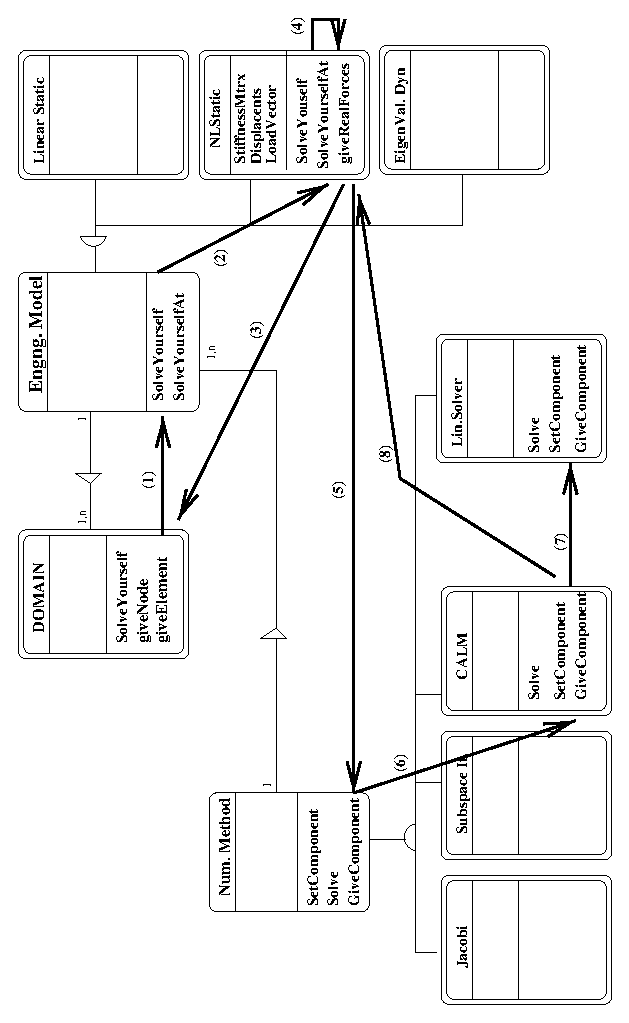
\includegraphics[width=0.7\textwidth]{struct2.eps}}
\end{htmlonly}
%begin{latexonly}
\ifpdf
\centerline{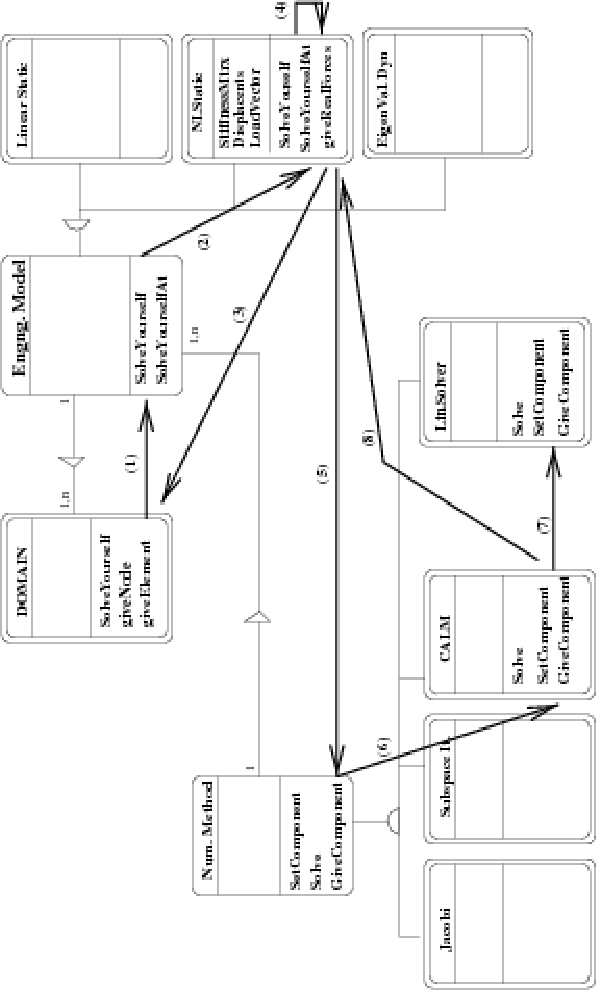
\includegraphics[angle=270,width=0.7\textwidth]{struct2.pdf}}
\else
\centerline{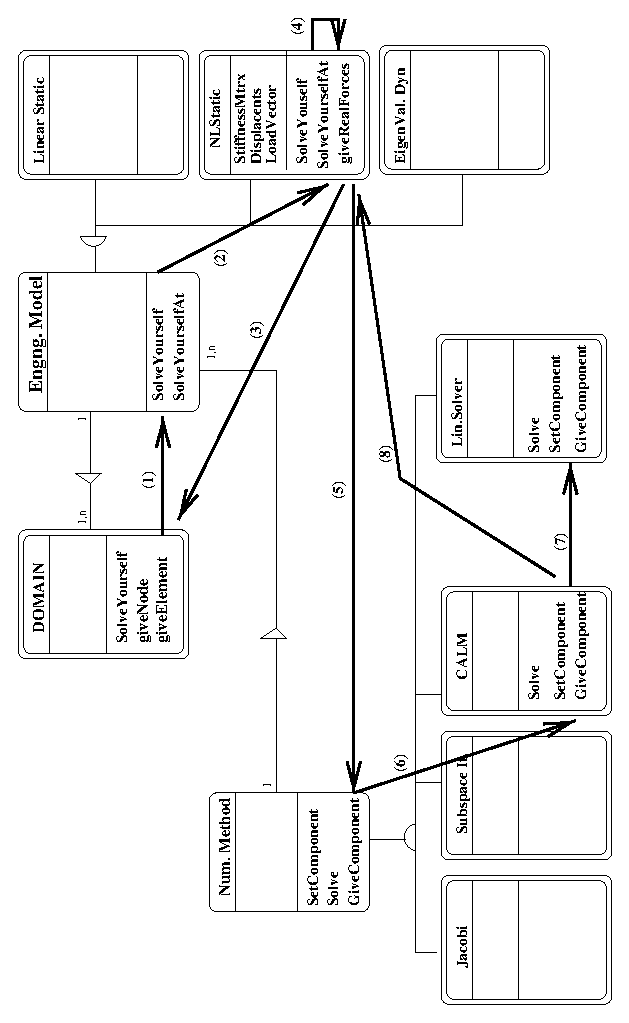
\includegraphics[angle=270,width=0.7\textwidth]{struct2.eps}}
\fi
%end{latexonly}
\caption{Engng model - Numerical method Interface.}
\label{engngNummet1fig}
\end{figure}



\begin{figure}[tb]
\begin{htmlonly}
  \htmlimage{thumbnail=0.9,flip=r270}
  \centerline{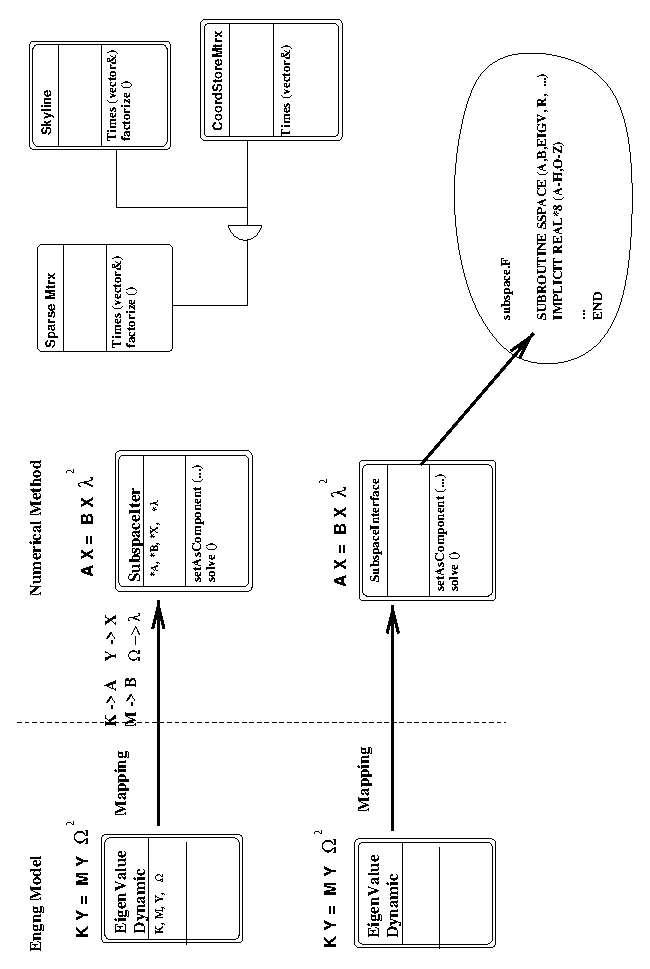
\includegraphics[width=0.7\textwidth]{engng.eps}}
\end{htmlonly}
%begin{latexonly}
\ifpdf
\centerline{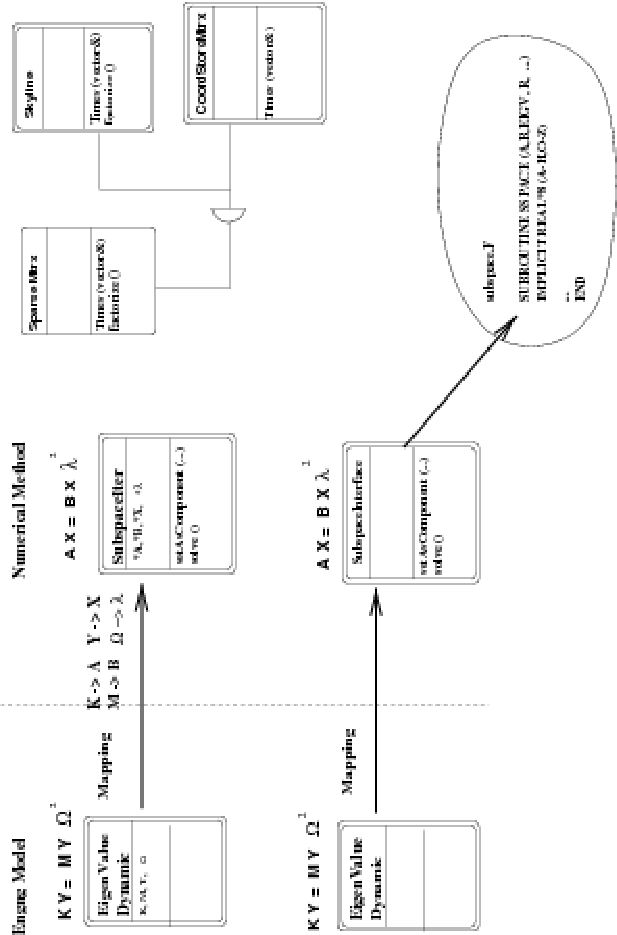
\includegraphics[angle=270,width=0.7\textwidth]{engng.pdf}}
\else
\centerline{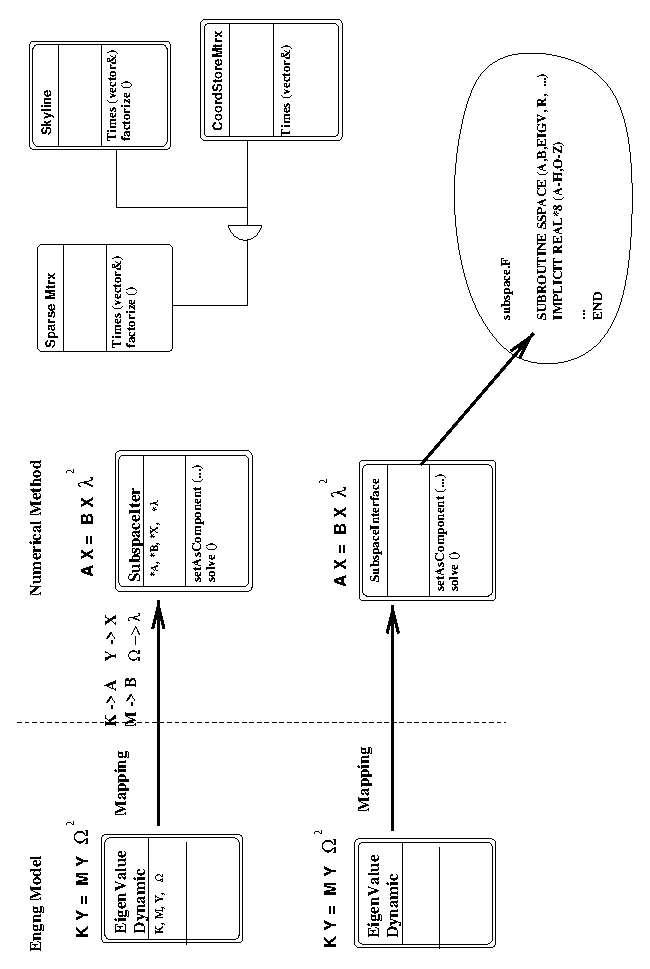
\includegraphics[angle=270,width=0.7\textwidth]{engng.eps}}
\fi
%end{latexonly}
\caption{Engng model - Numerical method Interface.}
\label{engngNummet2fig}
\end{figure}



%In this picture, you can see the interface of numerical method
%class. 
%Interface of Numerical method is schematically shown on fig. xx.
%Here, engng model represented by class eigen value dynamic,
%which as name indicates, represent dynamic eigen value problem. After
%it assembles its global stiffness and mass matrices, it creates
%suitable instance of  numerical method to solve the problem. Subspace
%iteration method has been selected here.

%\fig[t]{0mm\label{engngNummet1fig}\centerline{\epsfbox{struct2Sm.eps}}}           %obr.2
%{Engng model - Numerial method Interface}



The derived classes from \class{Numerical method} are supposed to
declare the interface for specific problem type
(like solution of linear system). The interface usualy consist in
declaring virtual abstract function solve, with parameters corresponding
to problem under consideration. The solve method shoud return
value of NM\_Status type. The data are specified using parameters passed to solve method (so called
mapping). (Other optional parameters can be provided via instanciateYourself
service, which receives the init record of corresponding metastep).

It should be pointed out, that all numerical methods solving the same
numerical problem use the same genaral interface (same mapping) - this is
enforced by using the same base problem-specific class. 
It is therefore possible to use any suitable
instance of the Numerical method class to solve the problem, and leave the  whole engineering model code,
including mapping, unchanged, because all instances of the Numerical
method class provide the common interface.

This concept is further enhanced by the introduction of a base abstract
class for all sparse matrices. This class only declares the basic
required services provided by all sparse matrices (like multiplication
by a vector, possible factorization, etc). The implementation is left on
derived classes.  Numerical methods are then implemented only
using basic services declared by the \class{Sparse Matrix} class. Thus, numerical
method class instances will work with any sparse matrix class, even
those added in the future, without changing any code, because all derived
classes of the \class{Sparse Matrix} class implement the same interface.

The declaration of \class{SparseLinearSystem} class (typical
problem-specific base class defining the interface for solving sparse
system of equations) is listed to
illustrate the basic concepts.
{\small\begin{verbatim}
//   **********************************
//   *** CLASS SparseLinearSystemNM ***
//   **********************************

 
#ifndef sparselinsystemnm_h


#include "nummet.h"
#include "cltypes.h"
#include "typeInfo.h"
#include <stdio.h>
class EngngModel ; class SparseMtrx; class FloatArray; 


/**
This base class is an abstraction for all numerical methods
solving sparse linear system of equations. 
The purpose of this class is to declare the general interface
to all numerical methods solving this kind of problem. 
This interface allows to use any suitable instance of the 
Numerical method class to the solve problem,
and leave the  whole engineering model code,
including mapping, unchanged, because all instances of this class
provide the common interface.
*/
class SparseLinearSystemNM : public NumericalMethod
{
protected:
public:
	/// Constructor
	SparseLinearSystemNM (int i, Domain* d,EngngModel* m);
	/// Destructor
	~SparseLinearSystemNM ();

	// identification 
	/// Returns class name of the receiver.
	char*  giveClassName (char* s) const 
	{ return strcpy(s,"SparseLinearSystemNM") ;}
	/** Returns classType id of receiver.
		@see FEMComponent::giveClassID 
		*/
	classType giveClassID () const { return SparseLinearSystemNMClass ;}

	/**
		Solves the given sparse linear system of equations Ax=b.
		@param A coefficient matrix 
		@param b right hand side
		@param x solution array
		@return NM_Status value
	 */
	virtual NM_Status solve (SparseMtrx* A, FloatArray* b, FloatArray* x) = 0;


 public:
 };

#define sparselinsystemnm_h
#endif
\end{verbatim}}

To summarize, the natural independence of the problem formulation,
numerical solution of the problem, and data storage format have been
obtained, which leads to a modular and extensible structure of the engineering
model - numerical method frame.

\subsection{Grid Representation - Domain}
The computational grid is represented by \class{Domain} class.
It stores all the components of the FEM model. These are dof managers
(nodes, element sides possessing DOFs), elements, material and cross
section models, boundary conditions
(primary boundary conditions as well as applied loading), and initial
conditions. For every component type the Domain maintains the
component list and provides the corresponding access services.
Domain keeps its number and link to associated problem (EngngModel).
It also keeps its domain type, which determines the default number of
Dofs per node (or side) and their physical meanings. Note, that this 
default setting can be redefined by particular nodes or sides.
The basic services provided by Domain are the following
\begin{itemize}
\item
Reading its description from input and creating corresponding objects.
This task includes the reading and parsing the particular mesh input
records, creating the corresponding components representations
(objects) of appropriate type, initializing these components using
theirs \service{instanciteFromString} methods and storing them into
corresponding list.
\item
Provides services for accessing its particular components. 
The services returning the total number of particular domain
components and particular component access methods based on component
number are provided. 
\end{itemize}
Domain also contains instance of \class{OutputManager} manager class,
which implements the output filtering capabilities. It allows to
filter output for specific solution steps, elements and dof managers.
The domain also can create (if needed) instances of
\class{SpatialLocalizer} class and \class{connectivityTable} class
to serve the connectivity and  spatial localization related services
(finding elements shared by the node, finding the closest node search,
finding the element containing given point, etc.).


\subsection{Example - Linear Static Analysis}
\label{Engngmodelexample}
In this section, the example of the implementation of linear static
analysis will be shown. The meta steps are not used, so the default
one is created. 
The class definition includes the declaration of characteristic
components of the problem - the stiffness matrix and load and
displacement vectors. Two additional variables are used to store the
solver type and the sparse matrix type, which can be selected by the user.
The services for solving the solution step (\service{solveYourselfAt}), 
requesting unknowns (\service{giveUnknownComponent}), context i/o
(\service{saveContext} and \service{restoreContext}), problem
initialization (\service{initializeFrom}), and  consistency checking
(\service{checkConsistency}) are overloaded.


{\small\begin{verbatim}
class LinearStatic : public StructuralEngngModel
{ 
/*
   This class implements LinearStatic Engineering problem.
 Multiple loading works only if linear elastic material (such as isoLE)  is used.
 (Other non-linear materials kepp load history, so such multiple loading
 will cause that next step will be assumed as new load increment, 
 not the total new load). Because they always copute real stresses acording
 to reached strain state, they are not able to respond to linear analysis.
  
DESCRIPTION:
   Solution of this problem is series of loading cases, maintained as sequence of
   time-steps. This solution is in form of linear equation system Ax=b
TASK:
   Creating Numerical method for solving Ax=b
   Interfacing Numerical method to Elements
   Managing time  steps
*/

 protected:
  SparseMtrx* stiffnessMatrix;
  FloatArray loadVector;
  FloatArray displacementVector;
  
  LinSystSolverType solverType;
  SparseMtrxType sparseMtrxType;
  /// Numerical method used to solve the problem
  SparseLinearSystemNM *nMethod;

  int initFlag;

#ifdef __PETSC_MODULE
  Vec _loadVec, _dispVec;
#endif

 public:
  LinearStatic (int i, EngngModel* _master = NULL) ;
  ~LinearStatic () 
    {delete  stiffnessMatrix; if (nMethod) delete nMethod;}
// solving
  void solveYourself ();
  void solveYourselfAt (TimeStep *);
  //int requiresNewLhs () {return 0;}
 /**
  Updates nodal values
  (calls also this->updateDofUnknownsDictionary for updating dofs unknowns dictionaries
  if model supports changes of static system). The element internal state update is also forced using
  updateInternalState service.
  */
  virtual void               updateYourself (TimeStep*) ;
  double   giveUnknownComponent ( EquationID, ValueModeType, TimeStep*, Domain*, Dof*);
  contextIOResultType saveContext (FILE* stream, void *obj = NULL) ;
  contextIOResultType restoreContext (FILE* stream, void *obj = NULL);

 void   updateDomainLinks();

  TimeStep* giveNextStep ();
  NumericalMethod* giveNumericalMethod (TimeStep*);
  //void printReactionForces (TimeStep *);
  void               terminate (TimeStep*);

 IRResultType initializeFrom (InputRecord* ir);

 // consistency check
 virtual int checkConsistency (); // returns nonzero if o.k.

  /** DOF printing routine. Called by DofManagers to print Dof specific part.
  Dof class provides component printing routines, but emodel is responsible
  for what will be printed at DOF level.
  @param stream output stream
  @param iDof dof to be processed
  @param atTime solution step
  */
 virtual void printDofOutputAt (FILE* stream, Dof* iDof, TimeStep* atTime);

// identification
  const char* giveClassName () const { return "LinearStatic";}
  classType giveClassID ()      const { return LinearStaticClass;}
  fMode giveFormulation () { return TL; }
#ifdef __PARALLEL_MODE
  /**
     Determines the space necessary for send/receive buffer.
     It uses related communication map pattern to determine the maximum size needed.
     @param commMap communication map used to send/receive messages
     @param buff communication buffer
     @return upper bound of space needed
  */
  int estimateMaxPackSize (IntArray& commMap, CommunicationBuffer& buff, int packUnpackType) ;
#endif
 
} ;
\end{verbatim}}

The listing of the \class{LinearStatic} class implementation follows. 
First, the \service{giveNumericalMethod} returns  the numerical method,
which will be used. The new instance is created if not defined
according to \attribute{nMethod} attribute, which is initialized from
input (see \service{instanciateYourself}). Note, that thanks to
the general interface, defined by the \class{NumericalMethod} class and the
component mapping approach, the further
communication with the numerical method uses only the interface declared by
the base \class{NumerialMethod} class and therefore there is no need to worry about
particular numerical method details. 
 
{\small\begin{verbatim}
NumericalMethod* LinearStatic :: giveNumericalMethod (TimeStep* atTime)
// only one has reason for LinearStatic 
//     - SolutionOfLinearEquations

{
  if (nMethod) return nMethod ;
	
	SparseLinearSystemNM* nm;
	if (solverType == ST_Direct) {
		nm = (SparseLinearSystemNM*) new LDLTFactorization (1,this->giveDomain(1),this);
		nMethod = nm;
		return nm;
	} else {
		nm = (SparseLinearSystemNM*) new IMLSolver (1,this->giveDomain(1),this);
		nMethod = nm;
		return nm;
	}
}

IRResultType
LinearStatic :: initializeFrom (InputRecord* ir)
{
  // Required by IR_GIVE_FIELD macro
  const char *__keyword, *__proc = "initializeFrom"; 
  IRResultType result;                              

  StructuralEngngModel::initializeFrom (ir);
  int val = 0;
  IR_GIVE_OPTIONAL_FIELD (ir, val, "lstype"); // Macro
  solverType = (LinSystSolverType) val;

  val = 0;
  IR_GIVE_OPTIONAL_FIELD (ir, val, "smtype"); // Macro
  sparseMtrxType = (SparseMtrxType) val;

  return IRRT_OK;
}
 


double LinearStatic ::  giveUnknownComponent (EquationID chc, ValueModeType mode, 
                TimeStep* tStep, Domain* d, Dof* dof)
// returns unknown quantity like displaacement, velocity of equation eq
// This function translates this request to numerical method language
{
 
 int eq = dof->giveEquationNumber();
 if (eq == 0) _error ("giveUnknownComponent: invalid equation number");

  if (tStep != this->giveCurrentStep ()) {
    _error ("giveUnknownComponent: unknown time step encountered");
  return 0.;
  }

  if (chc != EID_MomentumBalance) {
  _error ("giveUnknownComponent: Unknown is of undefined CharType for this problem");
  return 0.;
  }

  switch (mode)
   {
   case VM_Total:
   case VM_Incremental:
    if (displacementVector.isNotEmpty()) return displacementVector.at(eq);
    else return 0.;
    // return nMethod-> giveUnknownComponent (LinearEquationSolution, eq);

   default:
    _error ("giveUnknownComponent: Unknown is of undefined type for this problem");
   }
  return 0.;
}  


TimeStep* LinearStatic :: giveNextStep ()
{
  int istep = this->giveNumberOfFirstStep();
	//int mstep = 1;
  StateCounterType counter = 1;
	delete previousStep;

  if (currentStep != NULL) {
    istep =  currentStep->giveNumber() + 1   ;
		counter = currentStep->giveSolutionStateCounter() + 1;
	}
  previousStep = currentStep;
  currentStep = new TimeStep (istep,this, 1, (double) istep, 0., counter);
  // time and dt variables are set eq to 0 for staics - has no meaning
  return currentStep;
}

void  LinearStatic :: solveYourselfAt (TimeStep* tStep) {
//
// creates system of governing eq's and solves them at given time step
//
// first assemble problem at current time step

  if (initFlag) {

#ifdef VERBOSE
    OOFEM_LOG_INFO("Assembling stiffness matrix\n");
#endif
  
  //
  // first step  assemble stiffness Matrix
  //
  /*
    IntArray* mht = this -> GiveBanWidthVector ();
    stiffnessMatrix = new Skyline ();
    stiffnessMatrix ->  checkSizeTowardsBanWidth (mht) ;
    delete mht;
    */
  stiffnessMatrix = ::CreateUsrDefSparseMtrx(sparseMtrxType); // new Skyline ();
  if (stiffnessMatrix==NULL) _error ("solveYourselfAt: sparse matrix creation failed");
  //stiffnessMatrix = new DynCompCol ();
  //stiffnessMatrix = new CompCol ();
  
  stiffnessMatrix->buildInternalStructure (this, 1, EID_MomentumBalance);
  
  this -> assemble (stiffnessMatrix, tStep, EID_MomentumBalance, StiffnessMatrix, this->giveDomain(1));
  
  //
  // alocate space for displacementVector
  // 
  //displacementVector = new FloatArray (this->giveNumberOfEquations());
  displacementVector.resize (this->giveNumberOfEquations(EID_MomentumBalance));
  displacementVector.zero();

#ifdef __PETSC_MODULE
  if (solverType == ST_Petsc) {
    this->givePetscContext(1, EID_MomentumBalance)->createVecGlobal (&_loadVec);
    this->givePetscContext(1, EID_MomentumBalance)->createVecGlobal (&_dispVec);
  }
#endif
  initFlag = 0;
 }
#ifdef VERBOSE
  OOFEM_LOG_INFO("Assembling load\n");
#endif

#ifdef __PETSC_MODULE
  // direct interface to PETSC
  if (solverType == ST_Petsc) {
    this->petsc_assembleVectorFromElements(_loadVec, tStep, EID_MomentumBalance, 
                                           ElementForceLoadVector, VM_Total, 
                                           this->giveDomain(1));
    this->petsc_assembleVectorFromElements(_loadVec, tStep, EID_MomentumBalance, 
                                           ElementNonForceLoadVector, VM_Total, 
                                           this->giveDomain(1));
    this->petsc_assembleVectorFromDofManagers(_loadVec, tStep, EID_MomentumBalance, 
                                              NodalLoadVector, VM_Total, 
                                              this->giveDomain(1)) ;
    VecAssemblyBegin(_loadVec);
    VecAssemblyEnd (_loadVec);
   this->giveNumericalMethod(tStep);
#ifdef VERBOSE
    OOFEM_LOG_INFO("Solving ...\n");
#endif
    
    //nMethod -> solveYourselfAt(tStep);
    PetscSolver *ps = dynamic_cast<PetscSolver*>(nMethod);
    PetscSparseMtrx* psm = dynamic_cast<PetscSparseMtrx*>(stiffnessMatrix);
    ps -> petsc_solve (psm, _loadVec, _dispVec);
    
    this->givePetscContext(1, EID_MomentumBalance)->scatterG2N (_dispVec, &displacementVector, INSERT_VALUES); 
  } else 
#endif
  {
    // 
    // assembling the element part of load vector
    //
    //loadVector = new FloatArray (this->giveNumberOfEquations());
    loadVector.resize (this->giveNumberOfEquations(EID_MomentumBalance)); 
    loadVector.zero();
    
    this->assembleVectorFromElements(loadVector, tStep, EID_MomentumBalance, 
                                     ElementForceLoadVector, VM_Total, this->giveDomain(1));
    this->assembleVectorFromElements(loadVector, tStep, EID_MomentumBalance, 
                                     ElementNonForceLoadVector, VM_Total, this->giveDomain(1));
    
    // 
    // assembling the nodal part of load vector
    //
    this->assembleVectorFromDofManagers(loadVector, tStep, EID_MomentumBalance, 
                                        NodalLoadVector, VM_Total, this->giveDomain(1)) ;
    
    //
    // set-up numerical model
    //
    this->giveNumericalMethod(tStep);
    
    /*
      nMethod -> setSparseMtrxAsComponent ( LinearEquationLhs , stiffnessMatrix) ; 
      nMethod -> setFloatArrayAsComponent ( LinearEquationRhs , &loadVector) ; 
      nMethod -> setFloatArrayAsComponent ( LinearEquationSolution, &displacementVector) ;
    */
    // 
    // call numerical model to solve arised problem
    //
#ifdef VERBOSE
    OOFEM_LOG_INFO("Solving ...\n");
#endif
    
    //nMethod -> solveYourselfAt(tStep);
    nMethod -> solve (stiffnessMatrix, &loadVector, &displacementVector);
  }
  tStep->incrementStateCounter();              // update solution state counter
  //
  // update nodes, elements, etc.
  this->updateYourself(this->giveCurrentStep());
  
} 


void    LinearStatic :: updateYourself (TimeStep* stepN) 
{
	this->updateInternalState(stepN);
	StructuralEngngModel::updateYourself(stepN);
}


contextIOResultType LinearStatic :: saveContext (FILE* stream, void *obj)
// 
// saves state variable - displacement vector
//
{
	contextIOResultType iores;
	int closeFlag = 0;

	if (stream==NULL) {
		if (!this->giveContextFile(&stream,this->giveCurrentStep()->giveNumber(),
	                             contextMode_write)) 
			THROW_CIOERR(CIO_IOERR); // override 
		closeFlag = 1;
	}

  if ((iores = StructuralEngngModel :: saveContext (stream)) != CIO_OK) 
      THROW_CIOERR(iores);
  if ((iores = displacementVector.storeYourself(stream)) != CIO_OK) 
      THROW_CIOERR(iores);

	if (closeFlag) fclose (stream); // ensure consistent records
  return CIO_OK;
}



contextIOResultType LinearStatic :: restoreContext (FILE* stream, void *obj)
// 
// restore state variable - displacement vector
//
{
	contextIOResultType iores;
	int closeFlag = 0;
	int istep = this->resolveCorrespondingStepNumber (obj);

	if (stream == NULL) {
		if (!this->giveContextFile(&stream, istep, contextMode_read))
			THROW_CIOERR(CIO_IOERR); // override 
		closeFlag = 1;
	}

	if ((iores=StructuralEngngModel::restoreContext(stream,obj))!=CIO_OK)
     THROW_CIOERR(iores);
	if ((iores=displacementVector.restoreYourself(stream))!=CIO_OK)
      THROW_CIOERR(iores);

	
  if (closeFlag) fclose (stream); // ensure consistent records
	return CIO_OK;
}





void
LinearStatic:: terminate(TimeStep* tStep)
{
	StructuralEngngModel :: terminate (tStep);
	this->printReactionForces (tStep, 1);
}



int
LinearStatic::checkConsistency ()
{
// check internal consistency
// if success returns nonzero
	int i, nelem;
	Element* ePtr;
	StructuralElement* sePtr;
	Domain* domain = this->giveDomain(1);

	nelem = domain->giveNumberOfElements();
	// check for proper element type

	for (i=1; i<= nelem; i++) {
		ePtr = domain->giveElement(i);
		sePtr = DYNAMIC_CAST (StructuralElement, ePtr);
		if (sePtr == NULL) {
			printf ("Error: Element %d has no StructuralElement base\n",i);
			return 0;
		}
	}

	EngngModel :: checkConsistency ();

	return 1;
}


void
LinearStatic::updateDomainLinks ()
{
 EngngModel::updateDomainLinks();
	this->giveNumericalMethod(giveCurrentStep())->setDomain (this->giveDomain(1));
}
\end{verbatim}}

%\subsection {Program \& Data Flow}
%%(slide frame 3 - program flow engng model - numerical method)
%The program flow in the engineering model --- numerical method frame is 
%explained in Fig.~3. After \class{Domain} reads the input file with
%the problem description,
%it starts computation by invoking \service{SolveYourself} service of \class{Engng
%model} class. In this example a non-linear static problem
%analysis is performed. The corresponding \class{Engng model} class solves the whole problem
%as a series of load increments. Therefore, for each step of computation,
%a \service{SolveYourselfAt} service is invoked. For the first step, the reference
%load vector is formed from element and nodal contributions, so these
%components are accessed from corresponding domain using its
%services. Then, for each solution step,  the stiffness matrix is formed
%and particular components of the governing equation are mapped to
%the numerical method components. Here, an \class{CALM} instance of \class{Numerical
%Method} class is being used. For solution of a linearized problem, the
%\class{CALM} uses another instance of \class{Numerical method} class - here named
%\class{Linear solver}. After components are mapped and a solution is obtained,
%the \class{CALM} checks convergence. It asks \class{Engng model} to compute
%(update) the vector of real nodal forces according to the solution reached,
%and checks convergence. If convergence is reached, the program control
%returns to \class{Engng model} and the solution step is then terminated (stress
%updates and necessary printing) and the solution continues with next
%step. If prescribed accuracy is not reached, the stiffness matrix can be
%updated by suitable engng model service and iteration continues. 


%\fig[t]{0mm\label{engngNummet2fig}\centerline{\epsfbox{engng-nummet2Sm.eps}}}           %obr.4
%{General Structure}


\section{Material --- Element Frame}
\label{materialEleemntFrame}
As already mentioned, in Fig.~2 the material-element
frame is schematically shown.
In this frame, the following base classes \&
objects are introduced:


\begin{itemize}
\item
Class \class{Element}, which is an abstraction of a finite element. It declares
common general services, provided by all elements. Derived
classes are the base classes for specific analysis types (structural
analysis, thermal analysis).  They declare and implement necessary services for
specific analysis.

\item
\class{Integration point} class \& object: It is an abstraction for
the integration
point of the finite element. It maintains its coordinates and integration
weight. Any integration point can generally contain any number of
other integration points - called slaves. The \class{Integration
point} containing slaves is called master. Slaves are, for example,
introduced by a layered cross section model, where they represent
integration points for each layer, or can be introduced at material
model level, where they may represent, for example, micro-planes. Slave
integration points are hidden from elements. The \class{Integration point}
also contains associated material status (the reasons for introducing
this feature will be explained later).

\item
\class{Cross section} class is an abstraction for cross section. Its
main role is to hide from an element all details concerning the cross
section description and implementation. By cross section description
is meant, for example, an integral cross section model, layered cross
section model or fibered model. Elements do not communicate directly
with material, instead they always use a \class{Cross Section} interface, which
performs all necessary integration over its volume and invokes
necessary material class services\footnote{For some problems, the use
of cross section is not necessary, and then
the elements can communicate directly with material model. However, for
 some problems (for example structural analysis) the introduction of cross section 
is natural.}. The \class{Cross section} interface, defined in
terms of general functions, allows the use of any cross section
model, even that added in the future, without modification of any code,
because all cross section models implement the same interface.


\item
\class{Material} class is shown here. It represents base class for all
constitutive models. Derived classes should be the base
analysis-specific classes, which declare required analysis
specific services (for example structural material class declares
services for the stiffness computation and services for the real stress
evaluation). Again, the material analysis specific interface, defined
in terms of general services, allows the use of any material model, even
that added in the future, without modifying any code, because all material
models implement the same interface.
\end{itemize}

One of the most important goals, which have been formulated, is
extensibility. In the case of extension of the material library, the
analyst is facing  a key problem. Every material model must store
its unique history parameters for every related integration point. The
amount, type, and meaning of these history variables vary for each
material model. Therefore, it is not possible to efficiently
match all needs and to reflect them in the integration point data
structure. The suggested remedy is the following:

The \class{Integration point}  class is equipped with the possibility to have
associated a \class{Material status} class. When a new material model is
implemented, the analyst has also to declare and implement a related
material status derived from the base
\class{Material status} class to this material model. This status contains all necessary
history variables and data access and modification
services. The \class{Integration point} provides services for inserting and
accessing its related status. For every  \class{Integration point},
the corresponding material creates unique copy of its related material
status and associates it with that integration point. Because
the \class{Integration point} is a compulsory parameter of all messages sent to
any material model, the particular material model can access its
related material status from the given \class{Integration point}, and therefore can access its
history variables. 


%%\section{General Material Interface}
%%(slide General Material interface - frame 1)

%\fig[t]{0mm\label{materelementFrame1}\centerline{\epsfbox{struct1Sm.eps}}}           %obr.1
%{General Structure}

\begin{figure}[tb]
\begin{htmlonly}
  \htmlimage{thumbnail=0.9,flip=r270}
  \centerline{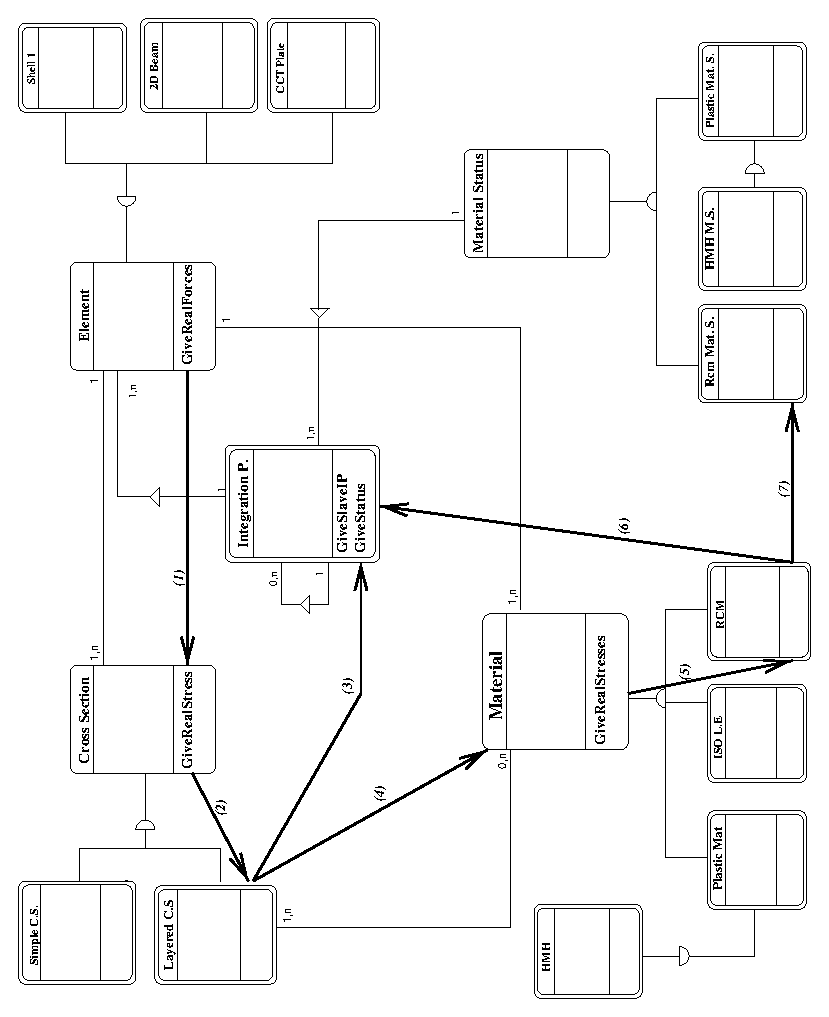
\includegraphics[width=0.7\textwidth]{struct1.eps}}
\end{htmlonly}
%begin{latexonly}
\ifpdf
\centerline{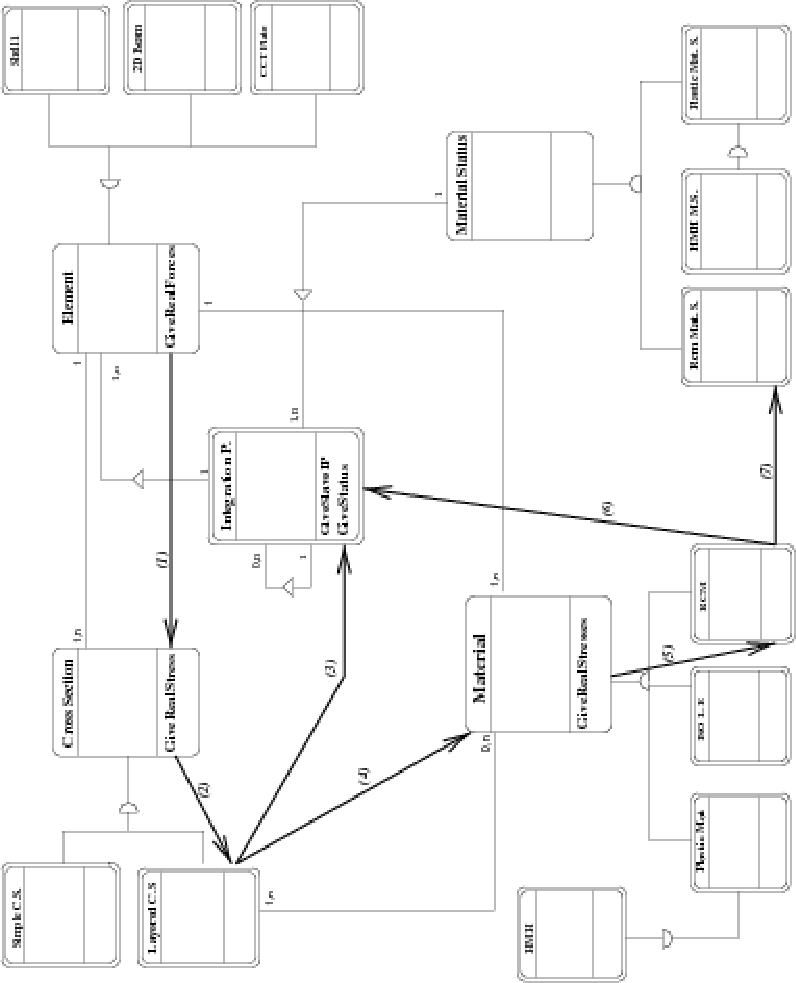
\includegraphics[angle=270, width=0.7\textwidth]{struct1.pdf}}
\else
\centerline{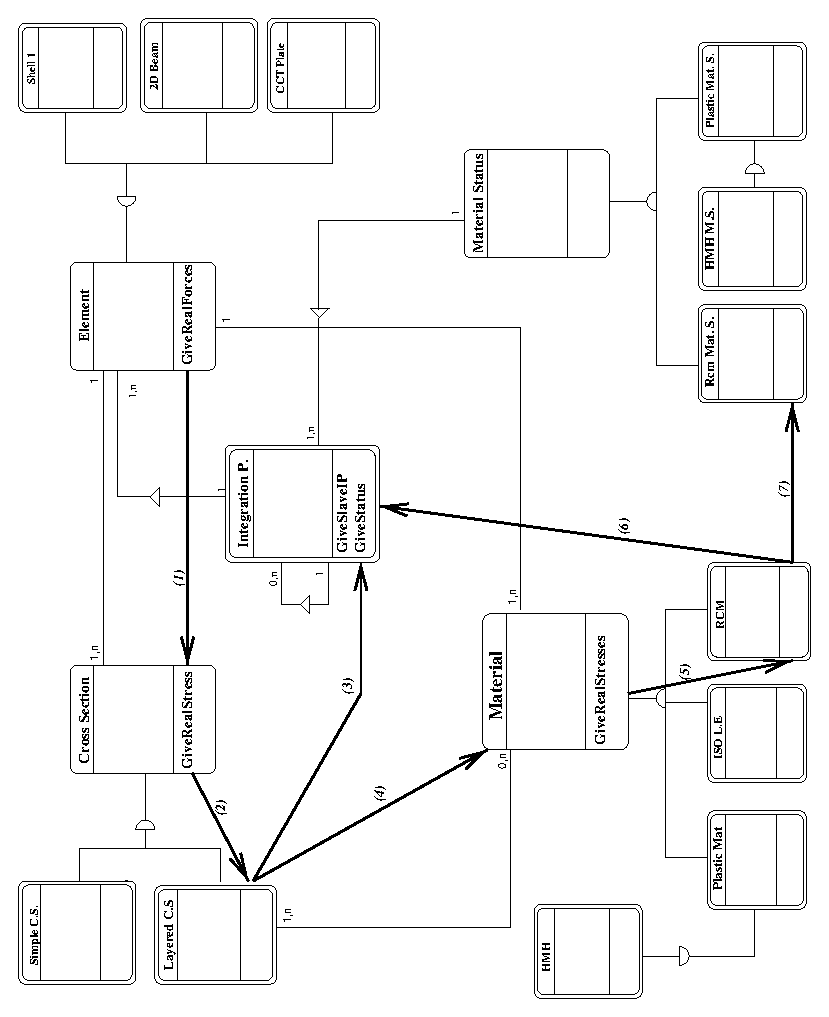
\includegraphics[angle=270, width=0.7\textwidth]{struct1.eps}}
\fi
%end{latexonly}
\caption{Element-material frame  structure.}
\label{materelementFrame1}
\end{figure}


In Fig.~\ref{materelementFrame1}, the material - element frame is
depicted in more detail, although it is still simplified. A simple cross
section model class hierarchy is shown there. There are two 
derived classes from the parent \class{Cross Section} class: \class{Simple cross section}
class representing an integral cross section model and \class{Layered cross
section model} class, representing a layered cross section model
implementation. At the bottom,  the hierarchies of the material model and
the associated material status representations are indicated.
The program flow for an element, requesting the computation of its real nodal forces is also
indicated in Fig.~\ref{materelementFrame1}. This is generally done by integrating real stresses at its integration
points. For each \class{Integration point} it asks the \class{Cross section} model to
compute real stresses at the given integration point. In this example,
the \class{Layered cross section} uses the master-slave integration point
principle. Each element integration point, here called master,
contains its slaves, each representing one layer. These slave
integration points are introduced by the cross section model, and are
hidden to the element. For a given master integration point, the cross section
model performs integration  over cross section
volume using slaves. Therefore  each slave integration point, which is requested
by the master, uses material model class services to compute real
stresses for each corresponding layer, passing the slave integration point as
a parameter. Then for each slave, the material model asks the given integration
point for its associated status.  Having obtained reference to it,
the material model can access all its history variables through status
services, and computes results.

\subsection{Base Element class}
This class is the base class for all FE elements. It is also the
abstract class, declaring some services, which have to be implemented
by the derived classes. The main purpose of this class is to serve the
basic common services, which are common to all finite elements (like
storing the references to element's material model, nodes and applied
loadings, assembling location array, storing
from/to context file, etc.). The \class{Element} class does neither declare nor
implement any method related to specific analysis. These services are to be declared
and possibly implemented by derived classes.\footnote{
When a specific services are required at element level by other
components of a system (error estimator, graphics subsystem, etc.)
they can be included using so-called interface concept at particular
element level using  multiple inheritance.} These derived classes
(direct children of \class{Element} class) are therefore assumed to be base
classes for particular analysis or problem type, represented by
corresponding engng model. They typically
declare the general services required for a specific analysis purpose
- like evaluation of stiffness or mass matrices for structural
analysis, or evaluation of capacity and conductivity matrices for heat
transfer analysis. Usually they also provide general implementation of
these services.

The \class{Element} is derived from a \class{FEMComponent}. It inherits
the \class{FEMComponent}'s ability to keep its number and reference
to the domain, it belongs to, its error and warning
reporting services, methods for field extraction functions from object
record (used when element reads its description from input database).
Also the \class{FEMComponent} declares several abstract services. The most
important are \service{initializeFrom} for object
initialization from a given record, \service{saveContext} and
\service{restoreContext} methods for storing and restoring object state
to/from a stream, and \service{giveInterface} service for requesting
an object interface.

The attributes declared at the \class{Element} class include the 
variables used to keep its list of nodes and sides, its material
and cross section number, lists of applied body and boundary loads,
list of integration rules and array storing its code numbers
(see \refman for details).


The following important services are declared at the element level:
\begin{itemize}
\item services for component management - include services for
requesting element's geometrical characteristics
(\service{giveDofManager}, \service{giveNode},
\service{giveNumberOfDofManagers},
\service{giveNumberOfNodes}), material (\service{giveMaterial}), cross
section (\service{giveCrossSection}).

\item services related to code numbers management:\\
\service{giveLocationArray} - returns the element location array. This
location array is obtained by appending  code-numbers of element
nodes (according to the node numbering), followed by code numbers of
element sides. The ordering of DOFs for the particular node/side is
specified using a node/side DOF mask, which is obtained using
\service{giveNodeDofIDMask} or \service{giveSideDofIDMask} services.
Please note, that this local DOF ordering must be taken into account when assembling various local characteristic 
  vectors and matrices. Once the element location array is assembled,
it is cached and reused to avoid time consuming assembly. 
 Some engineering models
  may support dynamic changes of the static system (generally, of boundary conditions) during analysis,
  then these models use \service{invalidateLocationArray} function to invalidate location array
after finishing time step, to force new equation numbering.\\
\service{computeNumberOfDofs} - computes or simply returns total
number of element's local DOFs. Must be implemented by particular
element. The \service{giveDofManDofIDMask} service return
DOF mask for corresponding dof manager (node or side). This mask defines the DOFs which are used by element 
at the given node/side. The mask influences the code number ordering
for the particular node. Code numbers are 
ordered according to the node order and DOFs belonging to the particular node are ordered 
according to this mask. If element requests DOFs using a node mask
which are not in the node
then error is generated. This masking allows node to be shared by different elements with 
different DOFs in the same node/side. Element's local code numbers are
extracted from the node/side using 
this mask. These services must be implemented (overloaded) by
particular element implementations.
\item
services for requesting the so-called  characteristic
components. (\service{giveCharacteristicMatrix} and
\service{giveCharacteristicVector}). 
The component requested is identified by parameter of type
``CharType'' (see cltypes.h). These are general methods for obtaining various element
contributions to the global problem. These member functions have to
be overloaded by derived analysis-specific 
classes in order to invoke the proper method according to the type of
requested component.
\item
services related to the solution step update and termination.\\
These services are used to update the internal variables at
element's integration points prior to reached state
(\service{updateYourself} and \service{updateInternalState}).
Similar service for the internal state initialization is also declared
(see \service{initializeYourself}) and re-initialization to previous
equilibrium state (see \service{initForNewStep}).
\item
services for accessing local element's unknowns from corresponding DOFs.
These include methods for requesting local element vector of unknowns
(\service{computeVectorOf}) and local element vector of prescribed
unknowns (\service{computeVectorOfPrescribed}).
\item
Services for handling transformations between element local coordinate
system and coordinate system used in nodes (possibly different from
global coordinate system).  
\item
miscellaneous services. Their detailed description can be found in
\refman (see also \file{element.h} (declaration) and
\file{element.C} (implementation) files).

\end{itemize}

\subsection{Analysis specific element classes}
The direct child classes of the \class{Element} class are assumed to be base
classes for particular analyses. For example, the
\class{StructuralElement} class is the base class for all ``structural''
elements. It declares all necessary services required by structural
analysis (for example methods computing stiffness  matrices, load,
strain and stress  vectors etc.). This class may provide general
implementations of some of these services if possible, implemented
by virtual functions (they reflect specific element formulation
- like computing element shape functions), which are declared, but
their implementation is left on derived classes, which implement specific
elements.

\subsubsection{Structural Element -  Example}
This class is the base class for all structural elements.
It is derived from the \class{Element} class. 
The basic tasks of the structural element is to compute its contributions
to global equilibrium equations (mass and stiffness matrices, various
load vectors (due to boundary conditions, force loading, thermal
loading, etc.) and computing the corresponding strains and stresses
from nodal displacements. Therefore the corresponding virtual services
for computing these contributions are declared.
These standard contributions can be computed by numerical
integration  of appropriate terms, which typically depend on 
element interpolation or material model, over the element volume. Therefore, it is possible to
provide general implementations of these services, provided that the
corresponding methods for computing interpolation dependent terms and
material terms are implemented, and corresponding integration rules
are initialized. 
This concept will be demonstrated on service computing stiffness
matrix. Since element stiffness matrix contributes to the global
equilibrium, the stiffness will be requested using
\service{giveCharacteristicMatrix} service. 
The implementation of the services of the structural element takes
into account only material nonlinearity, the geometrical nonlinearity 
is not taken into account (regarding geometrical nonlinearity, see \class{NLStructuralElement} class).
The implementation of this
service is following:
\begin{verbatim}
void
StructuralElement ::  giveCharacteristicMatrix (FloatMatrix& answer, 
                      CharType mtrx, TimeStep *tStep) 
// 
// returns characteristic matrix of receiver according to mtrx
//
{
  if (mtrx == TangentStiffnessMatrix) 
    this -> computeStiffnessMatrix(answer, TangentStiffness, tStep);
  else if (mtrx == SecantStiffnessMatrix) 
    this -> computeStiffnessMatrix(answer, SecantStiffness, tStep);
  else if (mtrx == MassMatrix) 
    this -> computeMassMatrix(answer, tStep);
  else if 
  ....
}
\end{verbatim}
The first parameter is the matrix object to be computed, the mtrx
parameter determines the type of contribution and the last parameter, time step, represents time.
The element stiffness matrix can be evaluated using
$$
\mbf{K} = \int_{V} \mbf{B}^T\mbf{D}\mbf{B}\;dV,
$$
where $\mbf{B}$ is the so-called geometrical matrix, containing
derivatives of shape functions and $\mbf{D}$ is the material stiffness
matrix. If $\mbf{D}$ is symmetric (which is usually the case) then
element stiffness is symmetric, too. The numerical integration is used to evaluate this integral.
For numerical integration, the  \class{IntegrationRule} class is used.
The integration rules for a specific element are created during element
initialization and are stored in \attribute{integrationRulesArray} attribute,
inherited from the \class{Element} class. In order to implement the stiffness
evaluation, the methods for computing geometrical matrix and material stiffness
matrix are declared (as virtual), but not implemented. They have to
be implemented by specific elements, because they ``know'' their interpolation
and the corresponding material mode. 
The implementation of
\service{computeStiffnessMatrix} is following
\begin{verbatim}
void
StructuralElement :: computeStiffnessMatrix (FloatMatrix& answer, 
                     MatResponseMode rMode, TimeStep* tStep)
// Computes numerically the stiffness matrix of the receiver.
{
  int j;
  double      dV ;
  FloatMatrix d, bj, dbj;
  GaussPoint  *gp ;
  IntegrationRule* iRule;

  // give reference to integration rule
  iRule = integrationRulesArray[giveDefaultIntegrationRule()];
     
  // loop over integration points
  for (j=0 ; j < iRule->getNumberOfIntegrationPoints() ; j++) {
     gp = iRule->getIntegrationPoint(j) ;
     // compute geometrical matrix of particular element 
     this -> computeBmatrixAt(gp, bj) ;  
     //compute material stiffness
     this -> computeConstitutiveMatrixAt(d, rMode, gp, tStep); 
     // compute jacobian
     dV = this -> computeVolumeAround(gp) ; 
     // evaluate stiffness
     dbj.beProductOf (d, bj) ;
     answer.plusProductSymmUpper(bj,dbj,dV) ; 

  }
 
  answer.symmetrized() ;
  // transform into global coordinate system if necessary
  if (this->updateRotationMatrix()) 
     answer.rotatedWith(*this->rotationMatrix) ;
  return  ;
}
\end{verbatim}
Inside the integration loop, only the upper half of the element stiffness is
computed in element local coordinate system. Then, the lower part of 
the stiffness is initialized from the upper part (answer.symmetrized()) and
transformation from element local coordinate system to global
coordinate system is done. The transformation matrix is cached in
the \attribute{rotationMatrix} attribute declared in the \class{StructuraleElement} class. 
The \service{updateRotationMatrix} service
updates this matrix (if necessary) and returns pointer to this matrix.
The zero value indicates that no transformation is necessary. 
The other element contributions can be computed using similar
procedures. In general, different integration rules can be used for
evaluation of different element contributions. For example, the
support for the reduced
integration of some terms of the stiffness matrix can be implemented - see
the implementation of \service{computeStiffnessMatrix} in \file{structuralelement.C}.

The element strain and stress vectors at a given integration point are
computed using \service{computeStrainVector} and
\service{computeStressVector} services. The element strain vector can
be evaluated using $\mbf{\varepsilon}=\mbf{B}\mbf{u}$, where $\mbf{B}$
is the geometrical matrix and $\mbf{u}$ is element local displacement
vector. The stress evaluation is rather simple, since the stress
evaluation from a given strain increment and actual state (kept within
the integration point) is done at the cross section description level
(integration over cross section volume) and material model level
(stress evaluation).
\begin{verbatim}
void
StructuralElement :: computeStrainVector (FloatArray& answer, 
                     GaussPoint* gp, TimeStep* stepN)
// Computes the vector containing the strains 
// at the Gauss point gp of the receiver, 
// at time step stepN. The nature of these strains depends
// on the element's type.
{
  FloatMatrix b;
  FloatArray  u ;
  
  this -> computeBmatrixAt(gp, b) ;
  // compute vector of element's unknowns
  this -> computeVectorOf(DisplacementVector,
                          UnknownMode_Total,stepN,u) ;
  // transform global unknowns into element local c.s.
  if (this->updateRotationMatrix()) 
     u.rotatedWith(this->rotationMatrix,'n') ;
  answer.beProductOf (b, u) ;
  
  return ;
}


void
StructuralElement :: computeStressVector (FloatArray& answer, 
                     GaussPoint* gp, TimeStep* stepN)
// Computes the vector containing the stresses 
// at the Gauss point gp of the receiver, at time step stepN. 
// The nature of these stresses depends on the element's type.
{

  FloatArray Epsilon ;
  StructuralCrossSection* cs = (StructuralCrossSection*) 
                                this->giveCrossSection();
  Material *mat = this->giveMaterial();
  
  this->computeStrainVector (Epsilon, gp,stepN) ;
  // ask cross section model for real stresses 
  // for given strain increment 
  cs -> giveRealStresses (answer, ReducedForm, gp, Epsilon, stepN);

  return  ;
}
\end{verbatim}

The \class{StructuralElement} class overloads also services for
context storing/restoring, calling corresponding services for all
integration rules (and thus on all integration points belonging to
an element). 

For further reference see \refman and files \file{structuralelement.h}
and \file{structuralelement.C}.

\subsubsection{Isoparametric Truss 2d element}

\begin{verbatim}
class Truss2d : public StructuralElement
{
/*
 This class implements a two-node truss bar element 
 for two-dimensional analysis.
 A truss bar element is characterized by its 'length' 
 and its 'pitch'. The pitch is the angle in radians 
  between the X-axis anf the axis of the element 
  (oriented node1 to node2).
 */

 protected :
   double        length ;
   double        pitch ;

 public :
   Truss2d (int,Domain*) ;    // constructor
   ~Truss2d ()   {}           // destructor

   // mass matrix coputations
   void computeLumpedMassMatrix (FloatMatrix& answer, 
                                 TimeStep* tStep) ;
   // general mass service overloaded 
   void computeMassMatrix (FloatMatrix& answer, TimeStep* tStep) 
        {computeLumpedMassMatrix(answer, tStep);}

       // DOF management
   virtual int            computeNumberOfDofs (EquationID ut) {return 4;}
   virtual void           giveDofManDofIDMask  (int inode, EquationID, IntArray& ) const;

       double computeVolumeAround (GaussPoint*) ;

 // 
 // definition & identification
 //
   char* giveClassName (char* s) const 
         { return strcpy(s,"Truss2d") ;}
   classType giveClassID () const { return Truss2dClass; } 

   IRResultType initializeFrom (InputRecord* ir);

 protected:
   // computes geometrical matrix 
   void computeBmatrixAt (GaussPoint*, FloatMatrix&, 
                          int=1, int=ALL_STRAINS) ;
   // computes interpolation matrix
   void computeNmatrixAt (GaussPoint*, FloatMatrix&) ;
   // initialize element's integration rules
   void computeGaussPoints () ;
   // transformation from global->local c.s.
   int           computeGtoLRotationMatrix (FloatMatrix&);

   double giveLength () ;
   double givePitch () ;
 } ;

 \end{verbatim}
 This is a minimal-functionality implementation. It does not include,
 for example, any support for element loading or material
 nonlinearity.  The implementation starts with standard constructor and
 destructor.
 \begin{verbatim}

 Truss2d :: Truss2d (int n, Domain* aDomain) : 
            StructuralElement (n,aDomain)
 // Constructor.
 {
    numberOfDofMans       = 2 ;
    rotationMatrix      = NULL ;
    length              = 0. ;
    pitch               = 10. ;      // a dummy value

 }

 \end{verbatim}

 Next, the services for computing interpolation and geometrical matrices
 follow. The implementation of the \service{computeNmatrixAt}  is not necessary
 for the current purpose, since the mass matrix computation is overloaded
 and does not require this service, but it is added for completeness.
 The both methods compute response at a given integration point, which is
 passed as a parameter. The \service{computeBmatrixAt} has two additional
 parameters which determine the range of strain components for which
 response is assembled. This has something to do with support for
 reduced/selective integration and is not important in presented simple case.

 Recently, the interpolation classes have been added, that can significantly facilitate the element implementation. They provide shape functions, their derivatives, transformation jacobians out of the box. 
 \begin{verbatim}
 void
 Truss2d :: computeNmatrixAt (GaussPoint* aGaussPoint, 
                              FloatMatrix& answer) 
 // Returns the displacement interpolation matrix {N} 
 // of the receiver, evaluated at aGaussPoint.
 {
    double       ksi,n1,n2 ;

    ksi = aGaussPoint -> giveCoordinate(1) ;
    n1  = (1. - ksi) * 0.5 ;
    n2  = (1. + ksi) * 0.5 ;

    answer.resize (2,4);
    answer.zero();

    answer.at(1,1) = n1 ;
    answer.at(1,3) = n2 ;
    answer.at(2,2) = n1 ;
    answer.at(2,4) = n2 ;

    return  ;
 }


 void
 Truss2d :: computeBmatrixAt (GaussPoint* aGaussPoint, 
                              FloatMatrix& answer, int li, int ui)
 // 
 // Returns linear part of geometrical 
 // equations of the receiver at gp.
 // Returns the linear part of the B matrix
 //
 {
   double coeff,l;

   answer.resize(1,4);
   l = this->giveLength();
   coeff = 1.0/l;

   answer.at(1,1) =-coeff;
   answer.at(1,2) = 0.0;
   answer.at(1,3) = coeff;
   answer.at(1,4) = 0.0;

   return;
 }
 \end{verbatim}

 The following two functions compute the basic geometric
 characteristics of a bar element - its length and pitch, defined as the
 angle between global x-axis and the local element x-axis (oriented
 from node1 to node2).

 \begin{verbatim}

 double  Truss2d :: giveLength ()
    // Returns the length of the receiver.
 {
    double dx,dz ;
    Node   *nodeA,*nodeB ;

    if (length == 0.) {
       nodeA = this->giveNode(1) ;
       nodeB = this->giveNode(2) ;
       dx    = nodeB->giveCoordinate(1)-nodeA->giveCoordinate(1);
       dz    = nodeB->giveCoordinate(3)-nodeA->giveCoordinate(3);
       length= sqrt(dx*dx + dz*dz) ;}

    return length ;
 }


 double  Truss2d :: givePitch ()
    // Returns the pitch of the receiver.
 {
    double xA,xB,zA,zB ;
    Node   *nodeA,*nodeB ;

    if (pitch == 10.) {  // 10. : dummy initialization value
       nodeA  = this -> giveNode(1) ;
       nodeB  = this -> giveNode(2) ;
       xA     = nodeA->giveCoordinate(1) ;
       xB     = nodeB->giveCoordinate(1) ;
       zA     = nodeA->giveCoordinate(3) ;
       zB     = nodeB->giveCoordinate(3) ;
       pitch  = atan2(zB-zA,xB-xA) ;}

    return pitch ;
 }

 \end{verbatim}

 When an element is created (by the \class{Domain} class), the default
 constructor is called. To initialize the element, according to its
 record in the input database, the \service{initializeFrom} is
 immediately called after element creation. The element implementation
 should first call the parent implementation to ensure that attributes
 declared at parent level are initialized properly. Then the element has to
 initialize attributes declared by itself and also to set up its
 integration rules. In our example, special method
 \service{computeGaussPoints} is called to
 initialize integration rules.
 In this case, only one integration rule is created. It is of type 
 \class{GaussIntegrationRule}, indicating that the Gaussian  integration
 is used. Once integration rule is created, its integration points are 
 created to represent line integral, with 1 integration
 point. Integration points will be associated to element under
 consideration and will have 1D material mode (which determines the type of
 material model response).
 \begin{verbatim}
 IRResultType
 Truss2d :: initializeFrom (InputRecord* ir)
 {
    this->NLStructuralElement :: initializeFrom (ir);
    this -> computeGaussPoints();
    return IRRT_OK;
 }

 void  Truss2d :: computeGaussPoints ()
    // Sets up the array of Gauss Points of the receiver.
 {

  numberOfIntegrationRules = 1 ;
  integrationRulesArray = new IntegrationRule*;
  integrationRulesArray[0] = new GaussIntegrationRule (1,domain, 1, 2);
  integrationRulesArray[0]->
    setUpIntegrationPoints (_Line, 1, this, _1dMat);

 }

 double  Truss2d :: computeVolumeAround (GaussPoint* aGaussPoint)
 // Returns the volume corresponding to given integration point. 
 {
   double weight  = aGaussPoint -> giveWeight() ;
   return 0.5 * this->giveLength() * weight * 
          this->giveCrossSection()->give('A');
 }
 \end{verbatim}


 \begin{verbatim}
 void
 Truss2d :: computeLumpedMassMatrix (FloatMatrix& answer, TimeStep* tStep)
    // Returns the lumped mass matrix of the receiver. This expression is
    // valid in both local and global axes.
 {
    Material* mat ;
    double    halfMass ;

    mat        = this -> giveMaterial() ;
    halfMass   = mat->give('d') * 
                 this->giveCrossSection()->give('A') * 
                 this->giveLength() / 2.;

    answer.resize (4,4) ; answer.zero();
    answer . at(1,1) = halfMass ;
    answer . at(2,2) = halfMass ;
    answer . at(3,3) = halfMass ;
    answer . at(4,4) = halfMass ;

    if (this->updateRotationMatrix()) 
       answer.rotatedWith(*this->rotationMatrix) ;
    return  ;
 }
 \end{verbatim}

 The following service computes the part of the element transformation
 matrix, corresponding to transformation between global  and element
 local coordinate systems. This method is called from
 the general \service{updateRotationMatrix} service, implemented at
 the \class{StructuralElement} level, which computes the element
 transformation matrix, taking into account further transformations
 (nodal coordinate system, for example). The default implementation of
 \service{updateRotationMatrix} computes the element transformation
 matrix only once and stores it in \attribute{rotationMatrix}
 attribute. Since this service is virtual, particular elements can
 overload this service to take into account continuously changing local
 coordinate system (corotational elements in nonlinear analysis).
 \begin{verbatim}
 int
 Truss2d ::  computeGtoLRotationMatrix (FloatMatrix& rotationMatrix) 
 // computes the rotation matrix of the receiver.
 // r(local) = T * r(global)
 {
   double sine,cosine ;

   sine           = sin (this->givePitch()) ;
   cosine         = cos (pitch) ;

   rotationMatrix.resize(4,4);
   rotationMatrix . at(1,1) =  cosine ;
   rotationMatrix . at(1,2) =  sine   ;
   rotationMatrix . at(2,1) = -sine   ;
   rotationMatrix . at(2,2) =  cosine ;
   rotationMatrix . at(3,3) =  cosine ;
   rotationMatrix . at(3,4) =  sine   ;
   rotationMatrix . at(4,3) = -sine   ;
   rotationMatrix . at(4,4) =  cosine ;

   return 1 ;
 }

 void
 Truss2d ::   giveDofManDofIDMask  (int inode, EquationID, IntArray& answer) const {
 // returns DofId mask array for inode element node.
 // DofId mask array determines the dof ordering requsted from node.
 // DofId mask array contains the DofID constants (defined in cltypes.h)
 // describing physical meaning of particular DOFs.
 //IntArray* answer = new IntArray (2);
  answer.resize (2);

  answer.at(1) = D_u;
  answer.at(2) = D_w;

  return ;
}


 \end{verbatim}


 \subsection{Material model interface}
 The base class for all material models is the class \class{Material},
 derived from the \class{FEMComponent}. It declares analysis independent
 part of the material interface. The analysis specific part of
 the interface should be added by derived classes, which represent the base
 classes for specific problem. The typical example is
 the \class{StructuralMaterial} class which declares all the services
 necessary for the structural analysis.
 Services declared or implemented at \class{Material} level include
 \begin{itemize}
 \item
 Material status related services. The material model has to be able to
 create instance of corresponding material status, where the history
 variables are stored. This is done by invoking \service{CreateStatus}.
 The status corresponding to a given integration point can be requested
 using the \service{giveStatus} service. 
 \item
 Services for integration point update and initialization. There are
 generally two sets of 
 history variables kept in corresponding material statuses for each
 integration point. One set is referring to previous equilibrated
 state, the second one to the actual state during the solution (more precisely to 
 the achieved local-equilibrium state), which may not
 correspond to the global equilibrium state. The methods are provided to update
 the actual state as equilibrated (\service{updateYourself} service) and for 
 initialization of actual state to previous equilibrium
 (\service{initTempStatus}). The implementation of these services
 simply extract the corresponding status of a given integration point and
 calls the corresponding service of material status. 
 \item
 Services for testing the material model capabilities
 (\service{testMaterialExtension}, \service{hasMaterialModeCapability},
 and \service{hasNonLinearBehaviour}).
 \item
 Services for requesting internal variables and properties.
 \end{itemize}

 \subsection{Analysis specific material model classes}
 The direct derived classes of the \class{Material} class are supposed
 to declare the analysis specific
 part of the material model interface, which is required (and assumed)
 by the corresponding
 element class (\class{StructuralElement}) and cross section class
 (\class{StructuralCrossSection}).

To store all necessary history variables of the material model, so called
status concept is adopted. The material status can be thought as 
container of all necessary history variables. Usually two kinds of
these variables are stored. The temporary ones refer to the actual
state of an integration point, but do not necessary correspond to
the global equilibrium. These are changing during global equilibrium search
iteration. The non-temporary variables are related to the 
previously converged state. 
For each material model, the corresponding status has to be defined,
and the unique instance for each integration point has to be created
and associated with it. The integration point provides the services for
accessing corresponding status. 
All material statuses, related to particular material models, have
to be derived from the base \class{MaterialStatus} class. This class
declares the basic status interface. The two most important services
are: \service{initTempStatus} intended to initialize the temporary
internal variables according to variables related to previously reached
equilibrium state and \service{updateYourself} designed to update the 
equilibrium-like history variables according to temporary variables,
when the new global equilibrium has been reached. The derived classes
should also define methods for accessing the corresponding history
variables.


 \subsubsection{Structural Material class - Example}
 The structural (or mechanical) constitutive model should generally
 support several so-called material models, corresponding to various
 modeling assumptions (plane-stress, plane-strain, or 1D-behavior,
 for example). The concept of multiple material modes is generally
 supported by \class{Material}, which provides the services for testing
 the model capabilities. It is generally assumed, that results obtained 
 from constitutive model services are formed according to 
 material mode. This mode is attribute of each integration point, 
 which is compulsory parameter of all material  services. For
 computational convenience, the so-called full and reduced formats of 
 stress/strains vectors are introduced, corresponding to material
 modes.
 The full format includes all components, even if they are zero due to stress/strain mode nature.
 In the reduced format, only generally nonzero components are stored.
 (Full format should be used only if absolutely necessary, to avoid
 wasting of space. For example, it is used 
 by output routines to print results in general form). Methods for converting vectors between 
 full and reduced format are provided. If possible, all computations 
 should be performed in reduced space.

 The convention used to construct reduced strain/stress vectors is
 generally as follows.
 If in a particular mode a particular stress component is zero, the corresponding strain is not computed
 and not stored in reduced vector, and in full vector there is zero value on corresponding position.
 On the other hand, if zero strain component is imposed, then this condition must be taken into account in geometrical
 relations (at element level), and corresponding components are included
 in stress/strain reduced vectors.

 Generally, the following major tasks are declared by
 \class{StructuralMaterial} or inherited from \class{Material} class:
 \begin{itemize}
 \item
 Computing the real stress vector (tensor) at an integration point for
 a given strain increment and updating its temporary state corresponding to
 the local equilibrium, but not necessarily to the global equilibrium (see
 \service{giveRealStressVector}). The parameters include the total strain
 vector and the corresponding integration point. 
 The total strain is defined as strain computed directly from the
 displacement field at a given time.
 The stress independent parts (temperature, eigen strains) should be
 subtracted and  the corresponding load-history variables
 (stored in the corresponding status) can be used. The temporary
 history variables in the status should be updated according to the newly reached state.
 The temporary history variables are moved into equilibrium history
 variables just after the global structure
 equilibrium has been reached by the iteration process.
 \item
 Updating the integration point state (final state), when the global equilibrium
 has been reached. 
 \item
 Returning material stiffness and/or flexibility matrices for
 a given material mode. The general methods computing the response for
 the specific material mode are provided, based on converting 3D stiffness
 or compliance matrix to that corresponding to the specific material mode.
 But, if it is possible to compute stiffness or
 compliance matrix directly for the specific mode, then these general methods should be
 overloaded.
 \item
 Storing/restoring integration point state to/from a stream.
 \item
 Requesting internal variables, their types and properties
 (\service{giveIPValue}, \service{giveIPValueSize},
 \service{giveIPValueType}, and \service{giveIntVarCompFullIndx} services).
 \item
 Returning material properties.
 \end{itemize}

 Structural material services should not be called directly by
 elements. Instead, the elements should 
 pass their requests to the corresponding cross section model, that performs all necessary integration over 
 its volume and invokes corresponding material model services.

 The \class{StructuralMaterial} class comes with definition of
 associated material status - \class{StructuralMaterialStatus}.
 This is only an abstract class. For every instance of
 \class{StructuralMaterial} class 
 there should be a specialized derived class, which maintains all history variables.
 It only adds attributes common to all ``structural analysis'' material models - the
 strain and stress vectors (both the temporary-like, corresponding to
 the local
 equilibrium and non-temporary ones, corresponding to the global equilibrium). The corresponding services
 for accessing, setting, initializing, and updating these attributes are provided.

 \subsubsection{Isotropic Damage Model}
 In this section, the implementation of ann isotropic damage model will be
 described. To cover the various models based on isotropic damage concept,
 a base class \class{IsotropicDamageMaterial} is defined first,
 declaring the necessary services and providing the implementation of
 them, which are general. The derived classes then only  implement a particular
 damage-evolution law.

 The isotropic damage models are based on the simplifying assumption
 that the stiffness degradation is isotropic, i.e., stiffness moduli
 corresponding to different directions decrease proportionally and
 independently of direction of loading. Consequently, the damaged
 stiffness matrix is expressed as
 $$
   \mbf{D} = (1-\omega)\mbf{D}_e,
 $$
 where $\mbf{D}_e$ is elastic stiffness matrix of the undamaged
 material and $\omega$ is the damage parameter. Initially, $\omega$ is
 set to zero, representing the virgin undamaged material, and the response is
 linear-elastic. As the material undergoes the deformation, the
 initiation and propagation of microdefects decreases the stiffness,
 which is represented by the growth of the damage parameter $\omega$.
 For $\omega = 1$, the stiffness completely disappears.

 In the present context, the $\mbf{D}$ matrix represents the secant
 stiffness that relates the total strain to the total stress
 $$
 \mbf{\sigma}=\mbf{D}\mbf{\varepsilon} = (1-\omega)\mbf{D}_e\mbf{\varepsilon}.
 $$
 Similarly to the theory of plasticity, a loading function $f$ is
 introduced. In the damage theory, it is natural to work in the strain
 space and therefore the loading function is depending on the strain
 and on an additional parameter $\kappa$, describing the evolution of
 the damage. Physically, $\kappa$ is a scalar measure of the
 largest strain level ever reached. The loading function usually has
 the form
 $$
 f(\mbf{\varepsilon}, \kappa) = \tilde\varepsilon(\mbf{\varepsilon}) - \kappa,
 $$
 where $\tilde\varepsilon$ is the equivalent strain, i.e., the scalar
 measure of the strain level.
 Damage can grow only if current state reaches the boundary of elastic
 domain ($f=0$). This is expressed by the following loading/unloading
 conditions
 $$
 f \le 0,\;\;\dot\kappa \ge0,\;\;\dot\kappa f = 0.
 $$ 
 It remains to link the variable $\kappa$ to the damage parameter
 $\omega$. As both $\kappa$ and $\omega$ grow monotonically, it is
 convenient to postulate an explicit evolution law
 $$
 \omega = g(\kappa).
 $$
 The important advantage of this explicit formulation is that the
 stress corresponding to the given strain can be evaluated directly,
 without the need to solve the nonlinear system of equations.
 For the given strain, the corresponding stress is computed simply by
 evaluating the current equivalent strain, updating the maximum
 previously reached equivalent strain value $\kappa$  and the damage
 parameter and reducing the effective stress according to $\mbf{\sigma}
 = (1-\omega)\mbf{D}_e \mbf{\varepsilon}$.

 This general framework for computing stresses and
 stiffness matrix is  common for all material models of this type.
 Therefore, it is natural to introduce
 the base class for all isotropic-based damage models which provides the general
 implementation for the stress and stiffness matrix evaluation
 algorithms. The particular models then only provide their equivalent
 strain and damage evolution law definitions.
 The base class only declares the virtual services for computing equivalent
 strain and corresponding damage. The implementation of common services
 uses these virtual functions, but they are only declared at
 \class{IsotropicDamageMaterial} class level and have to be
 implemented by the derived classes.

 Together with the material model, the corresponding status has to be
 defined, containing all necessary history variables.
 For the isotropic-based damage models, the only history variable is 
 the value of the largest strain level ever reached ($\kappa$).
 In addition, the corresponding damage level $\omega$ will be stored.
 This is not necessary because damage can be always computed from
 corresponding $\kappa$.
 The \class{IsotropicDamageMaterialStatus} class is derived from 
 \class{StructuralMaterialStatus} class. The base class represents the
 base material status class for all structural statuses. At
 \class{StructuralMaterialStatus} level, the attributes common to all
 ``structural analysis'' material models - the strain and
 stress vectors (both the temporary and non-temporary) are introduced. The
 corresponding services for accessing, setting, initializing, and
 updating these attributes are provided.
 Therefore, only the $\kappa$ and $\omega$ parameters are introduced
 (both the temporary and non-temporary). The corresponding services for
 manipulating these attributes are added and services for context
 initialization, update, and store/restore operations are overloaded, to
 handle the history parameters properly.

 {
 \small
 \begin{verbatim}

 class IsotropicDamageMaterialStatus : public StructuralMaterialStatus
 {

 protected:
   /// scalar measure of the largest strain level ever reached in material
   double kappa;
   /// non-equilibrated scalar measure of the largest strain level
   double tempKappa;
   /// damage level of material
   double damage;
   /// non-equilibrated damage level of material
   double tempDamage;

 public: 
   /// Constructor
   IsotropicDamageMaterialStatus (int n, Domain*d, GaussPoint* g) ;
   /// Destructor
   ~IsotropicDamageMaterialStatus ();

   /// Prints the receiver state to stream
   void   printOutputAt (FILE *file, TimeStep* tStep) ;

   /// Returns the last equilibrated scalar measure 
   /// of the largest strain level
   double giveKappa () {return kappa;}
   /// Returns the temp. scalar measure of the 
   /// largest strain level
   double giveTempKappa () {return tempKappa;}
   /// Sets the temp scalar measure of the largest 
   /// strain level to given value
   void   setTempKappa (double newKappa) { tempKappa = newKappa;}
   /// Returns the last equilibrated damage level
   double giveDamage () {return damage;}
   /// Returns the temp. damage level
   double giveTempDamage () {return tempDamage;}
   /// Sets the temp damage level to given value
   void   setTempDamage (double newDamage) { tempDamage = newDamage;}


   // definition
   char*                 giveClassName (char* s) const
     { return strcpy(s,"IsotropicDamageMaterialModelStatus") ;}
   classType             giveClassID () const 
     { return IsotropicDamageMaterialStatusClass; }

   /**
     Initializes the temporary internal variables, 
     describing the current state according to 
     previously reached equilibrium internal variables.
   */
   virtual void initTempStatus ();
   /**
     Update equilibrium history variables 
     according to temp-variables.
     Invoked, after new equilibrium state has been reached.
   */
   virtual void updateYourself(TimeStep*); 

   // saves current context(state) into stream
   /**
     Stores context of receiver into given stream. 
     Only non-temp internal history variables are stored.
     @param stream stream where to write data
     @param obj pointer to integration point, which invokes this method
     @return nonzero if o.k.
   */
   contextIOResultType    saveContext (FILE* stream, void *obj = NULL);
   /**
     Restores context of receiver from given stream. 
     @param stream stream where to read data
     @param obj pointer to integration point, which invokes this method
     @return nonzero if o.k.
   */
   contextIOResultType    restoreContext(FILE* stream, void *obj = NULL);


 };  
 \end{verbatim}
 }

 The base \class{IsotropicDamageMaterial} class is derived
 from the \class{StructuralMaterial} class. 

 {\small
 \begin{verbatim}
 /**
   Base class representing general isotropic damage model.
   It is based on isotropic damage concept, 
   assuming that damage evolution law
   is postulated in explicit form, 
   relating damage parameter (omega) to scalar measure 
   of the largest strain level ever reached in material (kappa).
 */
 class IsotropicDamageMaterial : public StructuralMaterial
 {

 protected :
   /// Coefficient of thermal dilatation
   double tempDillatCoeff;

   /// Reference to bulk (undamaged) material
   LinearElasticMaterial *linearElasticMaterial;  

   /**
     variable controling type of loading/unloading law, 
     default set to idm_strainLevel
     defines the two possibilities:
     - idm_strainLevelCR the unloaing takes place, 
       when strain level is smaller than the 
       largest level ever reached;
     - idm_damageLevelCR the unloaing takes place, 
       when damage level is smaller than the 
       largest damage ever  reached;
   */
   enum loaUnloCriterium {
     idm_strainLevelCR, 
     idm_damageLevelCR 
   } llcriteria;

 public :
   /// Constructor
   IsotropicDamageMaterial (int n,Domain* d) ;

   /// Destructor
   ~IsotropicDamageMaterial () ;

   /// Returns nonzero indicating that receiver is nonlinear
   int hasNonLinearBehaviour ()   { return 1 ;}

   /**
     Tests, if material supports material mode.
     @param mode required material mode
     @return nonzero if supported, zero otherwise
   */
   int hasMaterialModeCapability (MaterialMode mode);

   char*    giveClassName (char* s) const 
     { return strcpy(s,"IsotropicDamageMaterial") ;}

   classType giveClassID ()         const 
     { return IsotropicDamageMaterialClass;}

   /// Returns reference to undamaged (bulk) material
   LinearElasticMaterial* giveLinearElasticMaterial () 
     {return linearElasticMaterial;}

   /**
     Computes full 3d material stiffness matrix at given 
     integration point, time, respecting load history 
     in integration point.
     @param answer computed results
     @param form material response form
     @param mode material response mode
     @param gp integration point
     @param atTime time step (most models are able to 
      respond only when atTime is current time step)
   */
   virtual void  give3dMaterialStiffnessMatrix (FloatMatrix& answer,
                                                MatResponseForm form, 
                                                MatResponseMode mode, 
                                                GaussPoint* gp,
                                                TimeStep* atTime);

   /**
     Computes the real stress vector for given strain 
     increment and integration point. 
     Temp vars are updated accordingly
     @param answer contains result
     @param form material response form
     @param gp integration point 
     @param reducedStrain strain  vector in reduced form
     @param tStep current time step (most models are able to 
      respond only when tStep is current time step)
   */
   void giveRealStressVector (FloatArray& answer,  MatResponseForm form, 
                              GaussPoint* gp, const FloatArray &reducedStrain, 
                              TimeStep* tStep);


   /**
     Returns the integration point corresponding 
     value in Reduced form.
     @param answer contain corresponding ip value, 
      zero sized if not available
     @param aGaussPoint integration point
     @param type determines the type of internal variable
     @returns nonzero if ok, zero if var not supported
   */
   virtual int giveIPValue (FloatArray& answer, 
                            GaussPoint* aGaussPoint, 
                            InternalStateType type, 
                            TimeStep* atTime) ;


   /**
     Returns the mask of reduced indexes of 
     Internal Variable component .
     @param answer mask of Full VectorSize, with components 
      being the indexes to reduced form vectors.
     @param type determines the internal variable requested
     @returns nonzero if ok or error is generated for unknown mat mode.
   */
   virtual int giveIntVarCompFullIndx (IntArray& answer, 
                                       InternalStateType type, 
                                       MaterialMode mmode);

   /**
     Returns the type of internal variable (scalar, vector, ...)
     @param type determines the type of internal variable
     @returns type of internal variable
   */
   virtual 
   InternalStateValueType giveIPValueType (InternalStateType type);

   /**
     Returns the corresponding integration point  
     value size in Reduced form.
     @param type determines the type of internal variable
     @returns var size, zero if var not supported
   */
   virtual int giveIPValueSize (InternalStateType type, 
                                GaussPoint* aGaussPoint) ;

   /**
     Returns a vector of coefficients of thermal dilatation in direction
     of each material principal (local) axis.
     @param answer vector of thermal dilatation coefficients
     @param gp integration point
     @param tStep time step (most models are able to 
      respond only when atTime is current time step)
   */
   virtual void giveThermalDilatationVector (FloatArray& answer, 
                                             GaussPoint*, TimeStep*) ;



   /**
     Computes the equivalent strain measure from 
     given strain vector (full form).
     @param kappa return param, comtaining the 
      corresponding equivalent strain
     @param strain total strain vector in full form
     @param gp integration point
     @param atTime timestep
   */
   virtual void computeEquivalentStrain (double& kappa, 
                                         const FloatArray& strain, 
                                         GaussPoint* gp, 
                                         TimeStep* atTime) = 0;

   /**
     computes the value of damage parameter omega, 
     based on given value of equivalent strain
     @param omega contains result
     @param kappa equivalent strain measure
   */
   virtual void computeDamageParam (double& omega, double kappa, 
                                    const FloatArray& strain, 
                                    GaussPoint* gp) =0;

  /**
    Instanciates the receiver from input record
  */
  IRResultType initializeFrom (InputRecord* ir);

 protected: 

   /** 
     Abstract service allowing to perfom some 
     initialization, when damage first appear
     @param kappa scalar measure of strain level
     @param totalStrainVector current total strain vector
     @param gp integration point
   */
   virtual void initDamaged (double kappa, 
                             FloatArray& totalStrainVector, 
                             GaussPoint* gp) {}

   /// Creates corresponding material status 
   MaterialStatus* CreateStatus (GaussPoint *gp) 
     {return new IsotropicDamageMaterialStatus (1,domain,gp);}


   // Overloaded to use specialized versions of these 
   // services possibly implemented by linearElastic member
   /**
     Method for computing plane stress stifness matrix of receiver.
     Default implementation overloaded to use direct implementation of 
     corresponding service at bulk material model level.
     @param answer stifness matrix
     @param form material response form
     @param mode material response mode
     @param gp integration point, which load history is used
     @param atTime time step (most models are able to 
      respond only when atTime is current time step)
   */
   void givePlaneStressStiffMtrx (FloatMatrix& answer, 
                                  MatResponseForm form,
                                  MatResponseMode,
                                  GaussPoint* gp,
                                  TimeStep* atTime);


   /**
     Method for computing plane strain stifness matrix of receiver.
     Default implementation overloaded to use direct implementation of 
     corresponding service at bulk material model level.
     @param answer stifness matrix
     @param form material response form
     @param mode material response mode
     @param gp integration point, which load history is used
     @param atTime time step (most models are able to 
      respond only when atTime is current time step)
   */
   void givePlaneStrainStiffMtrx (FloatMatrix& answer, 
                                  MatResponseForm form,
                                  MatResponseMode,
                                  GaussPoint* gp, 
                                  TimeStep* atTime);


   /**
     Method for computing 1d stifness matrix of receiver.
     Default implementation overloaded to use direct implementation of 
     corresponding service at bulk material model level.
     @param answer stifness matrix
     @param form material response form
     @param mode material response mode
     @param gp integration point, which load history is used
     @param atTime time step (most models are able to 
      respond only when atTime is current time step)
    */
   void give1dStressStiffMtrx (FloatMatrix& answer, 
                               MatResponseForm form,
                               MatResponseMode,
                               GaussPoint* gp,
                               TimeStep* atTime);
 } ;

 \end{verbatim}
 }

{\small
\begin{verbatim}

#include "isodamagemodel.h"
#include "gausspnt.h"
#include "flotmtrx.h"
#include "flotarry.h"
#include "structuralcrosssection.h"
#include "mathfem.h"

IsotropicDamageMaterial :: IsotropicDamageMaterial (int n, Domain *d)
: StructuralMaterial (n,d)
//
// constructor
//
{
  linearElasticMaterial = NULL;
  llcriteria = idm_strainLevelCR;
}


IsotropicDamageMaterial :: ~IsotropicDamageMaterial ()
//
// destructor
//
{
  delete linearElasticMaterial;
}

int
IsotropicDamageMaterial :: hasMaterialModeCapability (MaterialMode mode)
//
// returns whether receiver supports given mode
//
{
  if ((mode == _3dMat) || (mode == _PlaneStress) || 
     (mode == _PlaneStrain) || (mode == _1dMat)) return 1;
  return 0;
}
\end{verbatim}}

Next, the implementation for core services is presented. They compute 
material stiffness matrices for various material modes and compute 
the stress vector. The later service computes the real stress
corresponding to the previous history and the given strain vector. It computes
a new locally consistent (equilibrated) state, which is stored in temporary
variables of the corresponding status (attribute of the integration point). 

{\small
\begin{verbatim}
void
IsotropicDamageMaterial :: give3dMaterialStiffnessMatrix (FloatMatrix& answer, 
                                                          MatResponseForm form,
                                                          MatResponseMode mode,
                                                          GaussPoint* gp,
                                                          TimeStep* atTime)
//
// computes full constitutive matrix for case of gp stress-strain state.
//
{
  IsotropicDamageMaterialStatus *status =
    (IsotropicDamageMaterialStatus*) this -> giveStatus (gp);
  double om = status->giveTempDamage();
  om = min (om, 0.999999);

  this->giveLinearElasticMaterial()->
        give3dMaterialStiffnessMatrix (answer, form, mode, gp, atTime);
  answer.times (1.0-om);

  return ;
  
}


void
IsotropicDamageMaterial :: giveRealStressVector (FloatArray& answer, 
                                                 MatResponseForm form, 
                                                 GaussPoint* gp, 
                                                 const FloatArray& totalStrain, 
                                                 TimeStep* atTime)
//
// returns real stress vector in 3d stress space of receiver according to 
// previous load history and given strain.
// After the new local point equilibrium is reached all the
// temp history variables are updated to new local equilibrium state.
// 
//
{
  IsotropicDamageMaterialStatus *status = 
    (IsotropicDamageMaterialStatus*) this -> giveStatus (gp);

  LinearElasticMaterial* lmat = this->giveLinearElasticMaterial();
  FloatArray strainVector, reducedTotalStrainVector;
  FloatMatrix de;
  double f, equivStrain, tempKappa, omega; 

  this->initGpForNewStep(gp);

  // substract stress independent part
  // note: eigenStrains (tepmerature) is not contained in mechanical
  // strain stored in gp therefore it is necessary to substract 
  // always the total eigen strain value
  this->giveStressDependentPartOfStrainVector(reducedTotalStrainVector,
                                              gp, totalStrain,atTime, TotalMode);

  // compute equivalent strain
  this->computeEquivalentStrain (equivStrain, reducedTotalStrainVector, gp, atTime);

  if (llcriteria == idm_strainLevelCR) {
    // compute value of loading function if strainLevel crit apply
    f = equivStrain - status->giveKappa();

    if (f <= 0.0) {
      // damage do not grow
      tempKappa = status->giveKappa();
      omega     = status->giveDamage();
    } else {
      // damage grow
      tempKappa = equivStrain;
      this->initDamaged (tempKappa, reducedTotalStrainVector, gp);
      // evaluate damage parameter
      this->computeDamageParam (omega, tempKappa, reducedTotalStrainVector, gp);
    }
  } else if (llcriteria == idm_damageLevelCR) {

    // evaluate damage parameter first
    tempKappa = equivStrain;
    this->initDamaged (tempKappa, reducedTotalStrainVector, gp);
    this->computeDamageParam (omega, tempKappa, reducedTotalStrainVector, gp);
    if (omega < status->giveDamage()) {
      // unloading takes place
      omega = status->giveDamage();
    }
  } else _error ("giveRealStressVector: unsupported loading/uloading criteria");


  lmat->giveCharacteristicMatrix(de, ReducedForm, SecantStiffness, gp, atTime);
  de.times(1.0-omega);
  answer.beProductOf (de, reducedTotalStrainVector);

  // update gp
  status-> letTempStrainVectorBe (totalStrain);
  status-> letTempStressVectorBe (answer);
  status-> setTempKappa (tempKappa);
  status-> setTempDamage(omega);
  return ;
}



/*
The following routines are not necessary, since the base
StructuralMaterial class implements general algorithm how
to derive the stiffness and compliance matrices for
specific modes from full 3d stiffness/compliance.

However, these general services are not efficient, since
they require matrix inversion. The better and efficient way is
to overload these service and provide efficient implementation,
if available.
*/

void 
IsotropicDamageMaterial::givePlaneStressStiffMtrx (FloatMatrix& answer, 
                                                   MatResponseForm form, 
                                                   MatResponseMode mode,
                                                   GaussPoint* gp, 
                                                   TimeStep* atTime)
{
  IsotropicDamageMaterialStatus *status = 
    (IsotropicDamageMaterialStatus*) this -> giveStatus (gp);
  double om = status->giveTempDamage();
  om = min (om, 0.999999);

  this->giveLinearElasticMaterial()->
    giveCharacteristicMatrix (answer, form, mode, gp, atTime);
  answer.times (1.0-om);

  return ;
  
}


void 
IsotropicDamageMaterial::givePlaneStrainStiffMtrx (FloatMatrix& answer, 
                                                   MatResponseForm form,
                                                   MatResponseMode mode,
                                                   GaussPoint* gp, 
                                                   TimeStep* atTime)
{
  IsotropicDamageMaterialStatus *status = 
    (IsotropicDamageMaterialStatus*) this -> giveStatus (gp);
  double om = status->giveTempDamage();
  om = min (om, 0.999999);

  this->giveLinearElasticMaterial()->
    giveCharacteristicMatrix (answer, form, mode, gp, atTime);
  answer.times (1.0-om);

  return ;

}
void 
IsotropicDamageMaterial::give1dStressStiffMtrx (FloatMatrix& answer, 
                                                MatResponseForm form,
                                                MatResponseMode mode,
                                                GaussPoint* gp, 
                                                TimeStep* atTime)
{
  IsotropicDamageMaterialStatus *status = 
    (IsotropicDamageMaterialStatus*) this -> giveStatus (gp);
  double om = status->giveTempDamage();
  om = min (om, 0.999999);

  this->giveLinearElasticMaterial()->
    giveCharacteristicMatrix (answer, form, mode, gp, atTime);
  answer.times (1.0-om);

  return ;

}

\end{verbatim}}



{\small
\begin{verbatim}

int 
IsotropicDamageMaterial::giveIPValue (FloatArray& answer, 
                                      GaussPoint* aGaussPoint, 
                                      InternalStateType type, 
                                      TimeStep* atTime)
{
  IsotropicDamageMaterialStatus* status = 
    (IsotropicDamageMaterialStatus*) this -> giveStatus (aGaussPoint);
  if (type == IST_DamageTensor) {
    answer.resize(1);
    answer.at(1) = status->giveDamage();
    return 1;
  } else if (type == IST_DamageTensorTemp) {
    answer.resize(1);
    answer.at(1) = status->giveTempDamage();
    return 1;
  }  else if (type == IST_MaxEquivalentStrainLevel) {
    answer.resize(1);
    answer.at(1) = status->giveKappa ();
    return 1;
  }else return StructuralMaterial::giveIPValue (answer, aGaussPoint, type, atTime);
}
    



InternalStateValueType 
IsotropicDamageMaterial::giveIPValueType (InternalStateType type)
{
  if ((type == IST_DamageTensor)) return ISVT_TENSOR;
  else return StructuralMaterial::giveIPValueType (type);
}


int 
IsotropicDamageMaterial::giveIntVarCompFullIndx (IntArray& answer, 
                                                 InternalStateType type, 
                                                 MaterialMode mmode)
{
  if ((type == IST_DamageTensor)) {
    answer.resize (9);
    answer.at(1) = 1;
    return 1;
  } else 
    return StructuralMaterial::giveIntVarCompFullIndx (answer, type, mmode);
}


int
IsotropicDamageMaterial::giveIPValueSize (InternalStateType type, 
                                          GaussPoint* aGaussPoint)
{
  if ((type == IST_DamageTensor)) return 1;
  else return StructuralMaterial::giveIPValueSize (type, aGaussPoint);
}


void
IsotropicDamageMaterial :: giveThermalDilatationVector (FloatArray& answer, 
                                                        GaussPoint * gp,  
                                                        TimeStep* tStep)
//
// returns a FloatArray(6) of initial strain vector
// eps_0 = {exx_0, eyy_0, ezz_0, gyz_0, gxz_0, gxy_0}^T
// caused by unit temperature in direction of 
// gp (element) local axes
//
{
  answer.resize (6); answer.zero();
  answer.at(1) = this->tempDillatCoeff;
  answer.at(2) = this->tempDillatCoeff;
  answer.at(3) = this->tempDillatCoeff;
  
  return ;
}


IRResultType
IsotropicDamageMaterial :: initializeFrom (InputRecord* ir)
{
 const char *__proc = "initializeFrom"; // Required by IR_GIVE_FIELD macro
 IRResultType result;                   // Required by IR_GIVE_FIELD macro

 IR_GIVE_FIELD (ir, tempDillatCoeff, IFT_IsotropicDamageMaterial_talpha, "talpha"); // Macro
 return StructuralMaterial::initializeFrom (ir);
} 

\end{verbatim}}

In the last part, the implementation of
the \class{IsotropicDamageMaterialStatus} class services follows. 
The \service{initTempStatus} and \service{updateYourself} services are 
used to initialize temporary history variables according to the previous
equilibrium state or to update the non-temporary variables, when a new
equilibrium is reached. Also, the implementation of
\service{storeContext} and \service{restoreContext} services is shown.
The service \service{printYourself} is also overloaded. It allows to print history variables
into output file.
Note that all overloaded methods call the corresponding method of the base
class (to ensure that processing corresponding to the base class is
performed, to guarantee consistency) and then the required functionality is added.


{\small
\begin{verbatim}

IsotropicDamageMaterialStatus::IsotropicDamageMaterialStatus (int n, 
                                                              Domain* d, 
                                                              GaussPoint* g)
:StructuralMaterialStatus(n,d,g)

{
  kappa = tempKappa = 0.0;
  damage = tempDamage = 0.0;
}


IsotropicDamageMaterialStatus::~IsotropicDamageMaterialStatus () 
{}


void 
IsotropicDamageMaterialStatus :: printOutputAt  (FILE *file, TimeStep* tStep)
{
  
  StructuralMaterialStatus :: printOutputAt (file, tStep);
  fprintf (file,"status { ");
  if (this->damage > 0.0) {
    fprintf (file,"kappa %f, damage %f ",this->kappa, this->damage);
  }
  
  fprintf (file,"}\n");
}
 

void 
IsotropicDamageMaterialStatus::initTempStatus ()
{
  StructuralMaterialStatus :: initTempStatus();
  this->tempKappa = this->kappa;
  this->tempDamage= this->damage;
}

void 
IsotropicDamageMaterialStatus::updateYourself(TimeStep* atTime)
{
  StructuralMaterialStatus::updateYourself(atTime);
  this->kappa = this->tempKappa;
  this->damage= this->tempDamage;
}


contextIOResultType
IsotropicDamageMaterialStatus::saveContext (FILE* stream, void *obj)
{
  contextIOResultType iores;

  // save parent class status
  if ((iores = StructuralMaterialStatus :: saveContext (stream, obj)) 
       != CIO_OK) THROW_CIOERR(iores);

  // write a raw data
  if (fwrite(&kappa,sizeof(double),1,stream) != 1) THROW_CIOERR(CIO_IOERR);
  if (fwrite(&damage,sizeof(double),1,stream)!= 1) THROW_CIOERR(CIO_IOERR);

  return CIO_OK;
}

contextIOResultType
IsotropicDamageMaterialStatus::restoreContext(FILE* stream, void *obj)
{
  contextIOResultType iores;

  // read parent class status
  if ((iores = StructuralMaterialStatus :: restoreContext(stream,obj)) 
    != CIO_OK) THROW_CIOERR(iores);

  // read raw data 
  if (fread (&kappa,sizeof(double),1,stream) != 1) THROW_CIOERR(CIO_IOERR);
  if (fread (&damage,sizeof(double),1,stream) != 1) THROW_CIOERR(CIO_IOERR);

  return CIO_OK;
}

\end{verbatim}}

The above general class provides the general framework. The derived
classes have to implement only services
\service{computeEquivalentStrain} and \service{computeDamageParam},
which are only related to particular material model under consideration.

\section{Dof Managers, DOFs, Boundary and Initial Conditions}
\subsection{DOFs}
Abstract class \class{Dof} represents Degree Of Freedom in finite element mesh. 
DOFs are possesed by DofManagers (i.e, nodes, element sides or whatever) and 
one \class{Dof} instance  belongs to only one \class{DofManager} instance.
Dof maintain its physical meaning and reference to
related DofManager (reference to DofManager which possess particular DOF).
To describe physical meaning of particular Dof, special enum type "DofId" has
been introduced (see cltypes.h). This type is more descriptive than 
UnknownType, which determines physical meaning for unknowns generally 
(displacement or temperature). DofId type has to distinguish between 
DOFs representing displacement, but in different directions, since
only some of those may be required by particular elements.

Dof can be subjected to boundary (BC) or initial (IC) condition. Method for 
obtaining corresponding DOF unknown value is provided. If no IC condition 
has been given, zero value IC is assumed otherwise when needed.

Dof class generally supports changes of static system during computation.
This feature generally leads to equation renumbering. Then because equation number
associated to dof may change, it may become extremly complicated to ask EngngModel
for unknown from previous time step (because equation number may have been changed).
To overcome this problem, derived class will implement so called uknown dictionary,
which is updated after finishing each time step and where unknowns for particular
dof are stored. Dof then uses this dictionary for requests for unknowns instead of 
asking EngngModel for unknowns. Unknowns in dof dictionary are updated by EngngModel
automatically (if EngngModel supports changes of static system) after finishing time
step. 

The base class \class{Dof} declares many services necessary for DOF
handling. Some of them are abstract, they have to be implemented by
derived classes representing ``specialised'' DOF types.
This basic DOF interface includes the following services
\begin{itemize}
\item
Services for requesting corresponding unknowns (\service{giveUnknown})
and the prescribed boundary values (\service{giveBcValue}).
\item
Methods for requesting associated equation number
(\service{giveEquationNumber}).
\item
Services for requesting DOF properties (\service{hasBc},
\service{hasIc}, \service{giveDofID}, \service{giveDofIDName},
\service{giveUnknownType}, \service{isPrimaryDof}).
\item
Services for dof output (\service{printOutputAt, printStaticOutputAt,
printDynamicOutputAt}), update after new equlibrium is reached
(\service{updateYourself}, \service{updateUnknownsDictionary}) and
services for storing/restoring context (\service{saveContext, restoreContext}).
\end{itemize}

The derived classes should implement specific types of DOFs. The
most common types are provided with OOFEMlim. Supported are so-called
MasterDofs, representing true DOFs with their own equation number,
Slave DOFs, representing single DOF linked to onother single DOF, Rigid Arm Dofs
allowing to model rigid arms (single dof linked to one or more other DOFs).
Their brief description follows:
\begin{itemize}
\item
\class{MasterDof} - class representing "master" degree of freedom. 
Master is degree of freedom, which has its related unknown and
    corresponding equation number. It maintain its equation number.
\item
\class{SlaveDof} - class representing "slave" degree of freedom. 
Slave dof is linked to some master dof (link slave-slave is not
allowed). Slaves can be used to implement duplicated joints (by
specifying some dof in node as masters and some as slaves linked to
dofs in other node (with same or possibly different
coordinates). Slave dof share the same equation number with
master. Almost all operation as request for BC or IC or equation
number are simply forwarded to master. Other functions (which change
internal state) like updateYourself, updateUnknownsDictionary,
askNewEquationNumber or context storing/restoring functions are empty
functions, relying on fact that same funtion will be called also for
master. From this point of wiev, one can see slave dof as link to
other dof.
\item
\class{RigidArmSlaveDof} - class representing "rigid arm slave" degree
of freedom. This DOF is linked to some master DOFs by linear
combination (link slave-slave is
not allowed) using rigid arm. Implemented using nodal
transformation. The Rigid Arm Slave dof represent DOF, which is
directly related to one or more master DOFs. Therefore the rigid arm slave's
equation number is undefined. Similarly, rigid arm slave cannot have
own boundary or initial conditions - these are entirely detrmined
using master boundary or initial conditions.
The transformation for DOFs and load is not ortogonal - the inverse
transformation can not be constructed by transposition. Because of
time consuming inversion, methods can generally compute both
transformations for dofs as well as loads. It is important to ensure
(on input) that both slave dofManager and master dofManager are using
the same local coordinate system. In future releases, this can be
checked using checkConsistency function, where this check could be
performed. 
\end{itemize}

\subsection{Dof Managers}
The \class{DofManager} class is the base class for all dof
managers. Dof manager is an abstraction for object possessing degrees
of freedom (DOFs). Dof managers (respectively derived clases,
representing nodes or sides) are usually shared by several elements
and are maintained by corresponding domain. The elements keep the
logical reference to corresponding dof managers (they store their
numbers, not the physical links). 
The base class declares the variable storing total number of DOFs, 
the \attribute{dofArray} representing the list of DOFs managed by dof
manager, and \attribute{loadArray} list for storing the applied
loadings references.
The \class{DofManager} declares (and implements some of them)
following services
\begin{itemize}
\item
DOF management methods. The methods for requesting the total number of
DOFs (\service{giveNumberOfDofs}), requesting particular DOFs
(\service{giveDof}), assembling location array of code numbers
(\service{giveLocationArray} and \service{giveCompleteLocationArray}),
methods for DOF selection based on their physical meaning
(\service{giveDofArray} and \service{findDofWithDofId}), and services
for requesting unknowns related to dof manager DOFs
(\service{giveUnknownVector} and \service{givePrescribedUnknownVector}).
\item
Transformation functions. 
The governing equations can be assembled not only in global coordinate system, but
also in user-defined local coordinate system of each dof
manager. Following methods introduce necessary transformation methods, 
allowing DOFs to be expressed in their own local c.s. or to be
dependent on other dofs on other dofManager (to implement 
slave or rigid arm nodes etc.). 
The methods for computing transformation matrices from global c.s to
receiver's defined coordinate system are declared
(\service{computeDofTransformation} and
\service{computeLoadTransformation}).
The \service{requiresTransformation} indicates whether dofManager requires the transformation from global c.s. to 
dof manager specific coordinate system.	
\item
Load management functions. The two methods are provided for handling
applied loading - the service for computing the load vector of
receiver in given time (\service{computeLoadVectorAt}) and service
providing the list of applied loads (\service{giveLoadArray}).
\item
Context related services for storing/restoring the receiver state to
context (\service{saveContext} and \service{restoreContext} services)
are implemented.
\item
Instanciating service \service{initializeFrom}.
\item
Miscelaneous services for receiver printing, identification, etc.
\end{itemize}
In the OOFEMlib the common specialized dof managers are
defined and implemented. Those currently provided are:
\begin{itemize}
\item
\class{Node} class. Class implementing node in finite element mesh. 
Node manages its positon in space, and if specified, its	
local coordinate system in node. If local coordinate system is defined, all 
equilibrium equations are assembled in this system and therefore all DOFs and
applied  boundary and initial conditions apply in this local coordinate system.
By default, global coordinate system is assumed in each node.
\item
\class{RigidArmNode} class.	
Class implementing node connected to other node (master) using rigid arm in finite element mesh. 
Rigid arm node supports not only slave dofs mapped to master
but also some dofs can be primary doofs. The \attribute{masterDofMask}
attribute is introduced allowing to
distinguish between primary and mapped (slave) dofs. 
The primary DOFs can have their own boundary and initial conditions.
The introduction of rigid arm connected nodes allows to avoid wery stiff elements used
for modelling the rigid-arm connection. The rigid arm node maps its dofs to master dofs
using simple transformations (small rotations are assumed). Therefore, the contribution
to rigid arm node are localized directly to master related equations.
The rigid arm node slave (mapped dofs can not have its own boundary or initial conditions,
they are determined completely from master dof conditions. 
The local coordinate system in slave is not supported in current implementation, the global lcs applies.
On the other hand, rigid arm node can be loaded independently of master.
The transformation for DOFs and load is not ortogonal - the in\-ver\-se tran\-sfor\-ma\-tion can 
not be constructed by transposition. Because of time consuming inversion, methods 
can generally compute both transformations for dofs as well as loads.
\item
\class{ElementSide} class - representing finite element side possesing
some DOFs.
\end{itemize}

\subsection{Boundary Conditions}
The library introduces the base abstract class \class{GeneralBoundaryCondition} for all boundary
conditions (both primary and secondary). 
Boundary condition is an aribute of the domain (it belongs to).
The other system components subjected to boundary conditions keep reference to corresponding boundary
conditions, like elements, nodes, and Dofs.
	
The base class only declares itself as a base class of all boundary
conditions, and declares only very basic services. It introduces 
'loadTimeFunction' as an atrribute of each boundary condition. 
'loadTimeFunction' represent time variation, its value is dependent on time step.
The value (or the components) of a boundary condition (load) will be 
the product of its value by the value of the associated load time function at given time step.
The meaning of boundary condition components is dependent on particular boundary condition type,
and should be defined in derived classes documentation. This base
class introduces also two general services for requesting  boundary
condition physical meaning and boundary condition geometrical
character (pointwise, acting on element body or edge and so on).

Derived classes should represent the base classes for particular boundary condition type (like
force load, or boundary condition prescribed directlly on some dof) and should declare
the basic common interface. For example, the \class{Load} is derived
from \class{GeneralBoundaryCondition} and represent base class for all
load types. The following derived classes are provided by OOFEMlib
\begin{itemize}
\item
\class{Load} class - base abstract class for all loads. Declares the
attribute \attribute{componentArray} to store load components and
method for evaluating the component values array at given time (component array multiplied
with load time function value) is provided.
\item
\class{NodalLoad} - implementation of a concentrated load (force,
moment,...) that acts directly on a dof manager (node or element
side, if it has associated DOFs). 
This load could not be applied on an element. A nodal load is usually attribute of
one or more nodes or element sides.
\item
\class{BoundaryLoad} - abstract base class representing a boundary
load (force, momentum, ...) that acts directly on a boundary of some
finite element (on element side, face, ...). Boundary load is usually
attribute of one or more finite elements. This base class only
declares the common services to all derived classes. Derived
classes must implement abstract services and possibly may customize
existing. Boundary load is represented by its geometry (determined by
its type - linear, quadratic load) and values (it is assumed, that
user will supply all necessary values for each dof).

The load can generally be specified in global space or can be related
to local entity space (related to edge, surface). If load is specified
in global space then its values are evalueated at points, which is
characterized by global coordinates. If load is specified in entity
space, then point is characterized by entity isoparametric
coordinates.

Methods for evaluation of load component values in any point on
element boundary (on side, face, ...) are provided (this point is
determined using global coordinates). The other  possibility (faster, but less general) is to
specify the the point using isoparametric coordinates - but this is
not supported. It is generally assumed, that derived classes will
approximate somehow their values based on user  specified data (on
side nodes for example) and load approximation type. The similar
scheme borrowed from FE  appriximation is used, values computed at
required point are computed as a product of approximation matrix
(matrix of approximation functions) with "vertex" values, which has to
be specified on input by user. Elements can request the order of load
approximation (for setting up the appropriate integration rule order)
and the array of component values (for each dof) at specific
integration point on the boundary. 


For some elements it may be better to obtain "vertex values" of
boundary load to compute load vector directly using exact
formulae. Elements then can ask for values at nodal points and obtain
cooresponding "vertex values". Meaning of these values is load type
dependent, see derived classes documentation for details.


Elements must take care, on which boundary the load acts on (side
number, ...). Boundary load class also introduces load related
cooordinate system indicator. Load can be generally specified in
global coordinate system or in entity dependent local coordinate
system. The entity dependent coordinate system is defined by
particular element. 

To sumarize, the services provided include computing component array
evaluated at specific point on boundary, returning component array of
"vertex values", returning load appriximation order (usefull
when numerical integrations of load vector over element boundaries are
used), returning type of coordinate system, in which load
applies (global c.s., or entity related c.s.).

\item
\class{BodyLoad} - Class representing base class for all element body load, acting over
whole element volume (e.g., the dead weight). 

\item
\class{BoundaryCondition} - class implementing boundary condition on DOF (primary boundary condition). 
This boundary condition is usually attribute of one or more degrees of
freedom (DOF). The type of unknown (physical meaning) is fully
determined by corresponding DOF, to which given BC is associated. 
Boundary condition can change its value in time using its inheritted
\attribute{loadTimeFunction} attribute.
It can also switch itself on or off depending on nonzero value of intorduced
isImposedTimeFunction load time function. Please note, that previous option must be
supported by particular engineering model (because equation renumbering is necessary,
and for incremental solution schemes DOFs unknown dictionaries must be used). See particular
engineering model documantation for details.

\item
\class{InitialCondition} - class implementing general initial condition. Initial condition is usually attribute of
one or more degrees of freedom (DOFs). One particular DOF (with its
physical meaning - for example displacement) can have associated only
single initial condition.	Initial condition trefore must represent
several initial conditions for particular DOF (for example velocity
and acceleration of unknown can be prescribed using single initial
condition instance). These multiple entries are distinguished by their
CharTypeMode value.	The CharTypeMode value is also used as key in
\attribute{initialValueDictionary}.
Initial conditions apply and should be taken into account	only in one
particular time step, which number is determined from engineering
model	\service{giveNumberOfTimeStepWhenIcApply} service. If in this
time step both boundary condition on unknown and also initial
condition on value of this unknown (TotalMode CharTypeMode) are
prescribed, then always value reported by boundary condition is taken
into account.
\end{itemize}


\section{XFEM module}
An entity subject to XFEM modeling is described by an \class{EnrichmentItem}.
Such an entity can be e.g. a crack or a material interface. The
\class{EnrichmentItem} is responsible for the geometrical description as well as
the enrichment functions. The \class{EnrichmentItem} is also responsible for the
necessary updates if the interface is moving (e.g. if a crack is propagating).
The \class{EnrichmentItem} has different data members to fulfill these
requirements:
\begin{itemize}
	\item The \class{EnrichmentItem} has an \class{EnrichmentDomain} that is
	responsible for the geometrical description. The \class{EnrichmentDomain} can be e.g. a
polygon line or a list of node numbers.
	\item The \class{EnrichmentItem} has an \class{EnrichmentFunction} that
	describes the enrichment along the crack or interface.
	\item The \class{EnrichmentItem} has an \class{EnrichmentFront} that specifies
	a special treatment of the ends of the interface if desired. It may e.g. apply
	branch functions within a specified radius around the crack tips.
	\item The \class{EnrichmentItem} has a \class{PropagationLaw} that describes
	how the interface evolves in time. It may e.g. propagate a crack in a specified
	direction.
\end{itemize}


The enrichment functions are represented by classes derived from the pure
virtual \class{EnrichmentFunction} class. In particular, the following methods
have to be overloaded by all subclasses of \class{EnrichmentFunction}:
\begin{itemize}
  \item \service{evaluateEnrFuncAt}: Computes the value of the enrichment
  function in a given point for a given level set value.
  \item \service{evaluateEnrFuncDerivAt}: Computes the gradient of the enrichment
  function in a given point for a given level set value.
  \item \service{giveJump}: Returns the jump of the enrichment function when the
  level set field changes sign, e.g. 1 for Heaviside, 2 for Sign and 0 for abs
  enrichment. This method is needed for a generic implementation of cohesive
  zones.
\end{itemize}


The enrichment items are stored in an array in the \class{XfemManager}
class, that also provides initialization and access to individual
enrichment items. The purpose of the \class{XfemManager} is to encapsulate XFEM
specific functionality. This avoids to a certain extent the need to modify and
penetrate the original code.

When a certain node in the problem domain is subjected to enrichment, the
corresponding enrichment item has to introduce additional degree(s) of freedom
in that node. Since several enrichment items can be active in a node, all DOFs
are assigned with a label, that allows to distinguish between them (in
traditional FE codes labels are also used to distinguish physical meaning of
particular DOF representing displacement along x,y,z axes, rotations, etc.).
The \class{XfemManager} class maintains a pool of available labels and is
responsible for their assignment to individual enrichment items.

Each enrichment item keeps its assigned DOF labels (provided by \class{XfemManager}).
These are used by individual enrichment items to introduce and later identify
related DOFs in individual nodes. The physical meaning of these DOFs depends on
the enrichment item. For example, a single DOF is needed to represent slip along
a slip line and two DOFs are required for a displacement discontinuity in 2D
modeled with Heaviside enrichment.



If the enrichment items evolve in time, the geometrical description needs to be
updated and new enriched DOFs may need to be created. This is done by the
\service{updateGeometry} method in the \class{XfemManager} class. The
subtriangulation of cut elements may have to be updated as a result of the
geometrical update (e.g. previously uncut elements may be cut by a crack and
therefore need to be subdivided). The solver class \class{XFEMStatic} handles
this problem by creating a new domain with a new subtriangulation and mapping
state variables as well as primary variables from the old domain to the new
domain.


The subtriangulation of cut elements as well as computation of B-matrices for
2D XFEM elements are to a large extent encapsulated in the
\class{XfemElementInterface} class. Methods needed for cohesive zones are also
implemented here. The 2D elements with XFEM functionality are therefore derived
from the standard \class{Element} base class, as well as from the
\class{XfemElementInterface}. 

When a cut element has been subdivided by the \class{XfemElementInterface},
a \class{PatchIntegrationRule} is used to represent the integration scheme,
where Gauss integration is employed on individual triangles. When
initializing the integration points, their local coordinates (related to the
triangle geometry) are mapped into parent element coordinates and the
corresponding integration weights are scaled accordingly. There is no need to
store individual patch geometries, as the parent element geometry is used to
correctly evaluate transformation Jacobians (we may however wish to store the
them for debugging or visualization). 

If a cohesive crack model is employed, additional integration points along
the discontinuity are needed. These are stored separately, see
\class{XfemElementInterface}. 

The following test cases involve the XFEM module:
\begin{itemize}
  \item sm/xFemCrackVal.in
  \item sm/xFemCrackValBranch.in
  \item sm/xfemCohesiveZone1.in
  \item benchmark/xfem01.in
  \item sm/plasticRemap1.in
\end{itemize}


\section{Design of IGA Module}
\label{iga_module}

In the traditional FEA context, \class{Element} class is parent
class for finite elements. It maintains list of nodes, boundary
conditions (loads), integration rules, it keeps links to its
interpolation and associated material model and provides general
services for accessing its attributes, methods for returning its code
numbers, and abstract services for the evaluation of characteristic
components (e.g. stiffness matrix, load vector, etc.). In the proposed
IGA module, the individual NURBS (or B-spline)
patches are represented by classes derived from the base
\class{IGAElement} class which is in turn derived from \class{Element}
class. As a~consequence, the B-spline patch is represented and treated as
a~single entity, which returns its contributions that are localized into
global system of characteristic equations. This is important also in the
sense of slightly different handling of primary unknowns (see
Section~\ref{isogeometric_analysis}), compared to the standard FEA.
Moreover, it is quite natural because in a~general case, degrees of
freedom (DOFs) on all nodes (control points) of the patch may interact
with each other.

\begin{figure}[b!]
\begin{center}
\ifpdf
\centerline{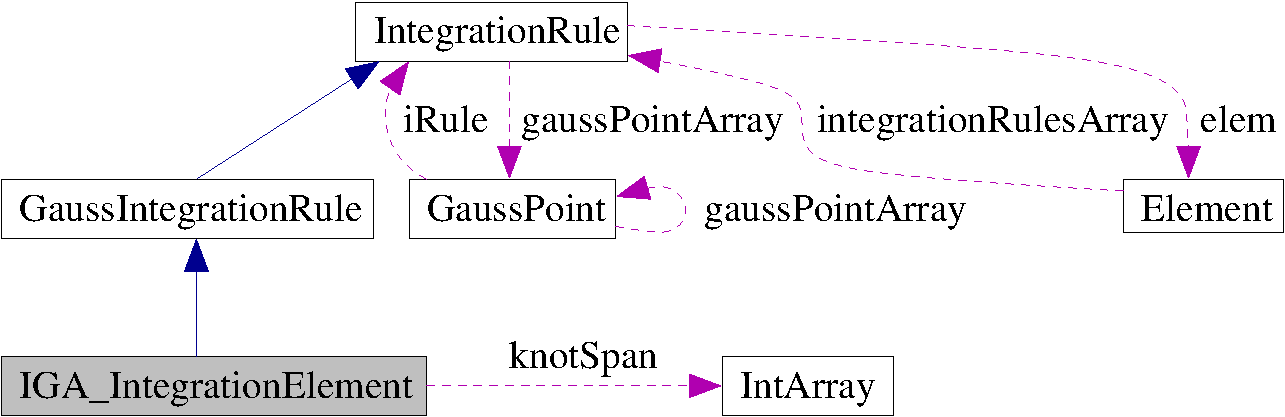
\includegraphics[width=0.7\textwidth]{class_IGA__IntegrationElement_mod.pdf}}
\else
\centerline{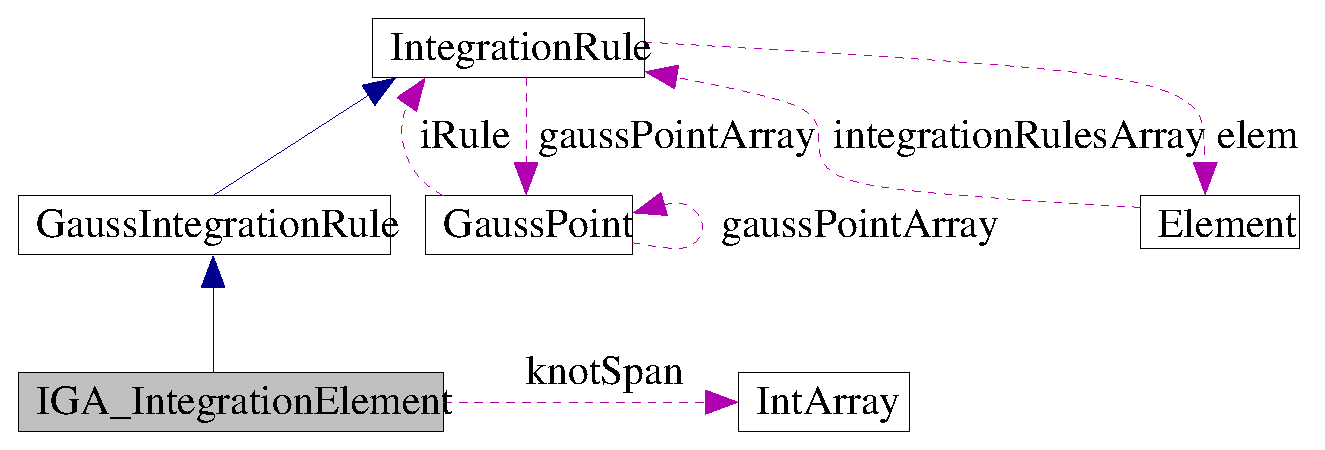
\includegraphics[width=0.7\textwidth]{class_IGA__IntegrationElement_mod.eps}}
\fi
\caption{Collaboration diagram for \class{IGA\_\_IntegrationElement} class.}
\label{IGA__IntegrationElement}
\end{center}
\vspace{-5mm}
\end{figure}

One of the fundamental issues, that has to be addressed at the element
level, is the integration. The integration, usually the Gaussian
integration, is performed over the nonzero knot spans. Individual
integration points are represented 
by \class{GaussPoint} class. They maintain their spatial
coordinates and corresponding integration weights. The individual
integration points are set up and grouped together by base
\class{IntegrationRule} class. For example,
\class{GaussIntegrationRule} class, derived from
\class{IntegrationRule} base, implements Gauss quadrature. An
important feature is that an element may have several integration
rules. This is very useful for the implementation of the reduced or selective
integration, for example. The concept of multiple integration rules
per element is extended in the present context of the IGA. The
\class{IGA\_IntegrationElement} class is introduced to represent the
integration rule for individual nonzero knot spans, see
Figure~\ref{IGA__IntegrationElement}. Since it is derived from
\class{GaussIntegrationRule}, it inherits the capability to set up
Gauss integration points. The reason for creating a~new class is to
introduce the new attribute \attribute{knotSpan}, where the
corresponding  knot span is stored. This information is used in
interpolation class to evaluate corresponding basis functions and
their derivatives at a~given integration point. Note that generally, the
active knot span can be determined for each integration point on the
fly whenever it is needed, but in our approach this information is stored to save
the computational time. The \class{IGA\_IntegrationElement} instances
are set up for each nonzero knot span. The element integration then
consists of a~loop over individual nonzero knot spans, i.e. the loop over
\class{IGA\_IntegrationElement}s and by inner loop over the individual
integration points of the particular knot span.

The individual IGA elements are derived from \class{IGAElement} class,
derived from the base \class{Element}. The purpose of \class{IGAElement}
class is to provide general method for initialization of individual
integration rules on nonzero knot spans (represented by
\class{IGA\_IntegrationElement} class). The integration rules provide
methods to create individual integration points in parametric
space. An efficient implementation requires to map coordinates of
individual integration points with parametric coordinates related to
knot spans directly to knot vector based space. Specific elements are
derived from the base \class{Element} (or  \class{IGAElement} class), that
delivers the generic element part and also from one or more classes
implementing problem-specific functionality, see
Figure~\ref{BSplinePlaneStressElement}. In the presented approach,
\class{StructuralElementEvaluator} is an abstract base class, that
defines the interface for structural analysis, which includes methods
to evaluate mass and stiffness matrices, load vectors, etc. Some of
the methods are already implemented at this level, such as stiffness
matrix evaluation, based on declared abstract services (evaluation of
strain-displacement matrix, etc.), which have to be implemented by
derived classes. The example of the evaluation of the element stiffness matrix,
which can be used by both classical and IGA based elements, is
presented in Table~\ref{stiffness_computation} using symbolic
code.

\begin{figure}[b!]
\begin{center}
\ifpdf
\centerline{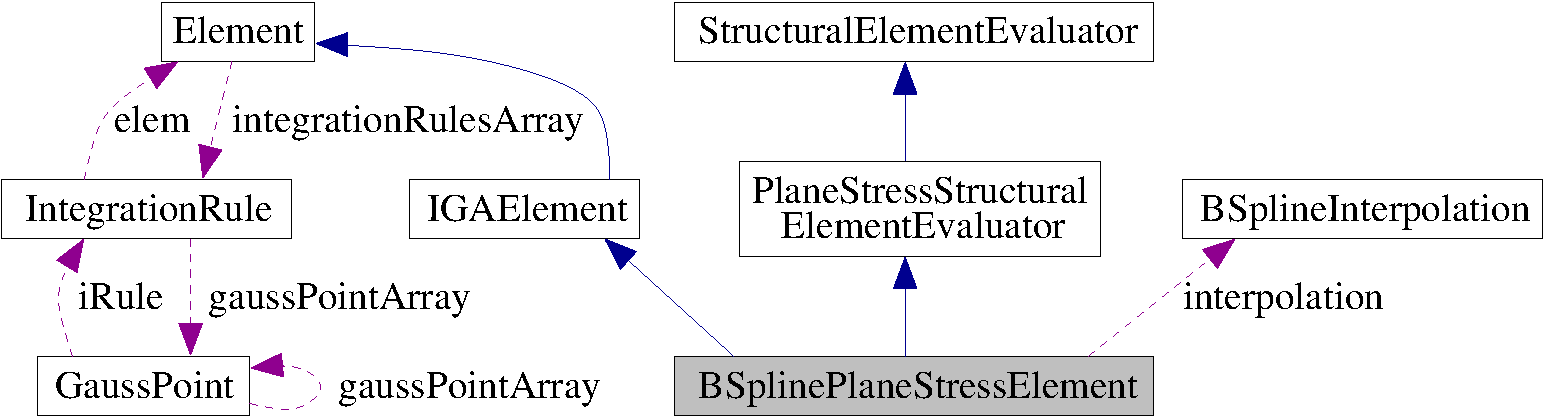
\includegraphics[width=0.7\textwidth]{class_BsplinePlaneStressElement_collaboration.pdf}}
\else
\centerline{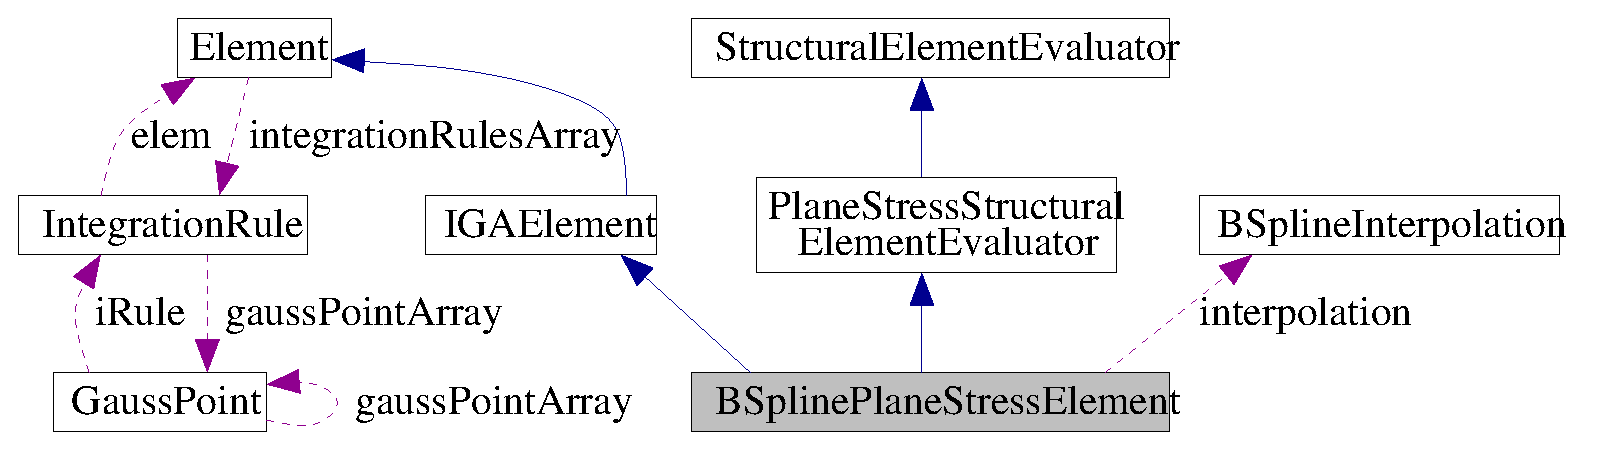
\includegraphics[width=0.7\textwidth]{class_BsplinePlaneStressElement_collaboration.eps}}
\fi
\caption{Collaboration diagram for \class{BSplinePlaneStressElement} class.}
\label{BSplinePlaneStressElement}
\end{center}
\vspace{-5mm}
\end{figure}

\begin{table}[t]
\footnotesize
\begin{verbatim}
StructuralElementEvaluator::computeStiffnessMatrix(){
  loop on all integration rules of the element:
     loop on all Gauss points of the IntegrationRule:
        B = this->computeStrainDisplacementMatrix(gp);
        D = this->computeConstitutiveMatrix(gp);
        dV = this->computeVolumeAround(gp);
        stiffnessMatrix->add(product of B^T_D_B_dV); 
}
\end{verbatim}
\caption{Symbolic code for the evaluation of the stiffness matrix
	(keyword ``this'' means that the called method is provided by the
	class itself).}
\label{stiffness_computation}
\end{table}

In the structural analysis context, classes derived from
\class{StructuralElementEvaluator} implement desired functionality for
specific types of structural analyzes (plane-stress, plane-strain,
full 3D, etc). Provided that the element defines its interpolation
(B-spline basis functions), it is
possible to evaluate remaining abstract methods from
\class{StructuralElementEvaluator} interface. This is illustrated in
Table~\ref{strain_displacement_computation} on an example of the
evaluation of the strain-displacement matrix for the case of plane
stress analysis. Thus, when a~new element is 
defined, it has to create its own interpolation and should be derived from
\class{Element} class, which delivers the general basic element
functionality and from one or more evaluators, implementing
analysis-specific functionality. Such a~design, based on 
decoupled representation of element interpolation and problem specific
evaluators, has several advantages. It allows to define problem
specific methods only once for several elements with different geometry and
interpolation and allows straightforward implementation of elements
for multi-physics simulations. 

\begin{table}[t]
\footnotesize
\begin{verbatim}
PlaneStressStructuralElementEvaluator::
computeStrainDisplacementMatrix(IntegrationPoint gp) {
   FEInterpolation interp = gp->giveElement()->giveInterpolation();
   interp->evalShapeFunctDerivatives (der, gp);
 
   answer.resize(3, nnode*2);              // 2 DOFs per each node
   answer.zero();
  
   for i=1:nnode
     // epsilon_x
     answer.at(1, i*2-1) = der.at(i, 1);   // dN(i)/dx
     // epsilon_y
     answer.at(2, i*2)   = der.at(i, 2);   // dN(i)/dy
     // shear strain
     answer.at(3, i*2-1) = der.at(i, 2);   // dN(i)/dy
     answer.at(3, i*2)   = der.at(i, 1);   // dN(i)/dx
}
\end{verbatim}
\caption{Symbolic code for the evaluation of the strain-displacement matrix.}
\label{strain_displacement_computation}
\end{table}

The description of the element interpolation is encapsulated into a~class
derived from \class{FEInterpolation} class which defines the
abstract interface in terms of services that evaluate shape
functions, their derivatives, jacobian matrix, etc. at given
point. In the frame of presented work, the
%\class{BSplineInterpolation} or \class{NurbsInterpolation} classes
%have been implemented. 
\class{BSplineInterpolation} class has been implemented.
Each finite element has to set up its
interpolation and provide access to it. This is enforced by general
\class{Element} interface, that requires to define the method for
accessing element interpolation. The abstract \class{FEInterpolation}
class interface is essential, as it allows to implement problem
specific element methods already at the top level (like the evaluation of
element interpolation or strain-displacement matrices). An efficient
implementation should profit from the locality of
individual interpolation functions which have limited support over
several consecutive knot spans. Therefore methods
declared by \class{FEInterpolation} class evaluating values of
interpolation functions or their derivatives return the values
only for those, that are nonzero in actual knot span. This
enables to compute characteristic element contributions on a~knot span
basis efficiently. For each individual knot span, the contributions are
computed only for generally nonzero shape functions and then are
localized into element contribution. The mask of nonzero shape
functions for individual knot spans can be evaluated using
\service{giveKnotBasisFuncMask} service declared by
\class{FEInterpolation} and really provided by \class{BSplineInterpolation}.




\section{Miscellaneous}
\subsection{Vectors and Matrices}
The OOFEMlib provides the abstraction for integer vectors (\class{IntArray})
and for real vectors and matrices (\class{FloatArray} and
\class{FloatMatrix}). The usual arithmetic operations (like vector and
matrix additions, substractions, matrix vector multiplication, matrix
inverse, solution of linear system, finding eigenvalues and
eigenvectors) are provided. Hovewer, the usual math operators ('+','*')
are not overloaded, user has to call specific routines. 
The vector and matrices provide both 0-based and 1-based component
access, they allow for dynamicall resize with optinal chunk. In fact,
the current implementation of \service{resize} only grows the
receiver, the possible request for shring does not cause the
realocation of memory, since allocated memory is kept for future possible resize. If
resize operation wants to force allocation, then \service{hardResize}
should be invoked instead. 
The prefered argument passing is by reference, even for function or
procedure return values.
The called function performs resize and fills up
the return parametr(s). This is motivated by aim to avoid memory
allocation/dealocation problems. The programer should always avoid to
return pointers to newly allocated arrays or matrices. 
See section ``Coding Standards'' for
details.

\subsection{Solution Step} 
Class representing solution step. The Solution step instance may represent either 
time step, load increment, or load case depending on current Engineering model used.

Solution step maintain the reference to correspoding Engineering model class instance.
It maintain also its "intrinsic time" and corresponding time increment. The meaning of these 
values is dependent on current Engineering model used. The time may represent either
current time, load increment number or load case number. See corresponding 
Engng model reference for details.
	
Some components (typically integration points real stresses or integration points nonlocal values)
are computationally wery demanding. Because in typical code, there are number of requests for same value 
during the computation process, it may be efficient to store these values and compute them only once.
The principal problem is to recognize, when is necessary to re-compute these stored values to reflect 
newly reached state. This cannot be determined form solution step "time", because solution step may 
represent for example load increment, inside which typically many iterations are needed to reach 
convergence. For this purpose, a concept of solution state counters is provided.
Whenever the solution state changes, the engineering model updates the solution state counter.
The solution state counter is guaranteed to grow up smoothly (it newer decreases) during solution process.
Other components of program (integration points) can then store their computationally expensive values
but have to store also corresponding solution state counter value valid when these were computed.
Then their can easily check for difference between freezed solution state counter for their value with 
current solution state requested from solution step and recompute the values if necessary.

\subsection{Load Time Functions}
Abstract base class representing load time function. Classes derived from Load class typically 
describe load from spatial point of view. The purpose of introducing load time function is to express
variation of some components in time. Load time function typically belongs to domain and is 
attribute of one or more loads. Generally load time function is real function of time ($y=f(t)$).

\section{Coding Standards}
\subsection{Naming Conventions}

The names of classes, attributes, services, variables, and functions
in a program serve as comments of a sort. So don't choose terse names--instead, look for names that give useful information about the meaning of the variable or function. In a OOFEM
program, names should be English, like other comments. 

Local variable names can be shorter, because they are used only within one context, where (presumably) comments explain
their purpose. 

Try to limit your use of abbreviations in symbol names. It is ok to make a few abbreviations, explain what they mean, and
then use them frequently, but don't use lots of obscure abbreviations. 

Please use capital letters to separate words in a name. Stick to
lower case; reserve upper case for macros, and for name-prefixes that
follow a uniform convention. The function or service name should always begin with lovercase
letter, the first uppercase letter in function name indicates, that
function is returning newly allocated pointer, which has to be dealocated.
For example, you should use names like ignoreSpaceChangeFlag; 

When you want to define names with constant integer values, use enum rather than `\#define'. GDB knows about
enumeration constants. 

Use descriptive file names. The class declarations should be placed in *.h files
and class implementation in corresponding *.C files. For each class, create a separate files.


\subsection{Parameters and Return Values}

The prefered argunent passing method for objects is by reference. 
Try to avoid rerturning pointers to arrays or matrices (or generally
to any component), since it is not clear, whether to delocate the
returned pointer or not. The most prefered way is to create local
variable of vector or matrix type, pass it (using reference) to called
function. The calling function is responsible to properly resize the
(output) parameter and set values accordingly. The point is, that
destructors are called for local variables automatically by compiler,
so there is no possibility for memory leaks and the local variable can
be reused for multiple calls to target function (inside loop) and
therefore there is no need for repeating memory allocation and
dealocation. Sometimes it may be reasonable to return pointer to
constant float array or matrix (representing for example
nodal coordinates), since passing output array as parametr will require 
array copying. 

\subsection{Interface concept}
Interfaces provide a way, how to organize or group optional or function-specific services into 
clearly defined units (well structured code) which can be
selectivelly implemented by some classes.

The interface concept can be ilustrated on following simple example. 
Let's have an error estimator, represented by corresponding class. This estimator requires some special 
services at the element level. Because typically not all elements provide support for this error estimator,
it would be wasting of space to declare required services in general element base class.
(This will lead to big and extremly general interface declared by base class, 
with only some services compulsory and with many optional services. This can lead to confusion and very unclear structure).
Suggested remedy is to declare corresponding interface to error estimator. The interface 
should declare all servics needed by error estimator. Particular elements, which would like to provide support for
error estimator, simply derive itself from corresponding interface and implement services from interface.
If error estimator wants to access its interface, it asks element for pointer to its corresponding interface
(getInterface method). Once interface is returned, error estimator can use its services to compute response.

Some dificulty may arise, when implementing general interface service, reguiring general services
from class implementing interface. Then simple "trick" can be made:
The interface should declare service giveClass(), which returns the pointer to class which implements interface.
After having this pointer, the interface general service can use all (but only public) services of class implementing
interface. For example some service utilizing the integration over element volume can be formulated as general,
but when interface is defined, there is no connection to element implementing it. This connection can be established
by declaring virtual giveElement() service, which returns the pointer to element implementing the interface. 
Then general implementation at interface class level can be made, using base Elment class public services. 
Then all element classes implementing the interface should overload only giveElement service, but not the whole 
service with integration.

To facilitate the interface concept, the abstract class
\class{Interface} is introduced. Its role is to provide a base class for all interfaces. 
The interface represent some well defined additional or optional ability or support, which is provided by some class.
The services and attributes required are encapsulated in particular
derived interface class, which is derived from base \class{Inferface} class.
The class which wants to implement interface will simply inherits corresponding interface class.
Each base class, whose derived classes are assumed to implement some interfaces, will declare
the virtual getInterface(InterfaceType) method. This method must be implemented by each derived class implementing
some interface and returns pointer to corresponding interface. This
service then provides general way, how to
access particular interface of given class. 
	
\clearpage

%\fig[t]{0mm\label{microplaneFig}\centerline{\epsfbox{microplaneSm.eps}}}           %obr.1
%{General Structure}

%\vskip20mm
%\vskip20mm

\addcontentsline{toc}{section}{Acknowledgments}
\section*{Acknowledgments}
This work was supported by the Grant Agency of the Czech Republic -
Project No.: 103/97/P106.

%\vfill
\addcontentsline{toc}{section}{References}
\begin{thebibliography}{9}

\bibitem{CoadYourdon}COAD, P. and YOURDON, E.: {Object-Oriented Analysis,} Prentice-Hall,  1991.

\bibitem{DP}DUBOIS-PELERIN, Y.: {Object-Oriented  Finite Elements:
Programming concepts and Implementation,} PhD Thesis, EPFL, Lausanne, 1992.

\bibitem{ke-ri} KERNINGHAM, B.W. and RITCHIE, D.M.: {The C Programming
Language,} Prentice-Hall, 1978.

\bibitem{oofem} PATZ\'{A}K, B.: {OOFEM Project home page,}
http://ksm.fsv.cvut.cz/oofem/oofem.html, 2000.

\bibitem{pat} PATZ\'{A}K, B.: {V\'{y}po\v{c}etn\'{\i} modely pro beton,} PhD
thesis, in Czech, FSv \v{C}VUT 1996. 

\bibitem{pat2} PATZ\'{A}K, B. and RYPL, D. and BITTNAR, Z.: {Object
oriented finite element modelling,} In B.H.V. Topping and B. Kumar, editors,
Developments in Analysis and Design using Finite Elements
Methods. Civil-Comp Press, 1999. ISBN 0 9487 4961 X. 

\bibitem{pat3} PATZ\'{A}K, B.:{Object oriented finite element modeling,} ACTA POLYTECHNICA, 39(2/1999):99-113, 1999. ISSN
1210-2709. 

\bibitem{pat4} PATZ\'{A}K, B. and BITTNAR, Z.:{Design of object
oriented finite element code}, Advances in Engineering Software,
32(10-11):759--767, 2001. 

\bibitem{RypPat} Rypl, D., Patz\'{a}k, B.: {bject Oriented Framework for the Isogeometric Analysis}, In Topping, B.H.V., Costa Neves L.F., Barros R.C., editors, CD-ROM Proceedings of the Twelfth International Conference on Civil, Structural and Environmental Engineering Computing, Civil-Comp Press, 2009. ISBN 978-1-905088-31-7.

\bibitem{ChaPat} R. Chamrov\'{a} and B. Patz\'{a}k. On xfem integration within an object-oriented finite element code. In B. H. V. Topping, L. F. Costa Neves, and R. C. Barros, editors, Proceedings of the Twelfth International Conference on Civil, Structural and Environmental Engineering Computing, Stirlingshire, United Kingdom, 2009. Civil-Comp Press. paper 276.

\bibitem{c++} STROUSTRUP, B.: {The C++ Programming Language - 3rd ed,}
Addison-Wesley, 1997.

\bibitem{zimm} ZIMMERMANN, T., DUBOIS-PELERIN, Y., and BOMME, P.: {Object-oriented finite element programming: I. Governing principles,} Comp. Meth. in Appl. Mech. Engng., 98(3), 291-303, 1992. 
\end{thebibliography}

\end{document}


